\documentclass[a4paper, 11pt]{article}

%%% Работа с русским языком
\usepackage{cmap}					% поиск в PDF
\usepackage{mathtext} 				% русские буквы в формулах
\usepackage[T2A]{fontenc}			% кодировка		% кодировка исходного текста
\usepackage[english,russian]{babel}	% локализация и переносы

%%% Дополнительная работа с математикой
\usepackage{amsfonts,amssymb,amsthm,mathtools} % AMS
\usepackage{amsmath}
\usepackage{icomma} % "Умная" запятая: $0,2$ --- число, $0, 2$ --- перечисление

\usepackage{indentfirst} % Красная строка в начале абзацев

\usepackage{setspace} % Междустрочный интервал
\singlespacing

\usepackage[left=20mm, top=10mm, right=10mm, bottom=25mm, nohead, footskip=7mm]{geometry} % поля документа

%% Номера формул
%\mathtoolsset{showonlyrefs=true} % Показывать номера только у тех формул, на которые есть \eqref{} в тексте.

%% Шрифты
\usepackage{euscript}	 % Шрифт Евклид
\usepackage{mathrsfs} % Красивый матшрифт

%% Перенос знаков в формулах (по Львовскому)
\newcommand*{\hm}[1]{#1\nobreak\discretionary{}
    {\hbox{$\mathsurround=0pt #1$}}{}}

%%% Работа с картинками
\usepackage{graphicx}  % Для вставки рисунков
\graphicspath{{images/}{images2/}}  % папки с картинками
\setlength\fboxsep{3pt} % Отступ рамки \fbox{} от рисунка
\setlength\fboxrule{1pt} % Толщина линий рамки \fbox{}
\usepackage{wrapfig} % Обтекание рисунков и таблиц текстом

%%% Работа с таблицами
\usepackage{array,tabularx,tabulary,booktabs} % Дополнительная работа с таблицами
\usepackage{longtable}  % Длинные таблицы
\usepackage{multirow} % Слияние строк в таблице


\usepackage[utf8]{inputenc}
\usepackage[russian]{babel}
\usepackage{amsmath,amsfonts,amssymb,amsthm,mathtools} %AMS

\usepackage{hyperref}  % Гиперссылки
\usepackage[usernames,dvipsnames,svgnames,table,rgb]{xcolor}
\usepackage{enumitem} %Для нумерации списков
\usepackage{multicol} % Несколько колонок
\usepackage{multirow} % Несколько строк
%\usepackage{caption} % отступы между названием и объектом
%\captionsetup[images]{skip=2ex}

\usepackage{dsfont}

\DeclareMathOperator*{\argmax}{arg\,max}

\hypersetup{
    unicode=true,
    pdftitle={Практическое задание №2}, % Заголовок
    pdfauthor={Кузьмин Никита, ММП 317},
    pdfcreator={Кузьмин Никита, ММП 317},
    colorlinks=false, % false - ссылки в рамках; true - цветные ссылки
    linkcolor=red,   % внутренние ссылки
    citecolor=green, % на библиографию
    filecolor=magenta, % на файлы
    urlcolor=blue % на URL
}



%\usepackage{titlesec}

%\titleformat*{\section}{\LARGE\bfseries}
%\titleformat*{\subsection}{\Large\bfseries}
%\titleformat*{\subsubsection}{\large\bfseries}

\usepackage{sectsty}
\sectionfont{\LARGE}
\subsectionfont{\LARGE}
\subsubsectionfont{\Large}
\usepackage{float}


\usepackage{fancyhdr}% загрузим пакет
%\pagestyle{fancy}% применим колонтитул

\begin{document}
    \hfill Кузьмин Никита, ММП, 317.
    
    \begin{center} \Large Отчет по практическому заданию №2 "\textbf{Применение линейных моделей для определения токсичности комментария}". 
    
    Логистическая регрессия и градиентный спуск.
    \tableofcontents
    \end{center}
    
    \newpage
    \section{Введение}
    
    В данном документе представлен отчет о проделанных экспериментах по практическому заданию №2, анализ результатов. 
    Краткое описание задания: необходимо реализовать линейный классификатор с произвольной функцией потерь.
    
    \section{Эксперименты}
    В этом блоке приведены все обязательные эксперименты, которые изложены в формулировке задания.
    Все эксперименты проводились на упрощенном датасете (рассматривается задача бинарной классификации) из соревнования \textbf{Toxic Comment Classification Challenge}, в котором нужно определить токсичность комментария. 
    
    Стандартный дизайн эксперимента: 
    \begin{itemize}
        \item Оценка качества и подбор параметров модели проводились на каждой эпохе с помощью отложенной тренировочной выборки (30\%). Все графики ниже построены по значениям accuracy, посчитанным на отложенной выборке.
        \item В тренировочную выборку был добавлен признак, состоящий из всех единиц, который позволяет учитывать смещение (\textbf{bias}). Было решено не использовать смещение в $L2$-регуляризации, чтобы даже при плохом выборе коэффициента регуляризации решающая гиперплоскость не вырождалась в 0.
        \item В стохастическом градиентном спуске проверяется критерий останова на каждой эпохе (не итерации).
    \end{itemize}

        \subsection{Исследование поведения градиентного спуска}
            Обновления весов модели при использовании градиетного спуска происходит по следующей формуле:
            \begin{equation}\label{exp1:weight_upd}
            w_t = w_{t-1} - \frac{\alpha}{t^\beta} \times \frac{1}{N} \times \sum_{i=1}^{N}\nabla_{w}\mathcal{L}(x_i, y_i|w_{t-1}),
            \end{equation}
            где $t$ - номер итерации, $\beta$ - \textbf{step\_beta}, $\nabla_{w}\mathcal{L}(x_i, y_i|w_{t-1})$ - градиент функции потерь.
            \subsubsection{Параметр размера шага \textbf{step\_alpha}}
                Параметр \textbf{step\_alpha $(\alpha)$} используется в градиентном спуске при обновлении весов в формуле \ref{exp1:weight_upd}.
                Рассмотрим следующие зависимости при разных значениях параметра \textbf{step\_alpha}:
                    \begin{enumerate}\label{exp:dependencies}
                        \item зависимость значения функции потерь от реального времени работы метода
                        \item зависимость точности (accuracy) от реального времени работы метода
                        \item зависимость значения функции потерь от итерации метода
                        \item зависимость точности (accuracy) от итерации метода
                     \end{enumerate}
                 Соответствующие графики приведены на: рис. \ref{exp1:gd_func_time}, \ref{exp1:gd_acc_time}, \ref{exp1:gd_func_iter}, \ref{exp1:gd_acc_iter}.
   
                 \begin{figure}[H] \label{exp1}
                     \begin{multicols}{2}
                         \begin{center}
                             \caption{Зависимость значения функции потерь от реального времени работы градиентного спуска} \label{exp1:gd_func_time}
                             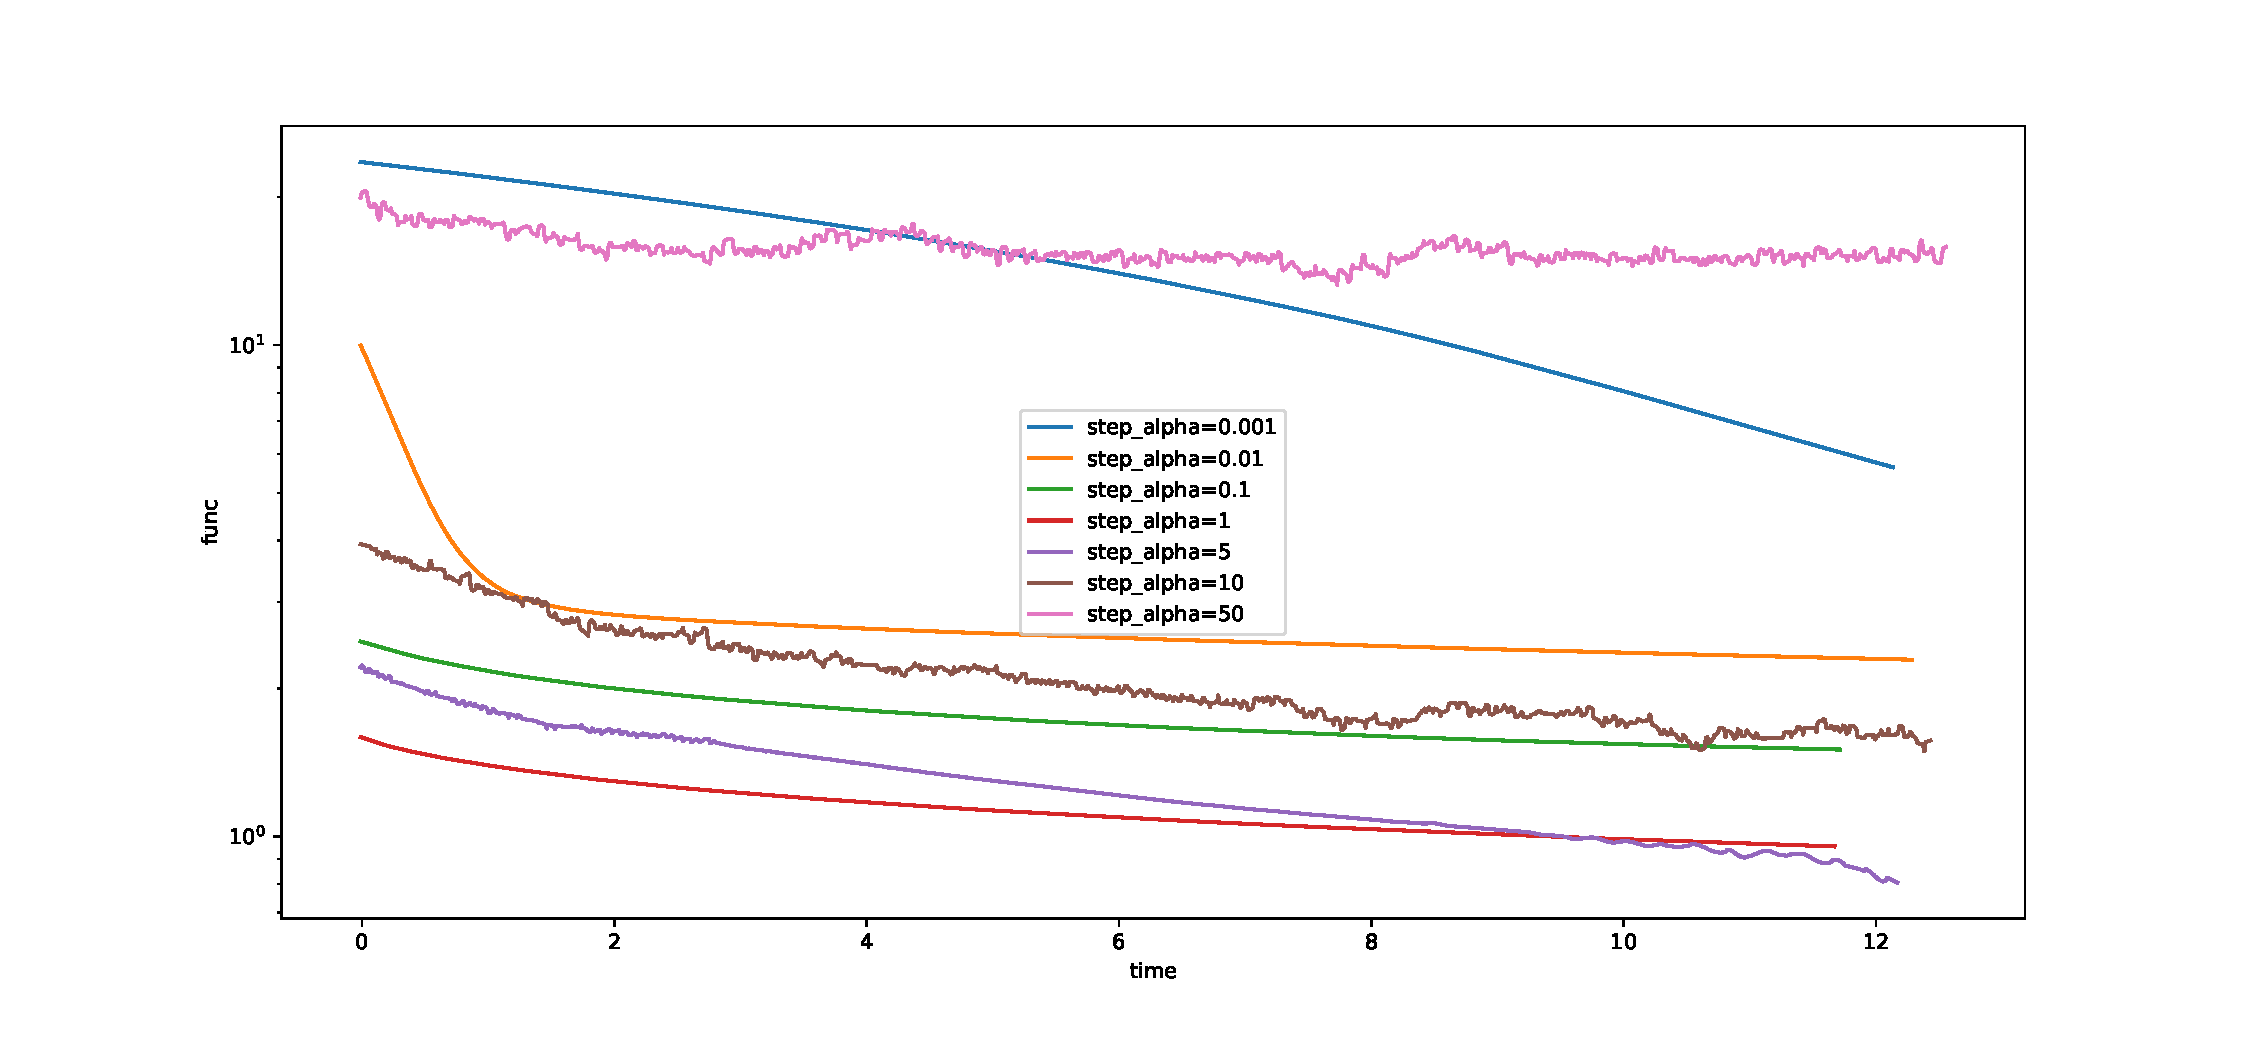
\includegraphics[width=0.5\textwidth, height=0.25\textheight]{../graphs/exp1_func_GD_alpha_time_beta=0,001.pdf}
                             
                             \caption{Зависимость значения точности (accuracy) от реального времени работы градиентного спуска} \label{exp1:gd_acc_time}
                             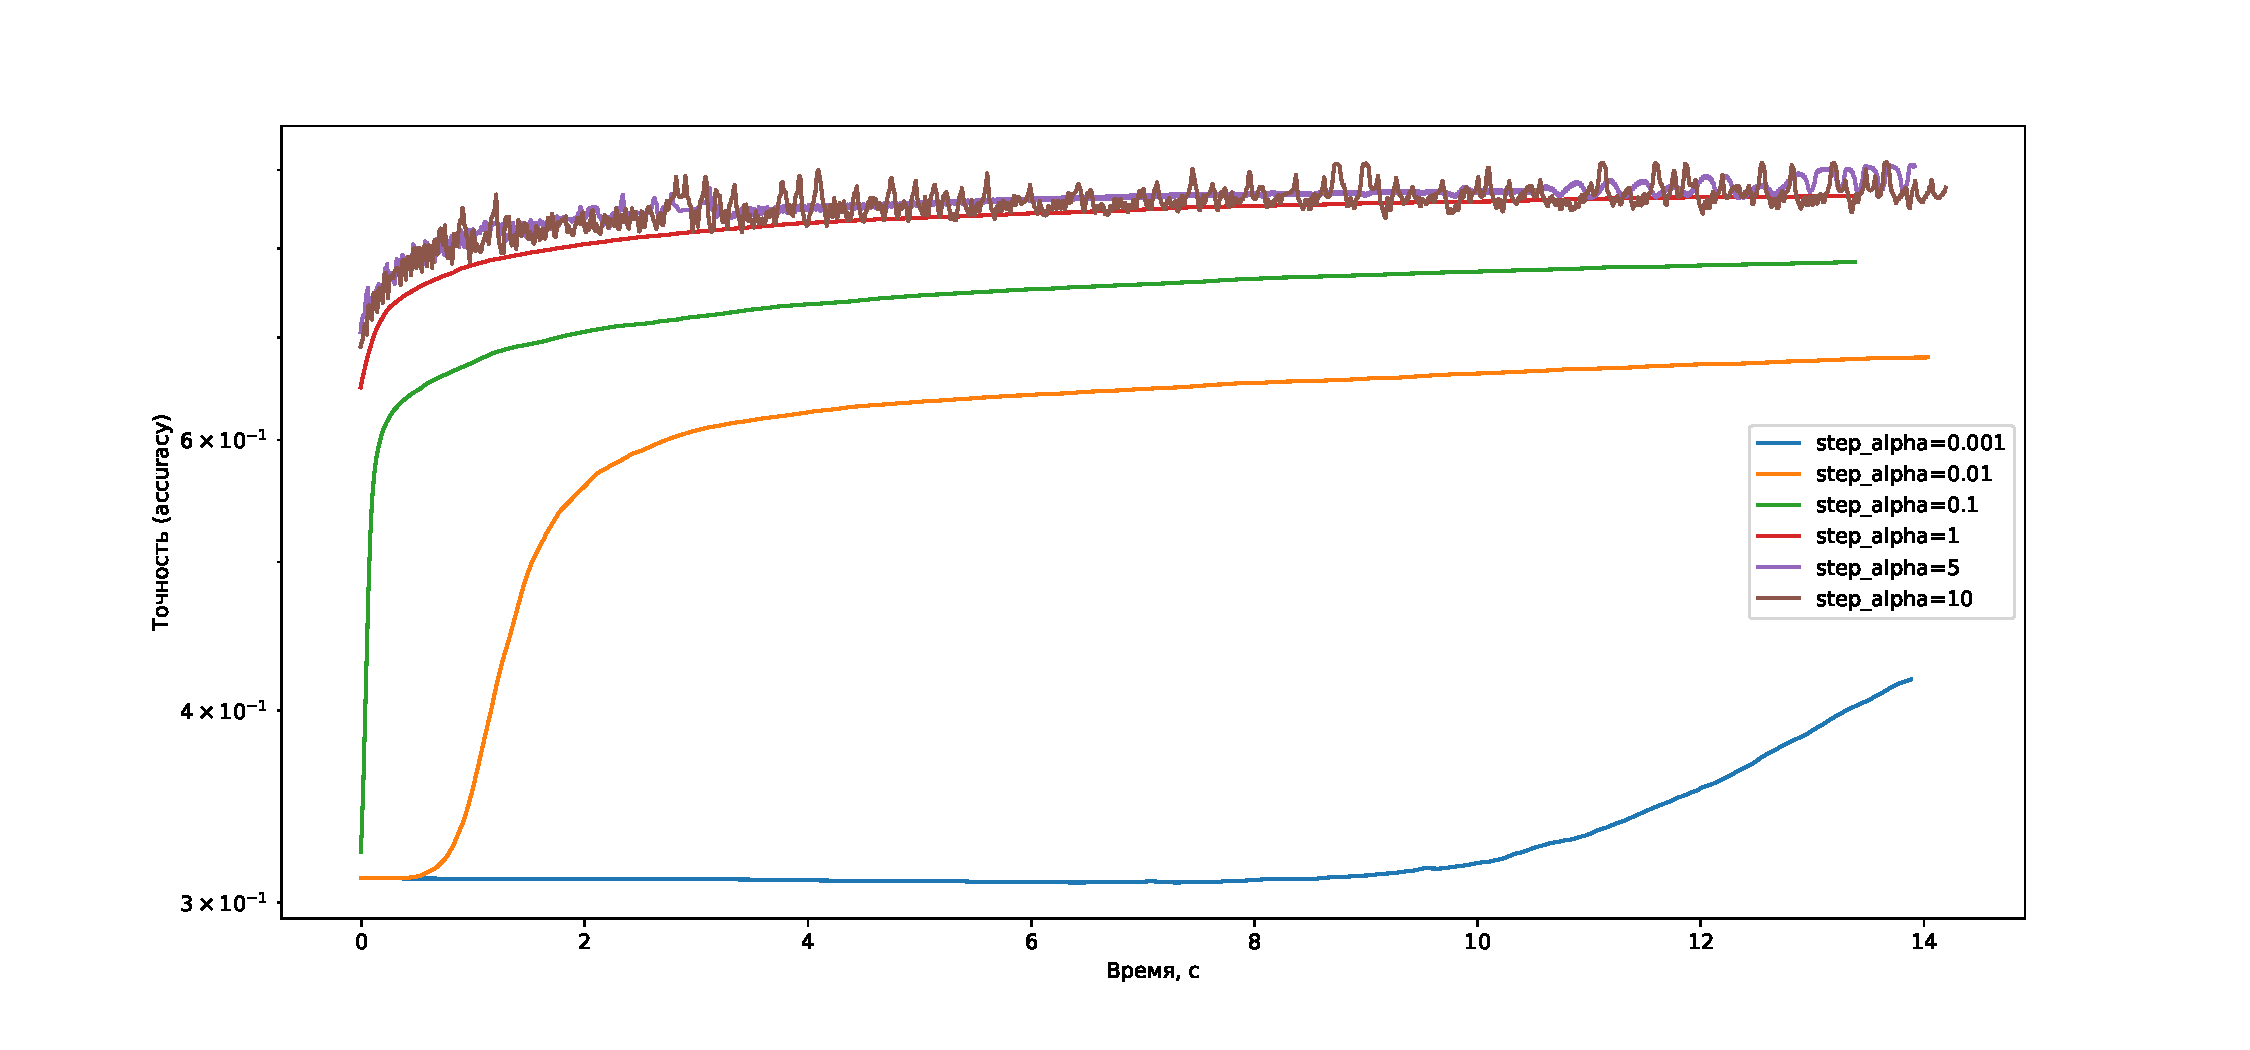
\includegraphics[width=0.5\textwidth, height=0.25\textheight]{../graphs/exp1_accuracy_GD_alpha_time_beta=0,001.pdf}
                             
                             \caption{Зависимость значения функции потерь от итерации метода градиентного спуска} \label{exp1:gd_func_iter}
                             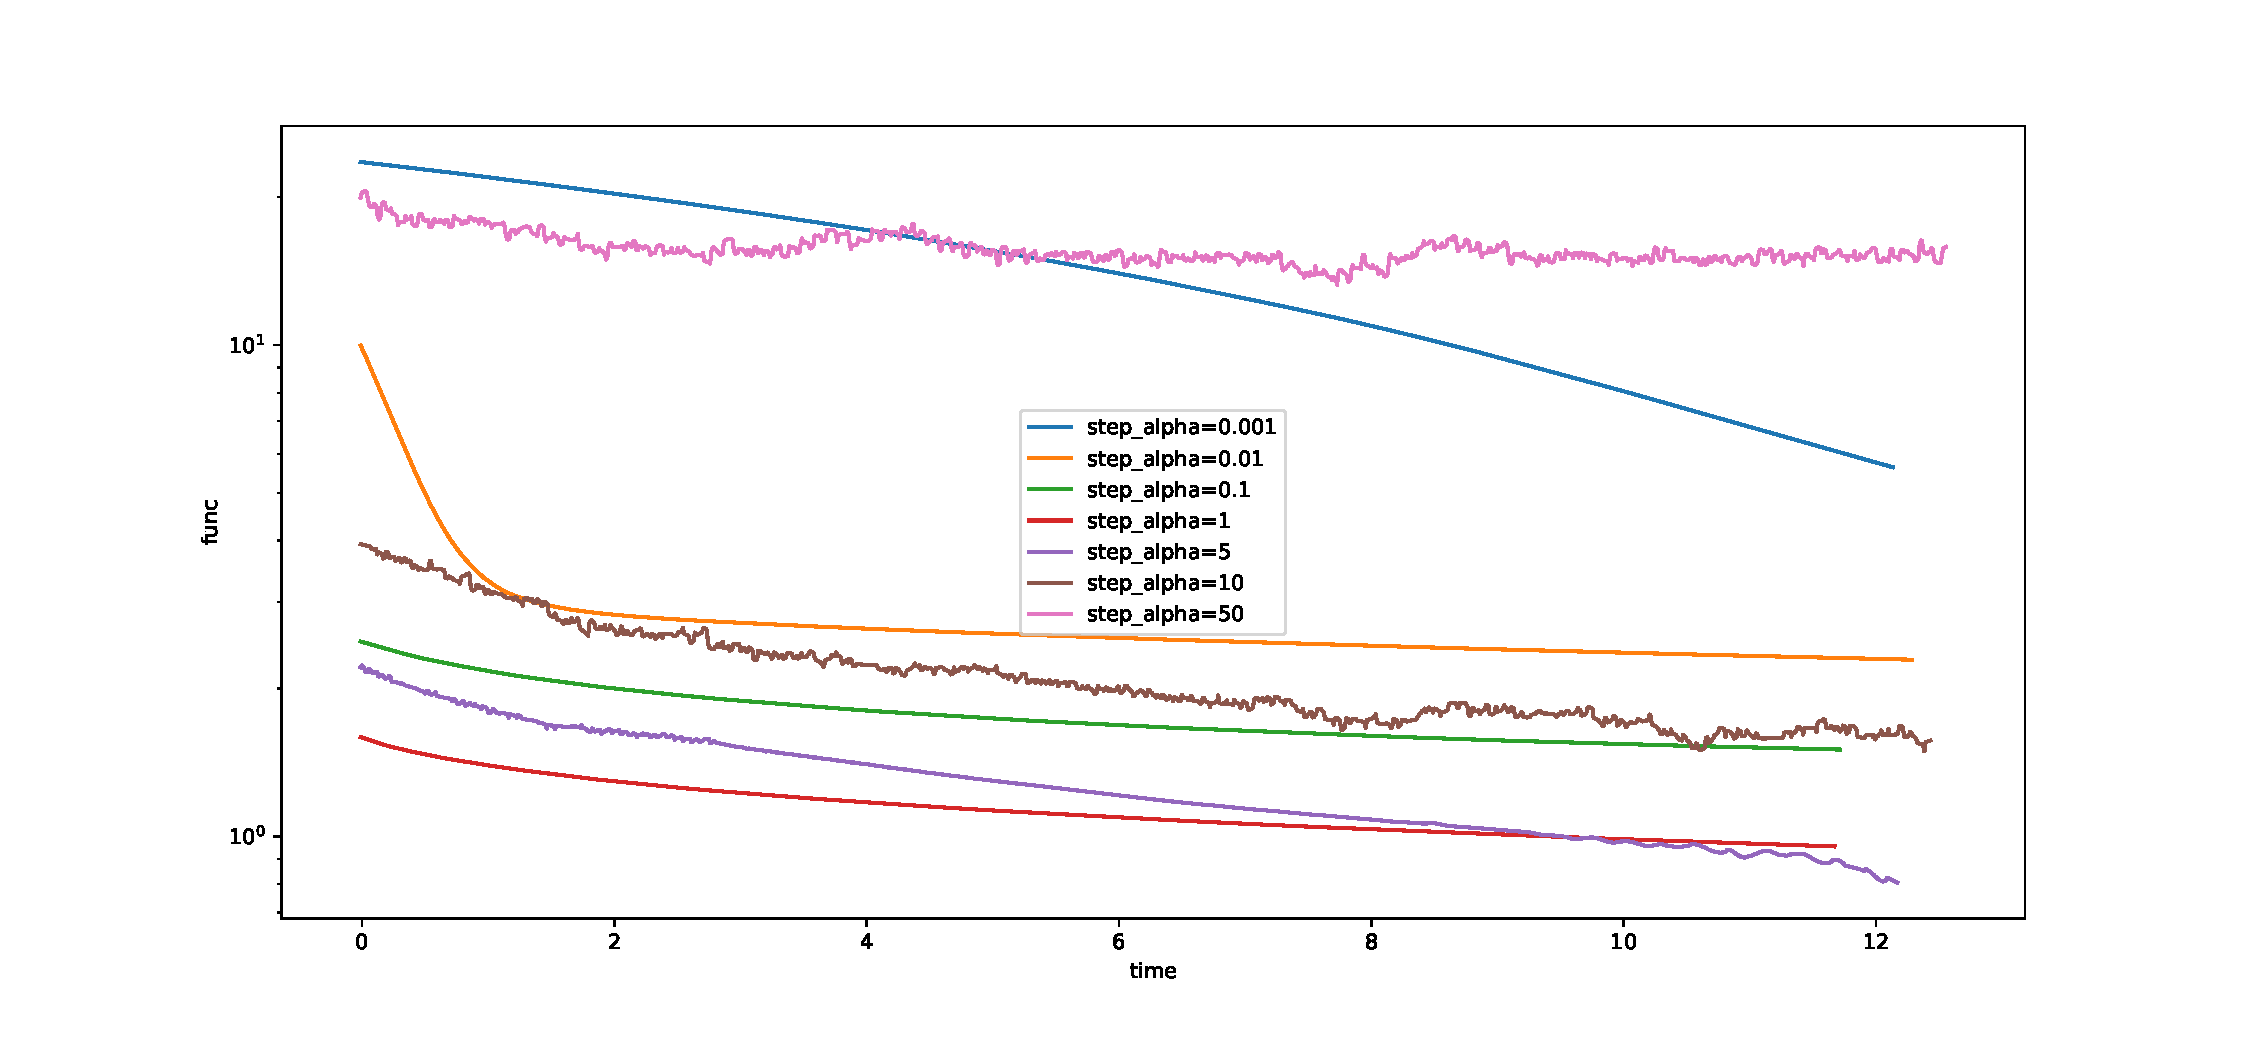
\includegraphics[width=0.5\textwidth, height=0.25\textheight]{../graphs/exp1_func_GD_alpha_time_beta=0,001.pdf}
                             
                             \caption{Зависимость значения точности (accuracy) от итерации метода градиентного спуска} \label{exp1:gd_acc_iter}
                             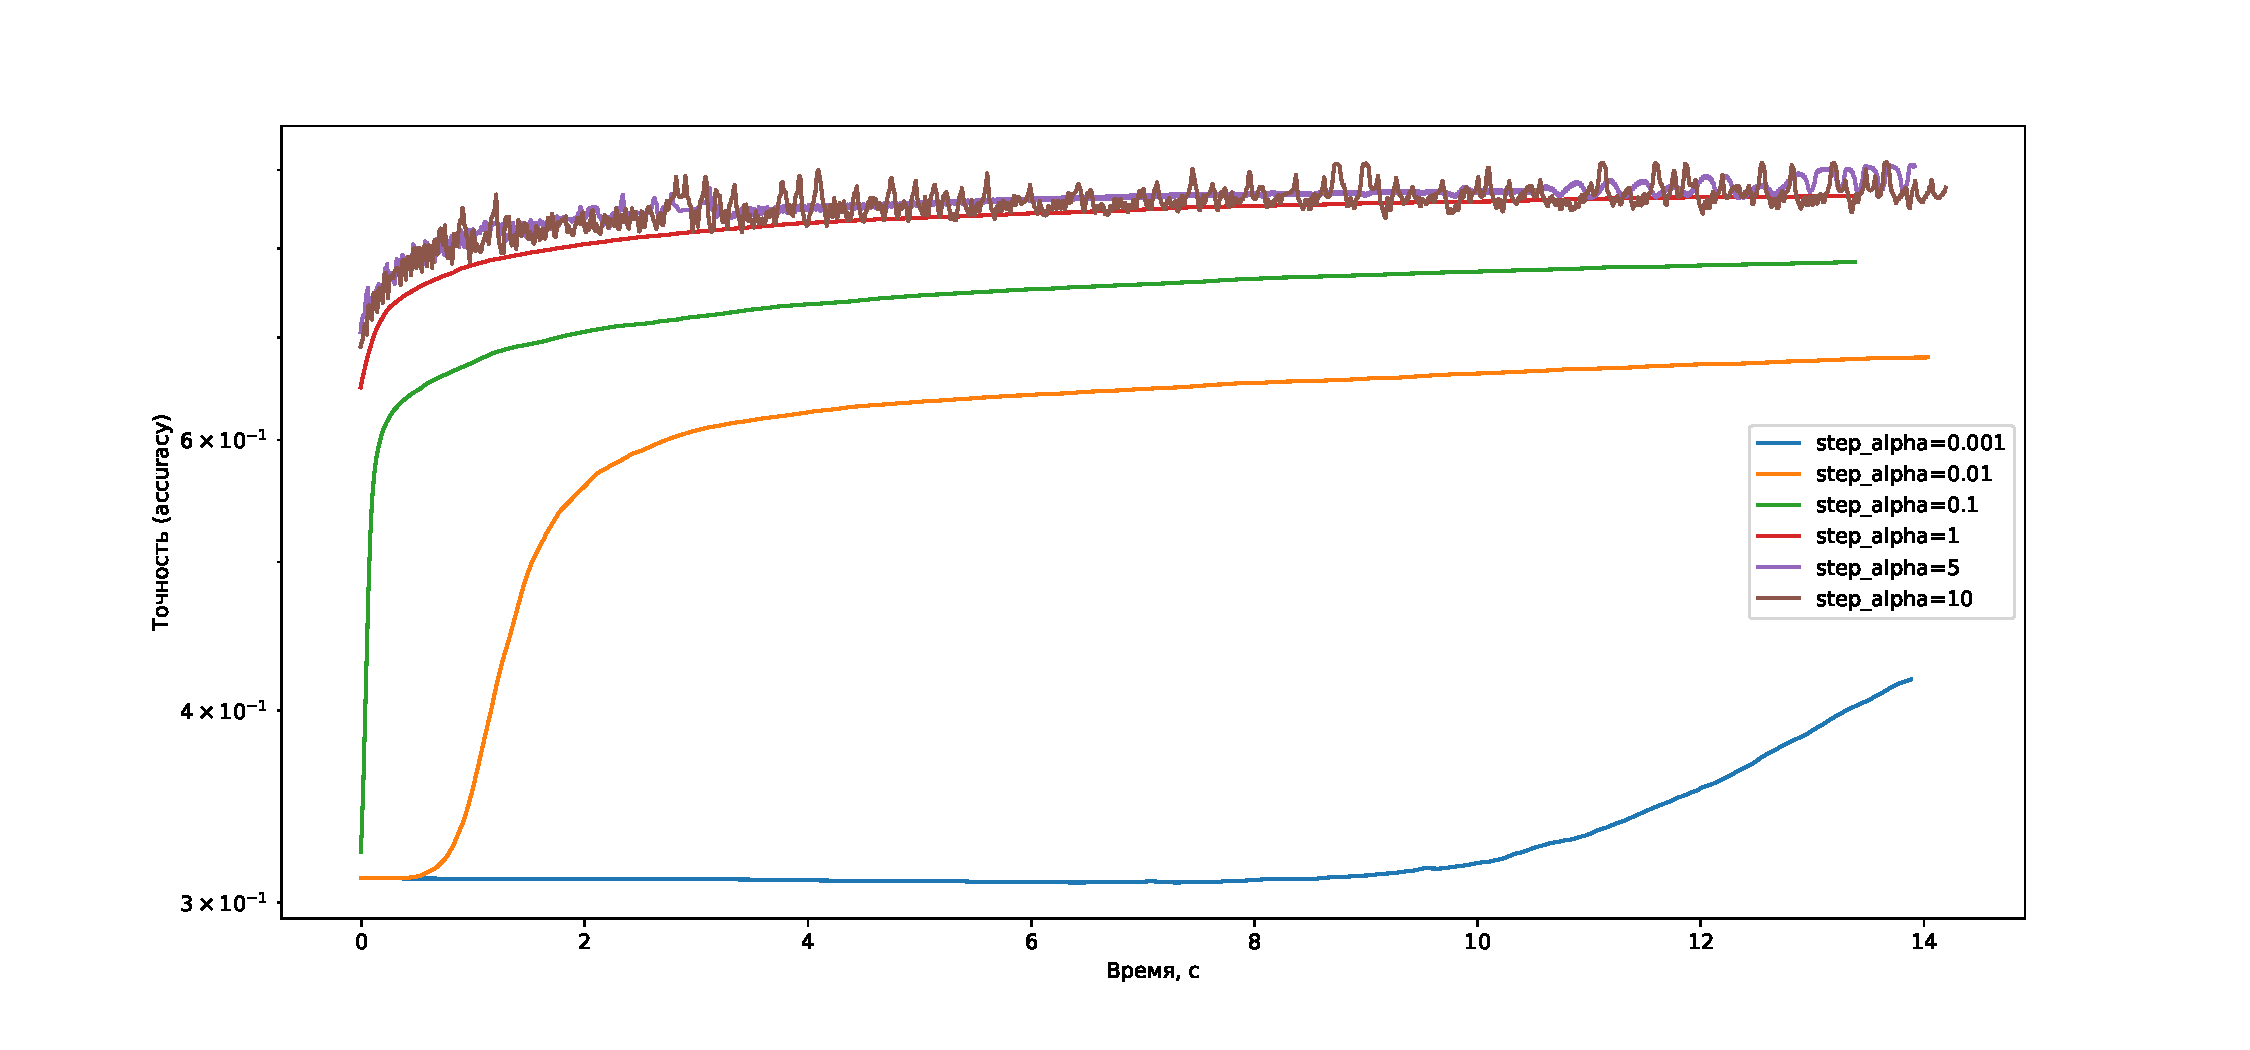
\includegraphics[width=0.5\textwidth, height=0.25\textheight]{../graphs/exp1_accuracy_GD_alpha_time_beta=0,001.pdf}
                         \end{center}
                     \end{multicols}
                 \end{figure}
            \subsubsection{Параметр размера шага step\_beta}
                Параметр \textbf{step\_beta $(\beta)$} используется в градиентном спуске при обновлении весов в формуле \ref{exp1:weight_upd}.
                Аналогично предыдущему пункту рассмотрим зависимости из \ref{exp:dependencies} при разных значениях параметра \textbf{step\_beta} и проанализруем соответсвующие графики, представленные на рис. \ref{exp2:gd_func_time}, \ref{exp2:gd_acc_time}, \ref{exp2:gd_func_iter}, \ref{exp2:gd_acc_iter}.
                
                
                \begin{figure}[H] \label{exp1}
                    \begin{multicols}{2}
                        \begin{center}
                            \caption{Зависимость значения функции потерь от реального времени работы градиентного спуска} \label{exp2:gd_func_time}
                            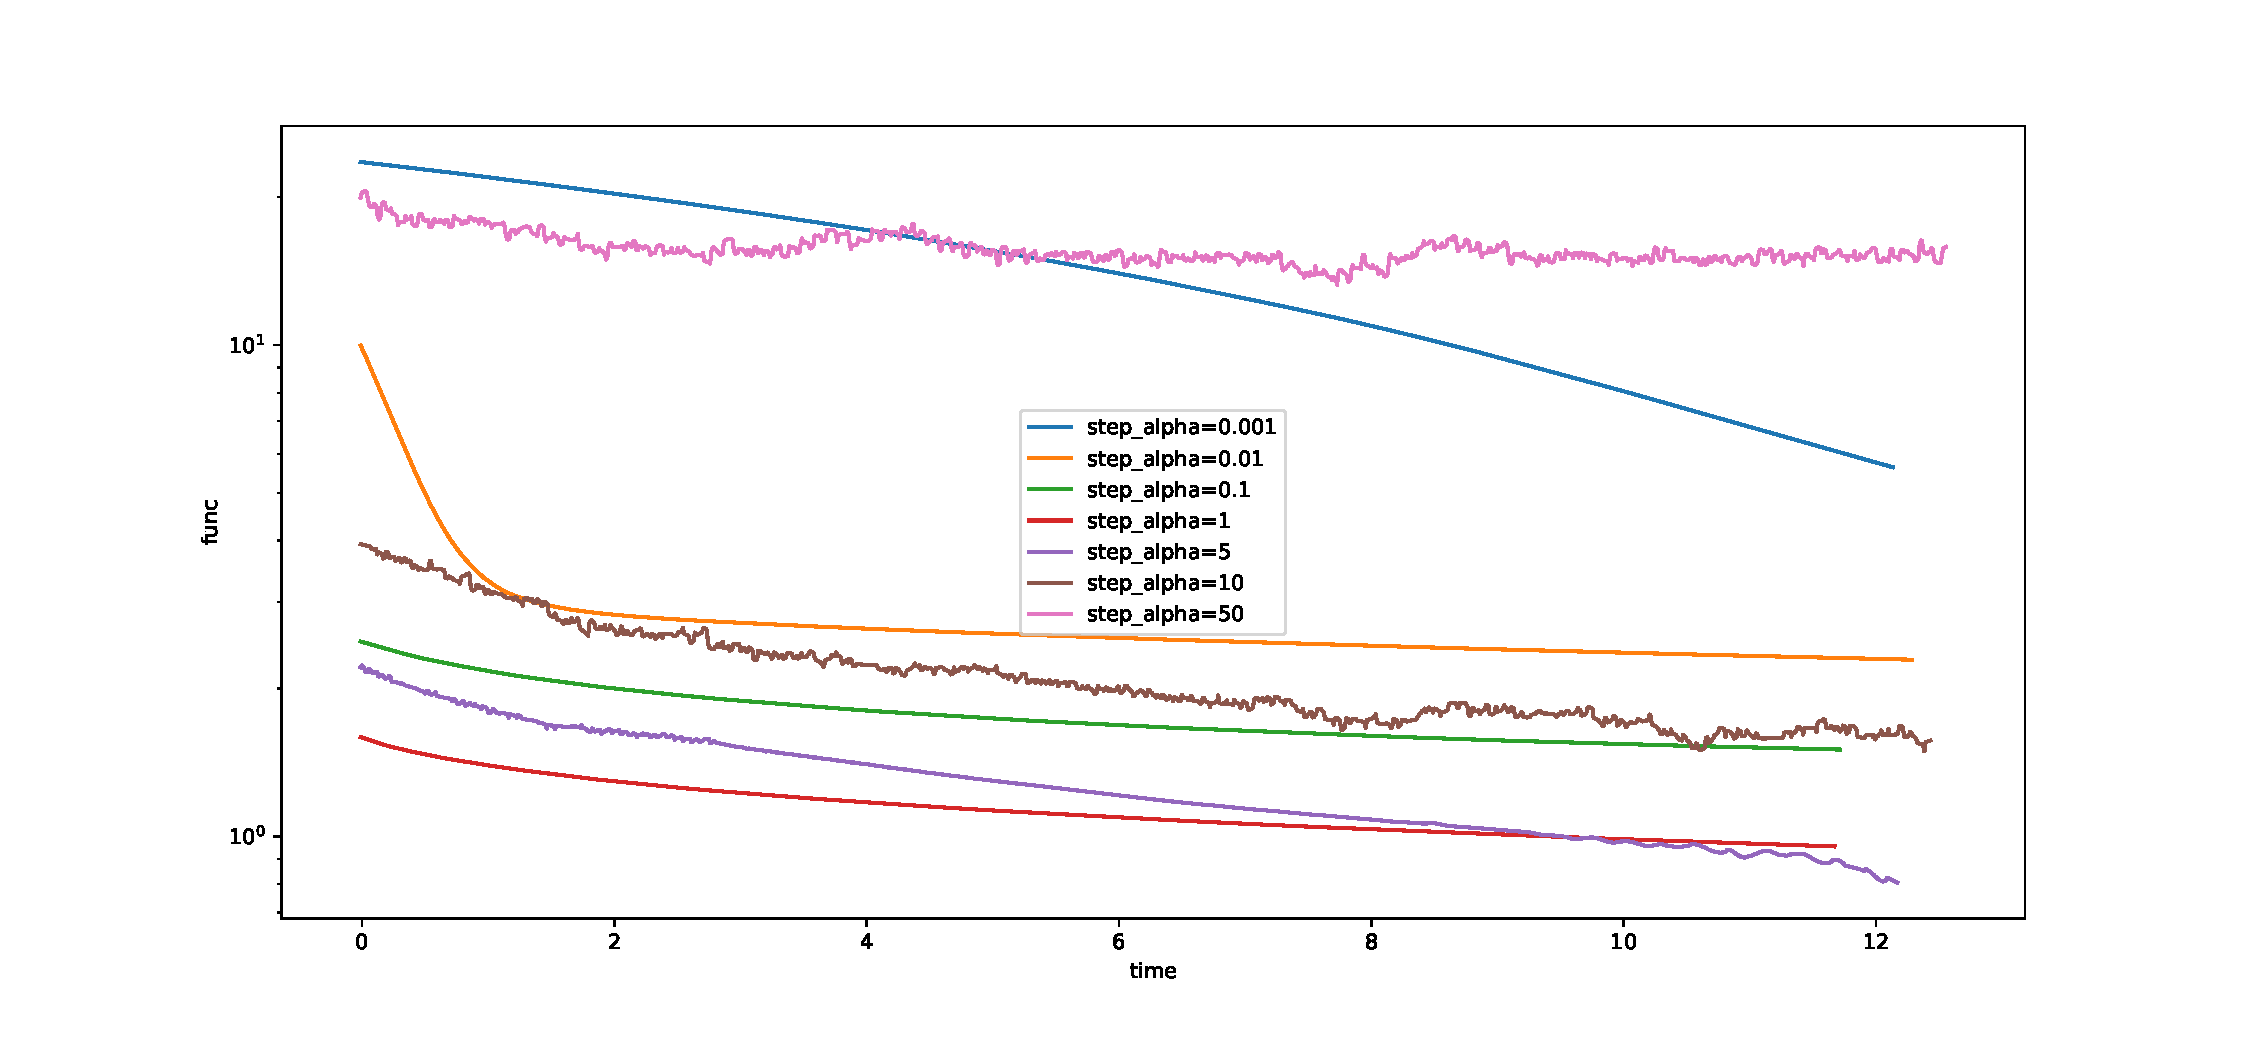
\includegraphics[width=0.5\textwidth, height=0.25\textheight]{../graphs/exp1_func_GD_alpha_time_beta=0,001.pdf}
                            
                            \caption{Зависимость значения точности (accuracy) от реального времени работы градиентного спуска} \label{exp2:gd_acc_time}
                            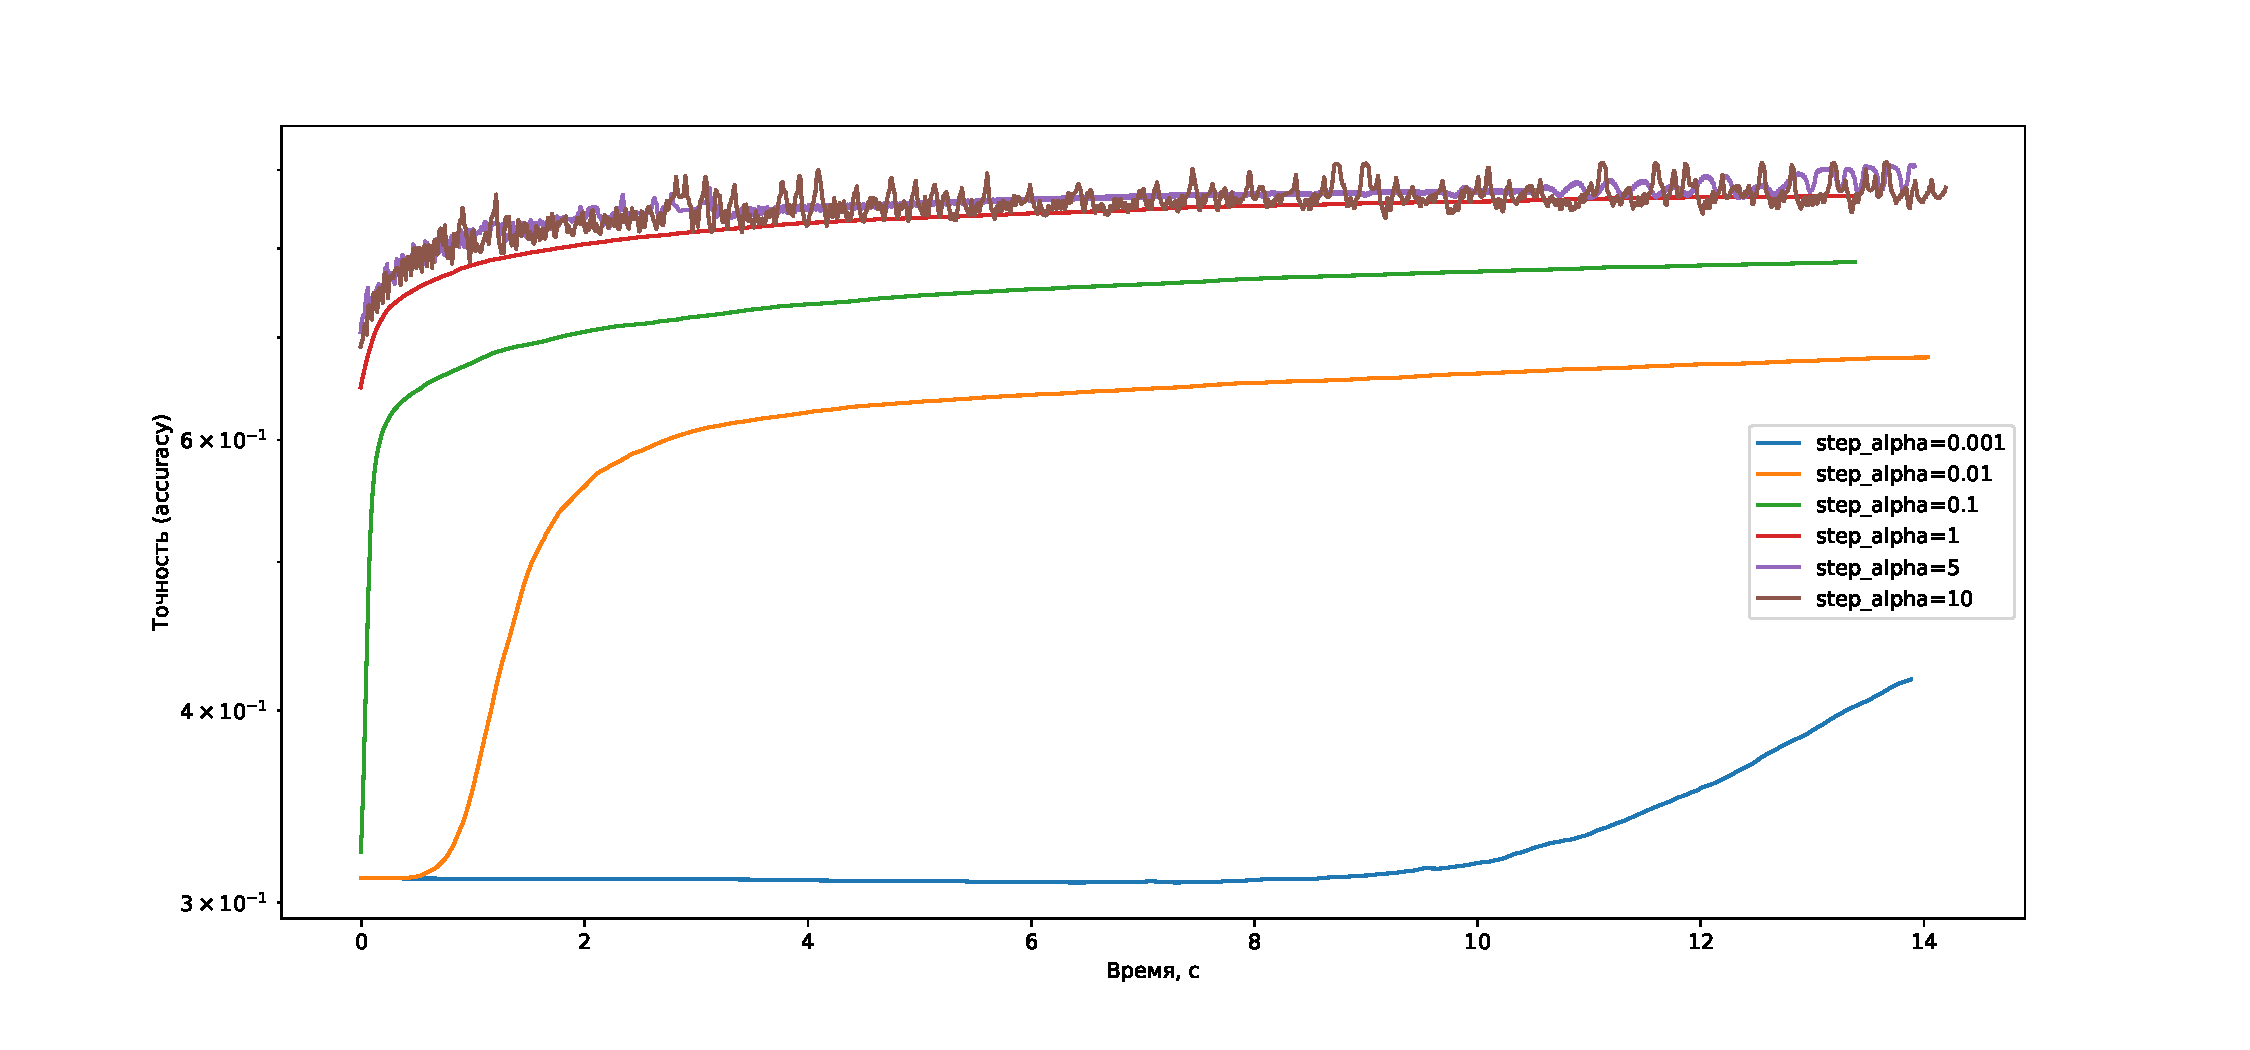
\includegraphics[width=0.5\textwidth, height=0.25\textheight]{../graphs/exp1_accuracy_GD_alpha_time_beta=0,001.pdf}
                            
                            \caption{Зависимость значения функции потерь от итерации метода градиентного спуска} \label{exp2:gd_func_iter}
                            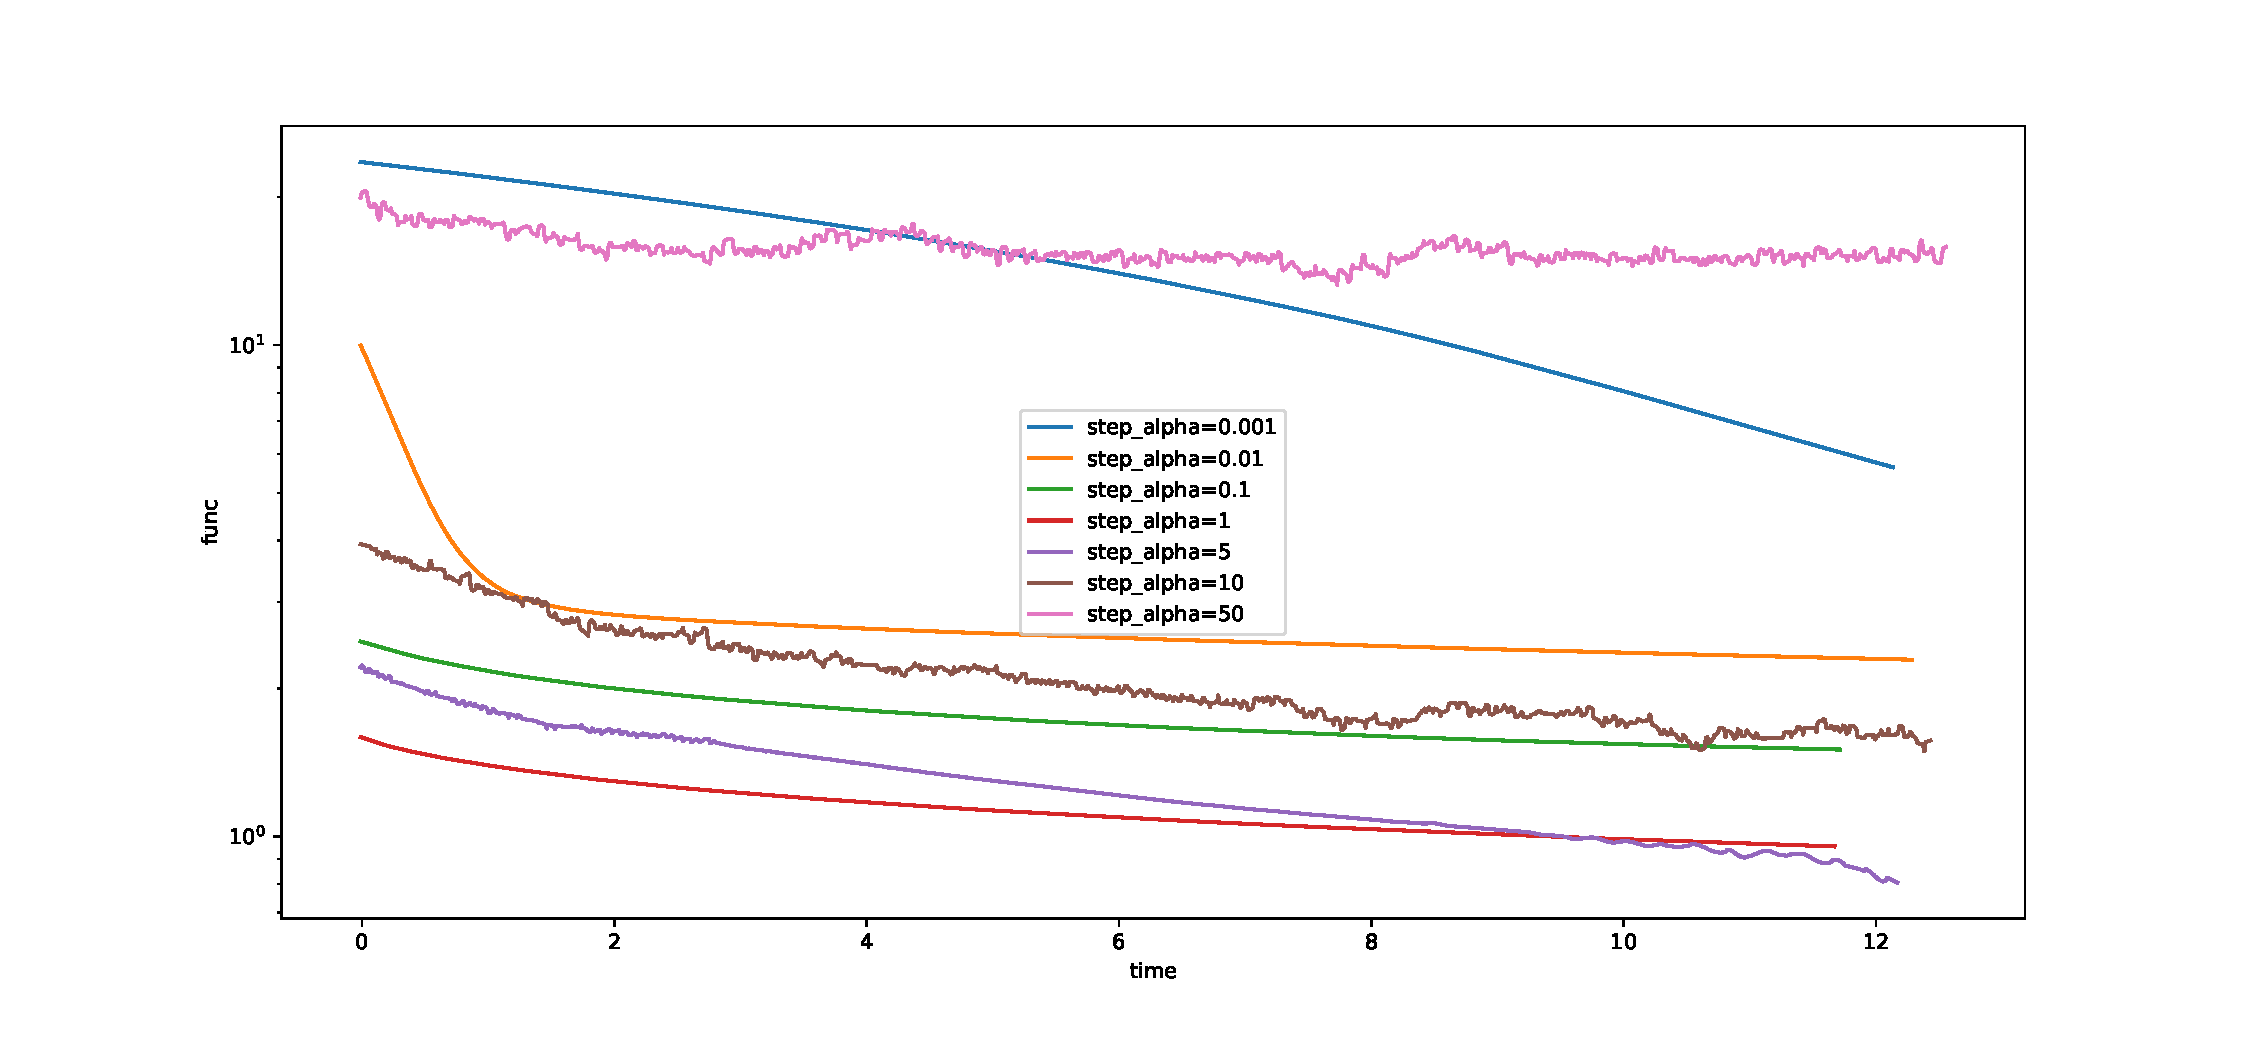
\includegraphics[width=0.5\textwidth, height=0.25\textheight]{../graphs/exp1_func_GD_alpha_time_beta=0,001.pdf}
                            
                            \caption{Зависимость значения точности (accuracy) от итерации метода градиентного спуска} \label{exp2:gd_acc_iter}
                            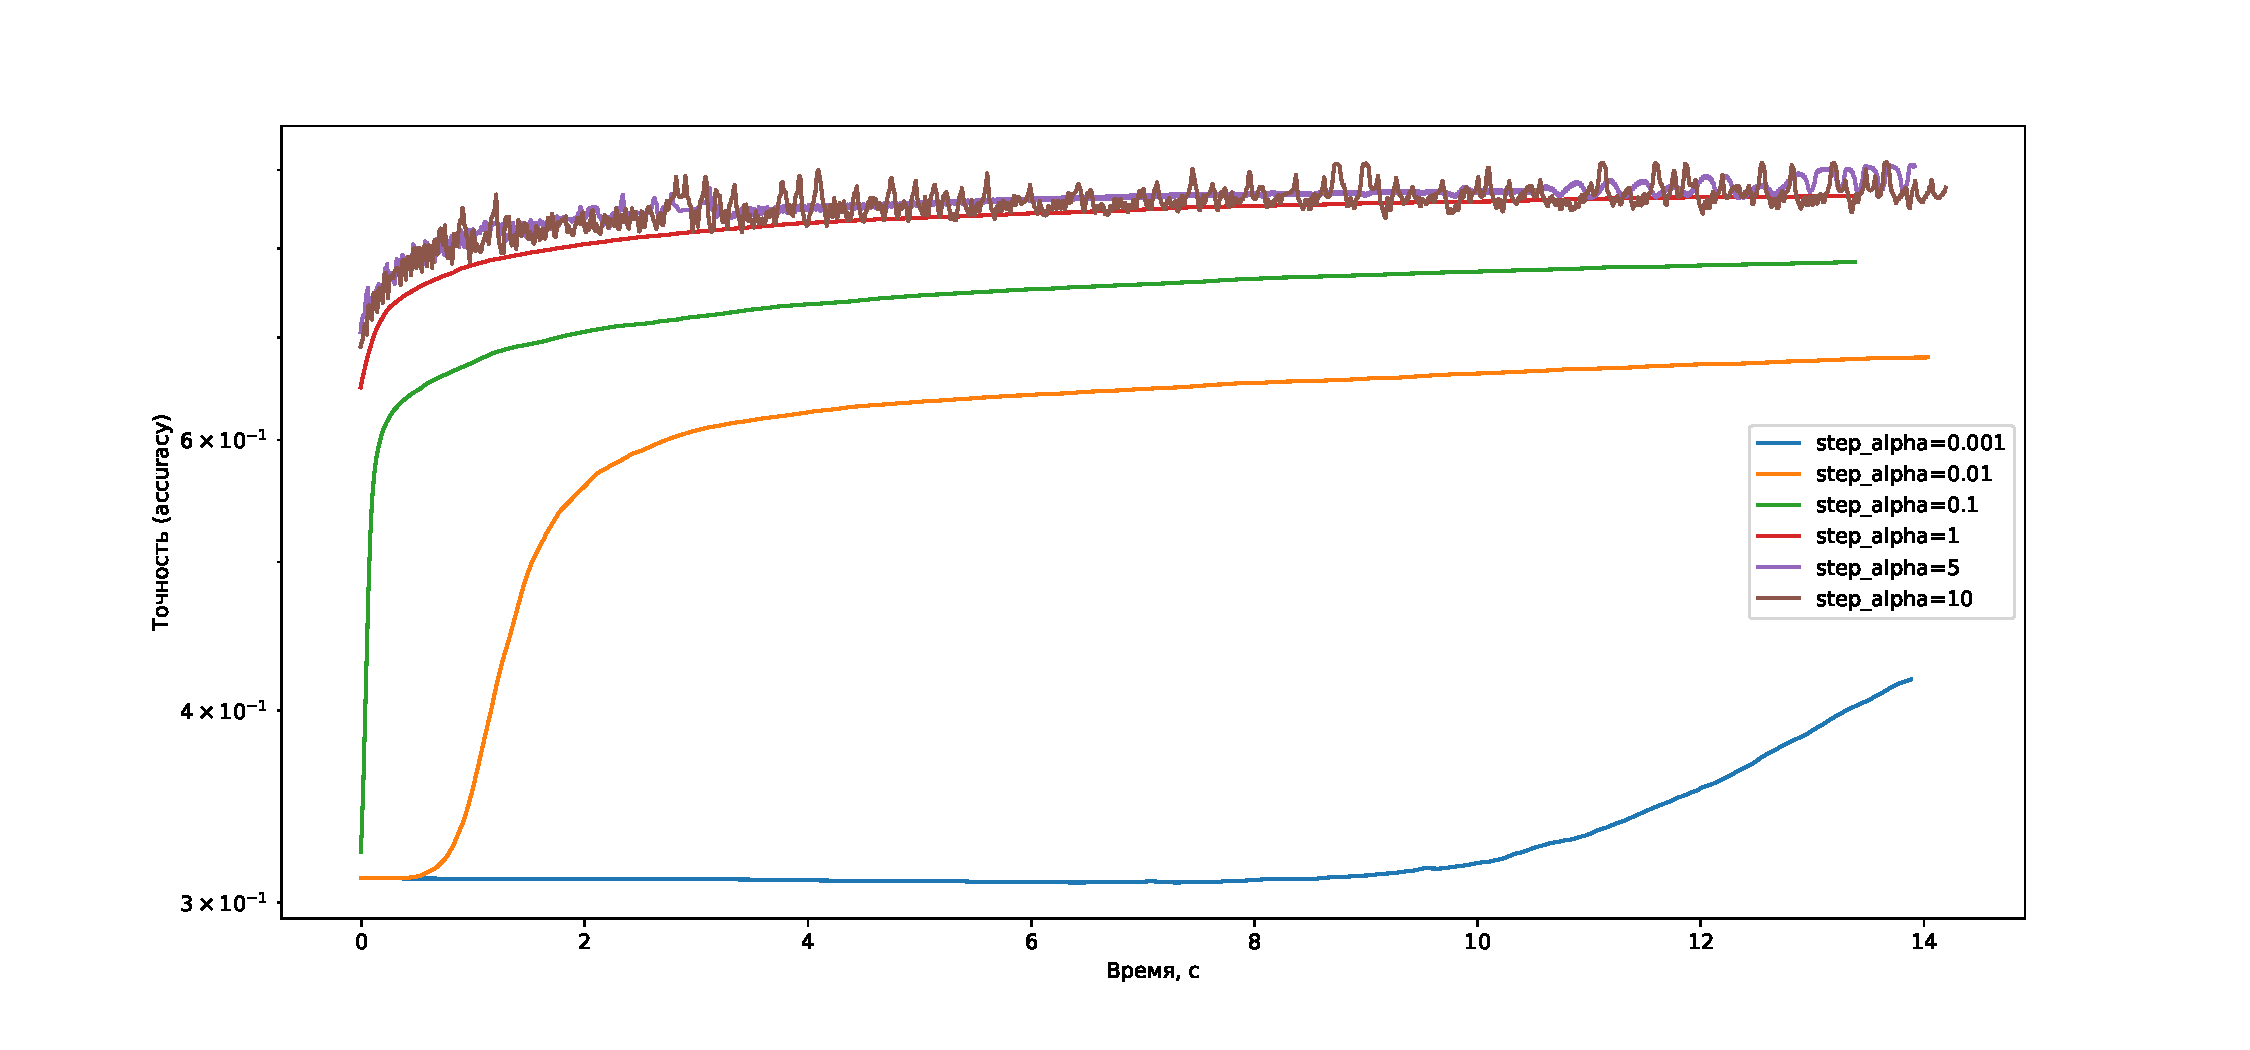
\includegraphics[width=0.5\textwidth, height=0.25\textheight]{../graphs/exp1_accuracy_GD_alpha_time_beta=0,001.pdf}
                        \end{center}
                    \end{multicols}
                \end{figure}
            
            \subsubsection{Начальное приближение $w_0$}
                Начальное приближение нужно для инициализации весов модели. В данной работе были рассмотрены следующие варианты задания $w_0$:
                \begin{itemize}
                    \item нулевой вектор
                    \item вектор с координатами из $U(0, 1)$
                    \item вектор с координатами из $U(100, 500)$
                    \item вектор с координатами из $U(1000, 5000)$
                    \item вектор с координатами из $U(10000, 50000)$
                    \item вектор с координатами из $N(0, 1)$
                    \item вектор с координатами из $N(0.5, 0.5)$
                \end{itemize}
                Графики зависимостей \ref{exp:dependencies} представлены на рис.  \ref{exp3:gd_func_time}, \ref{exp3:gd_acc_time}, \ref{exp3:gd_func_iter}, \ref{exp3:gd_acc_iter}.
                \begin{figure}[H] \label{exp1}
                    \begin{multicols}{2}
                        \begin{center}
                            \caption{Зависимость значения функции потерь от реального времени работы стохастического градиентного спуска} \label{exp3:gd_func_time}
                            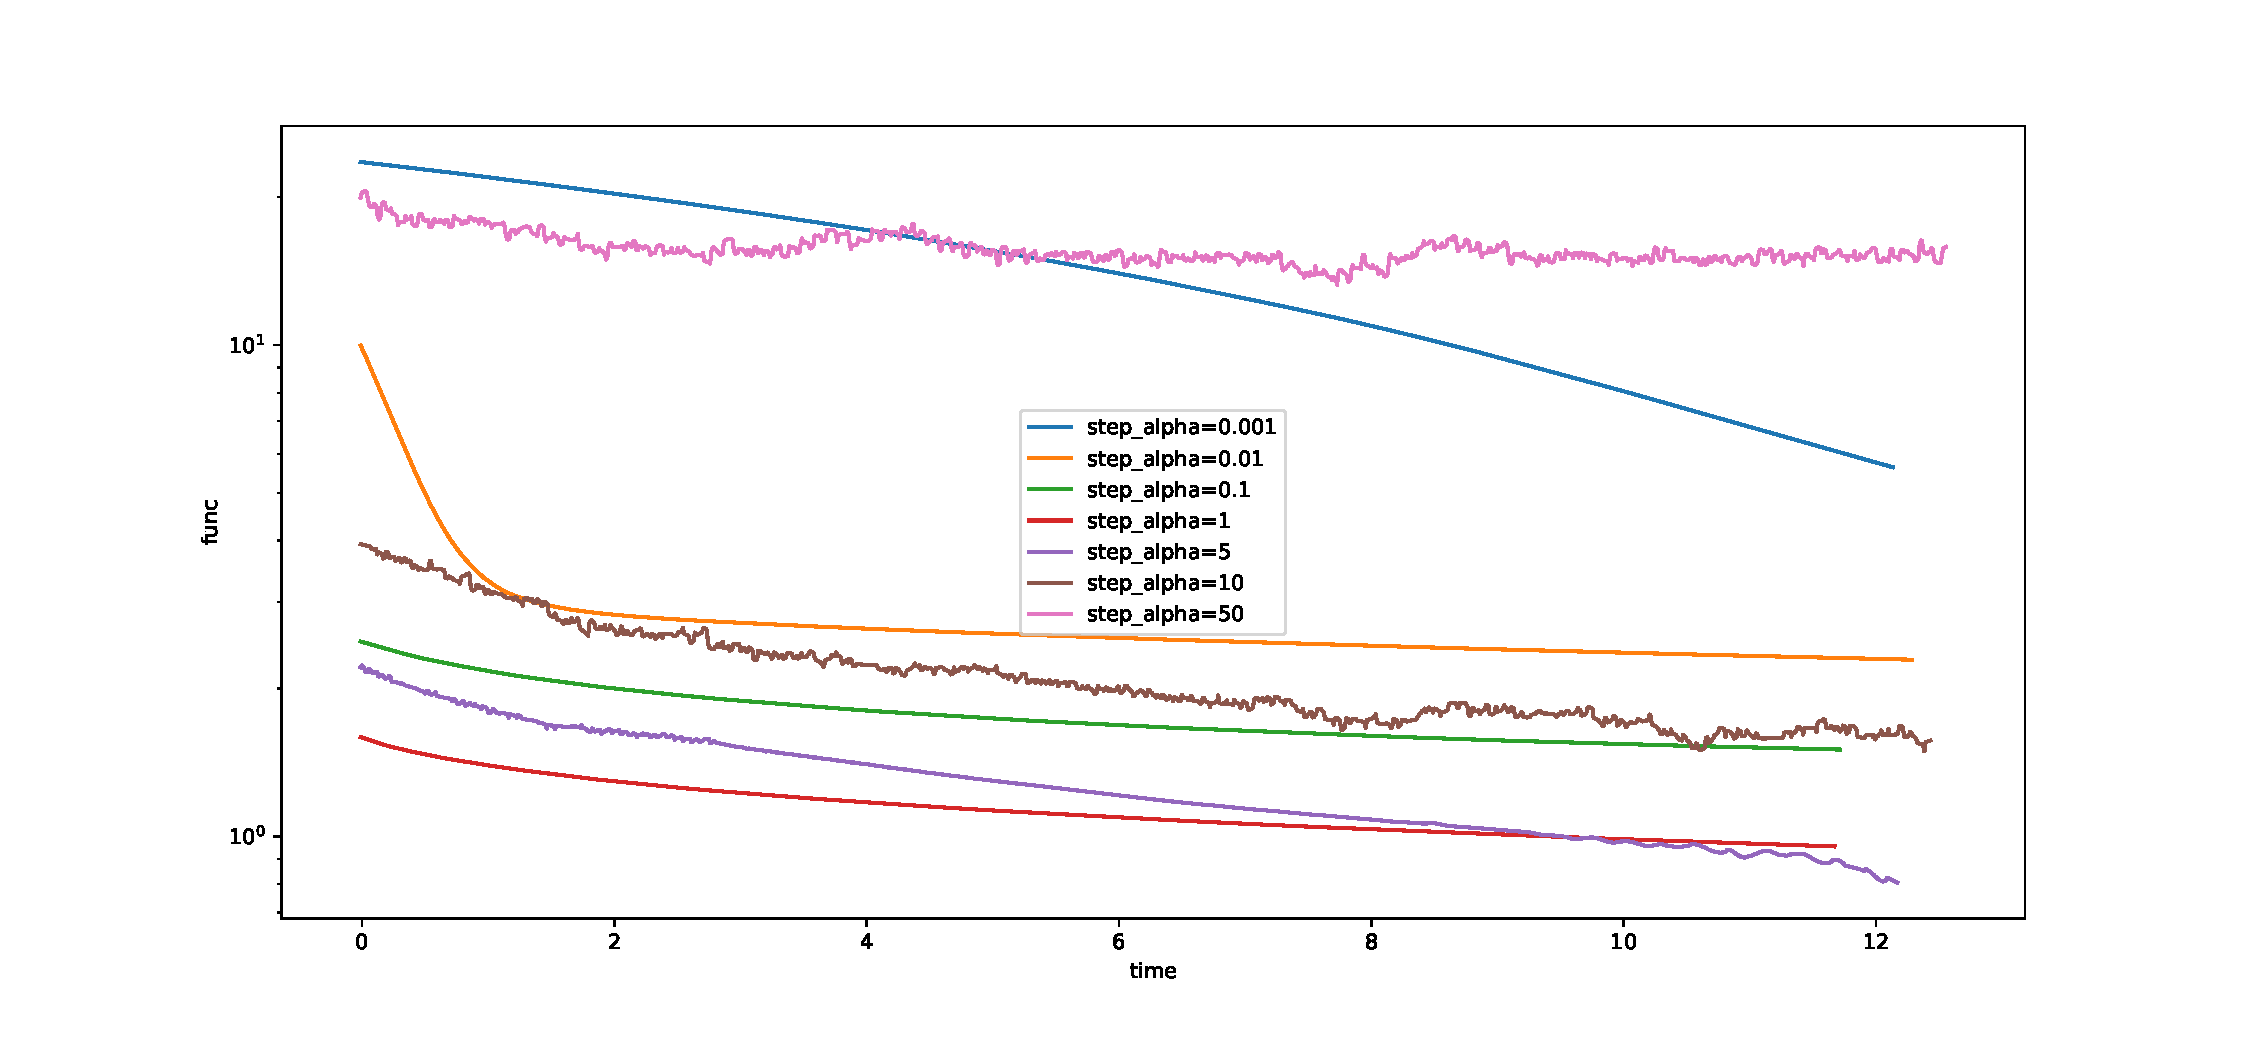
\includegraphics[width=0.5\textwidth, height=0.25\textheight]{../graphs/exp1_func_GD_alpha_time_beta=0,001.pdf}
                            
                            \caption{Зависимость значения точности (accuracy) от реального времени работы стохастического градиентного спуска} \label{exp3:gd_acc_time}
                            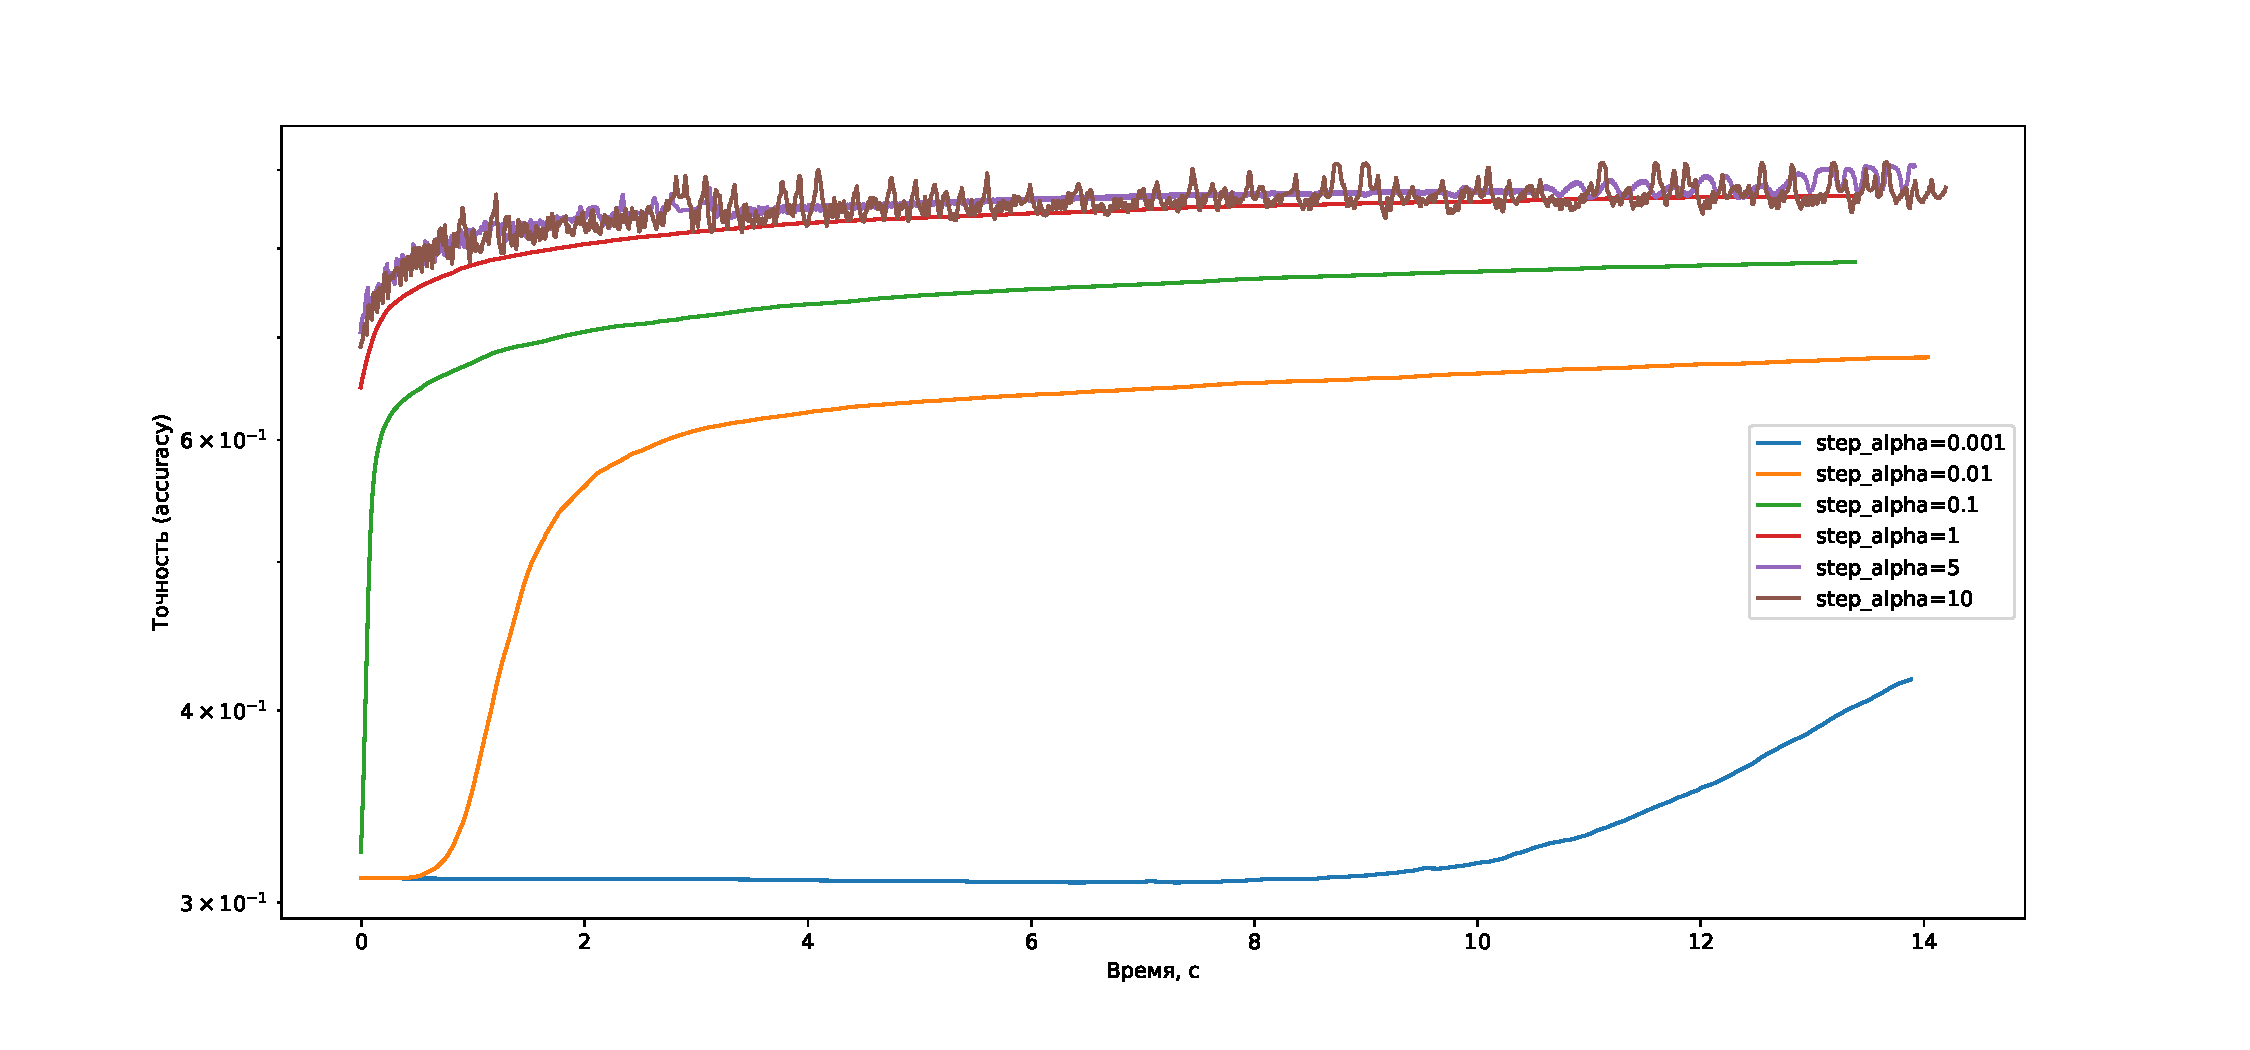
\includegraphics[width=0.5\textwidth, height=0.25\textheight]{../graphs/exp1_accuracy_GD_alpha_time_beta=0,001.pdf}
                            
                            \caption{Зависимость значения функции потерь от итерации метода стохастического градиентного спуска} \label{exp3:gd_func_iter}
                            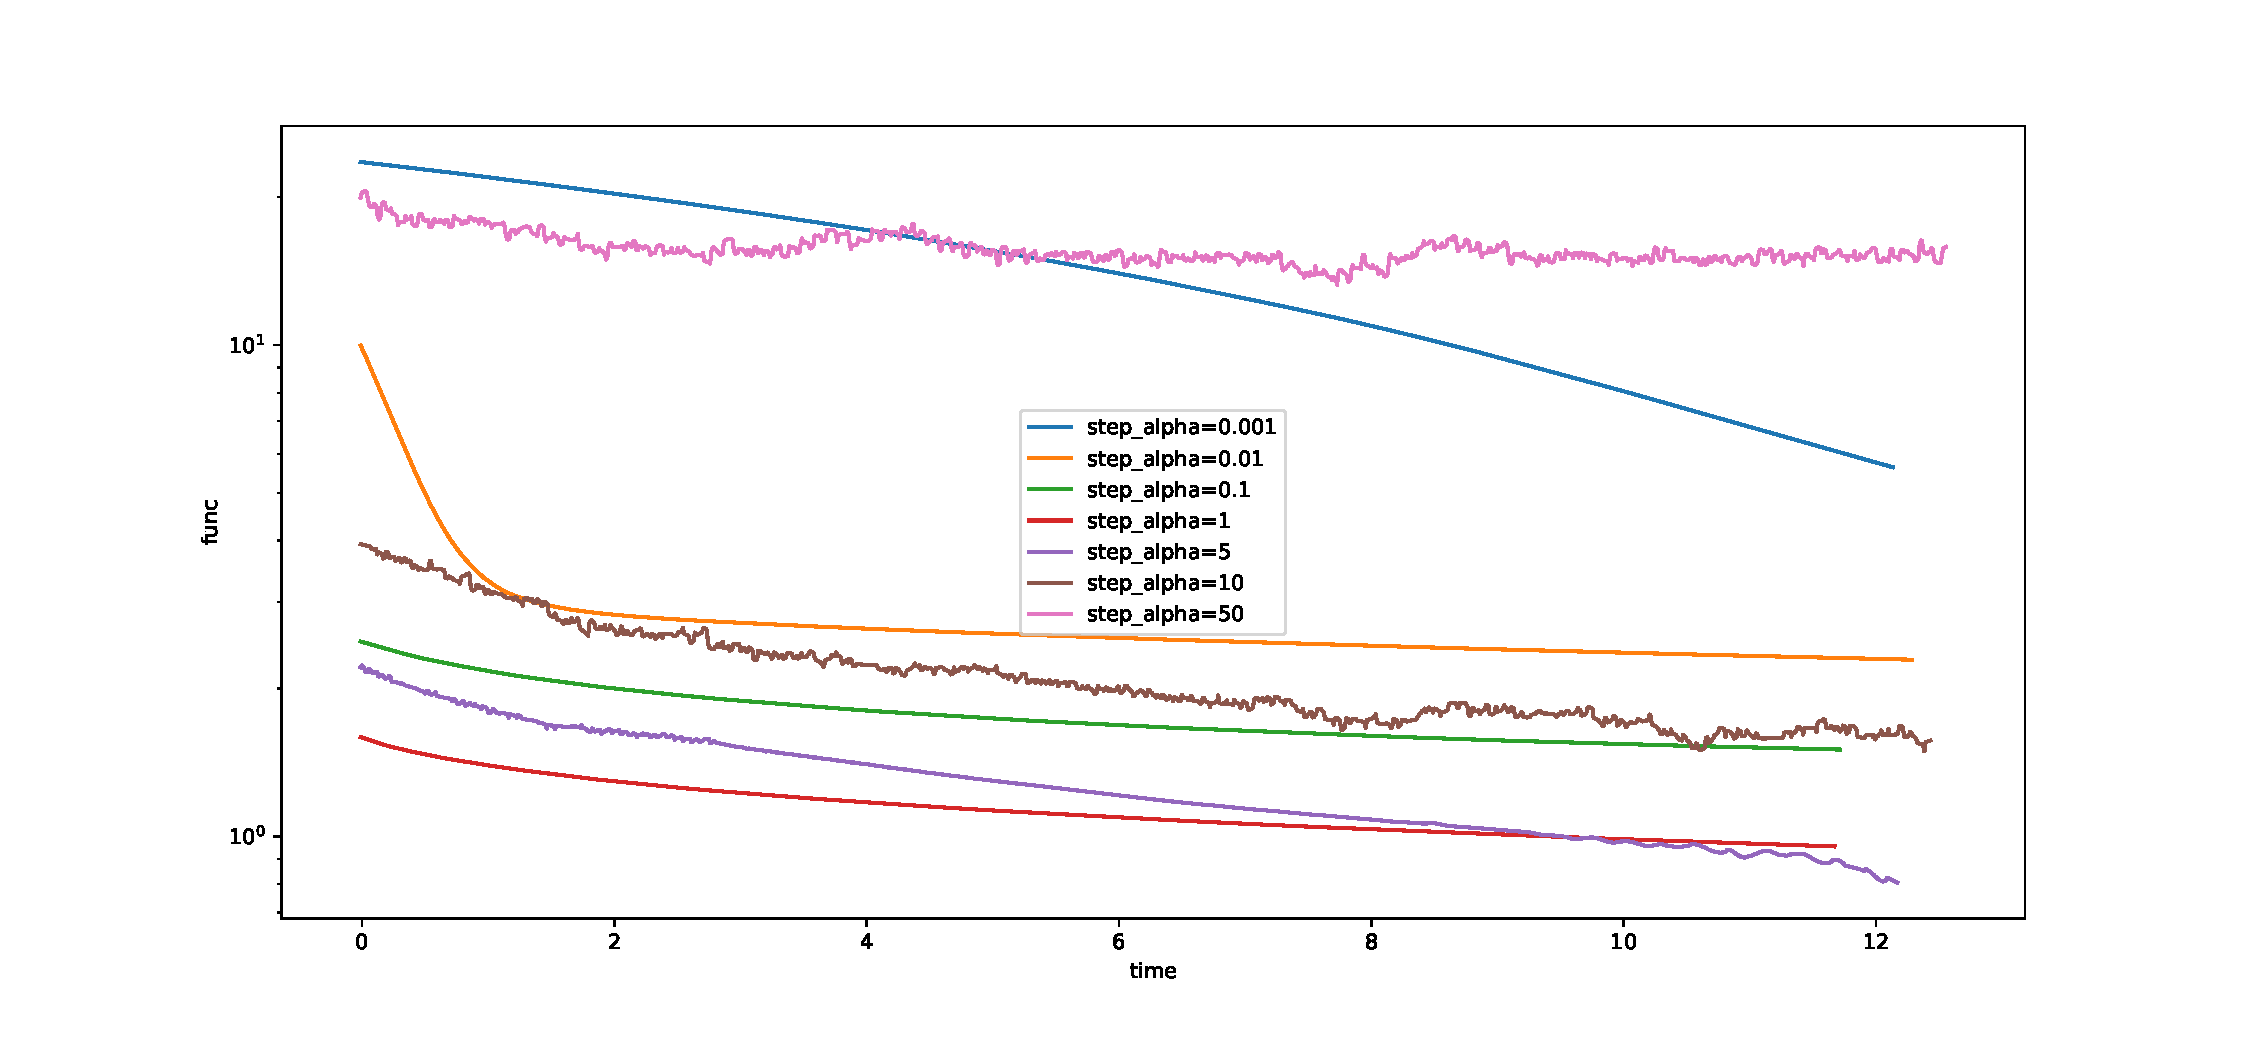
\includegraphics[width=0.5\textwidth, height=0.25\textheight]{../graphs/exp1_func_GD_alpha_time_beta=0,001.pdf}
                            
                            \caption{Зависимость значения точности (accuracy) от итерации метода стохастического градиентного спуска} \label{exp3:gd_acc_iter}
                            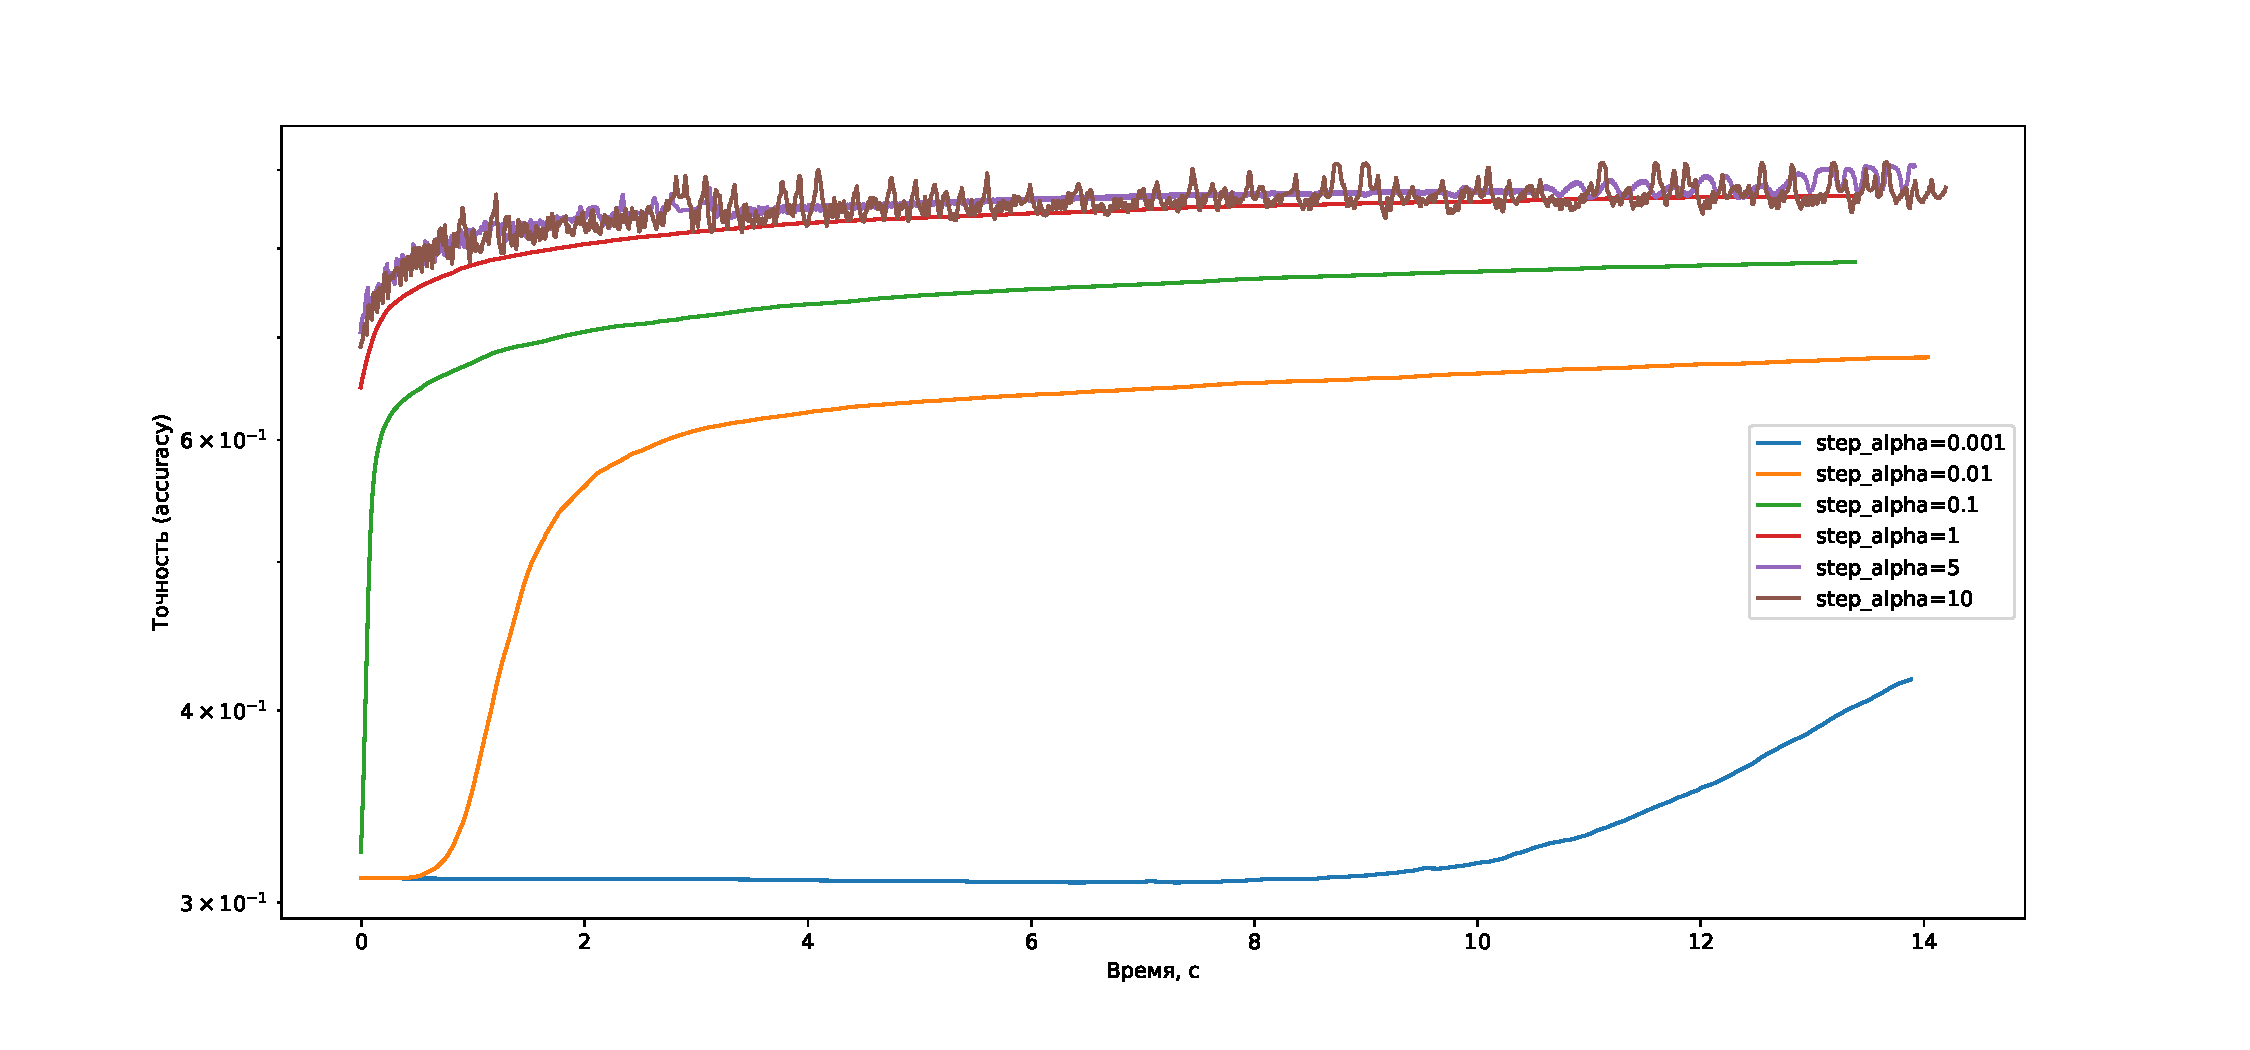
\includegraphics[width=0.5\textwidth, height=0.25\textheight]{../graphs/exp1_accuracy_GD_alpha_time_beta=0,001.pdf}
                        \end{center}
                    \end{multicols}
                \end{figure}
            
            
       \subsection{Исследование поведения стохастического градиентного спуска}
            Обновления весов модели при использовании стохастического градиетного спуска происходит по следующей формуле:
            \begin{equation}\label{exp1:weight_upd_sgd}
            w_t = w_{t-1} - \frac{\alpha}{t^\beta} \times \frac{1}{|I|} \times \sum_{i \in I}\nabla_{w}\mathcal{L}(x_i, y_i|w_{t-1}),
            \end{equation}
            где $t$ - номер итерации, $\beta$ - \textbf{step\_beta}, $I$ - некоторое подможнество индексов тренировочной выборки,  $\nabla_{w}\mathcal{L}(x_i, y_i|w_{t-1})$ - градиент функции потерь.
            \subsubsection{Параметр размера шага \textbf{step\_alpha}}
            Параметр \textbf{step\_alpha $(\alpha)$} используется в стохастическом градиентном спуске при обновлении весов в формуле \ref{exp1:weight_upd_sgd}.
            Рассмотрим следующие зависимости при разных значениях параметра \textbf{step\_alpha}:
            \begin{enumerate}\label{exp:dependencies_sgd}
                \item зависимость значения функции потерь от реального времени работы метода
                \item зависимость точности (accuracy) от реального времени работы метода
                \item зависимость значения функции потерь от эпохи метода
                \item зависимость точности (accuracy) от эпохи метода
            \end{enumerate}
            Соответствующие графики приведены на: рис. \ref{exp1:sgd_func_time}, \ref{exp1:sgd_acc_time}, \ref{exp1:sgd_func_iter}, \ref{exp1:sgd_acc_iter}.
            
            \begin{figure}[H] \label{exp1}
                \begin{multicols}{2}
                    \begin{center}
                        \caption{Зависимость значения функции потерь от реального времени работы градиентного спуска} \label{exp1:sgd_func_time}
                        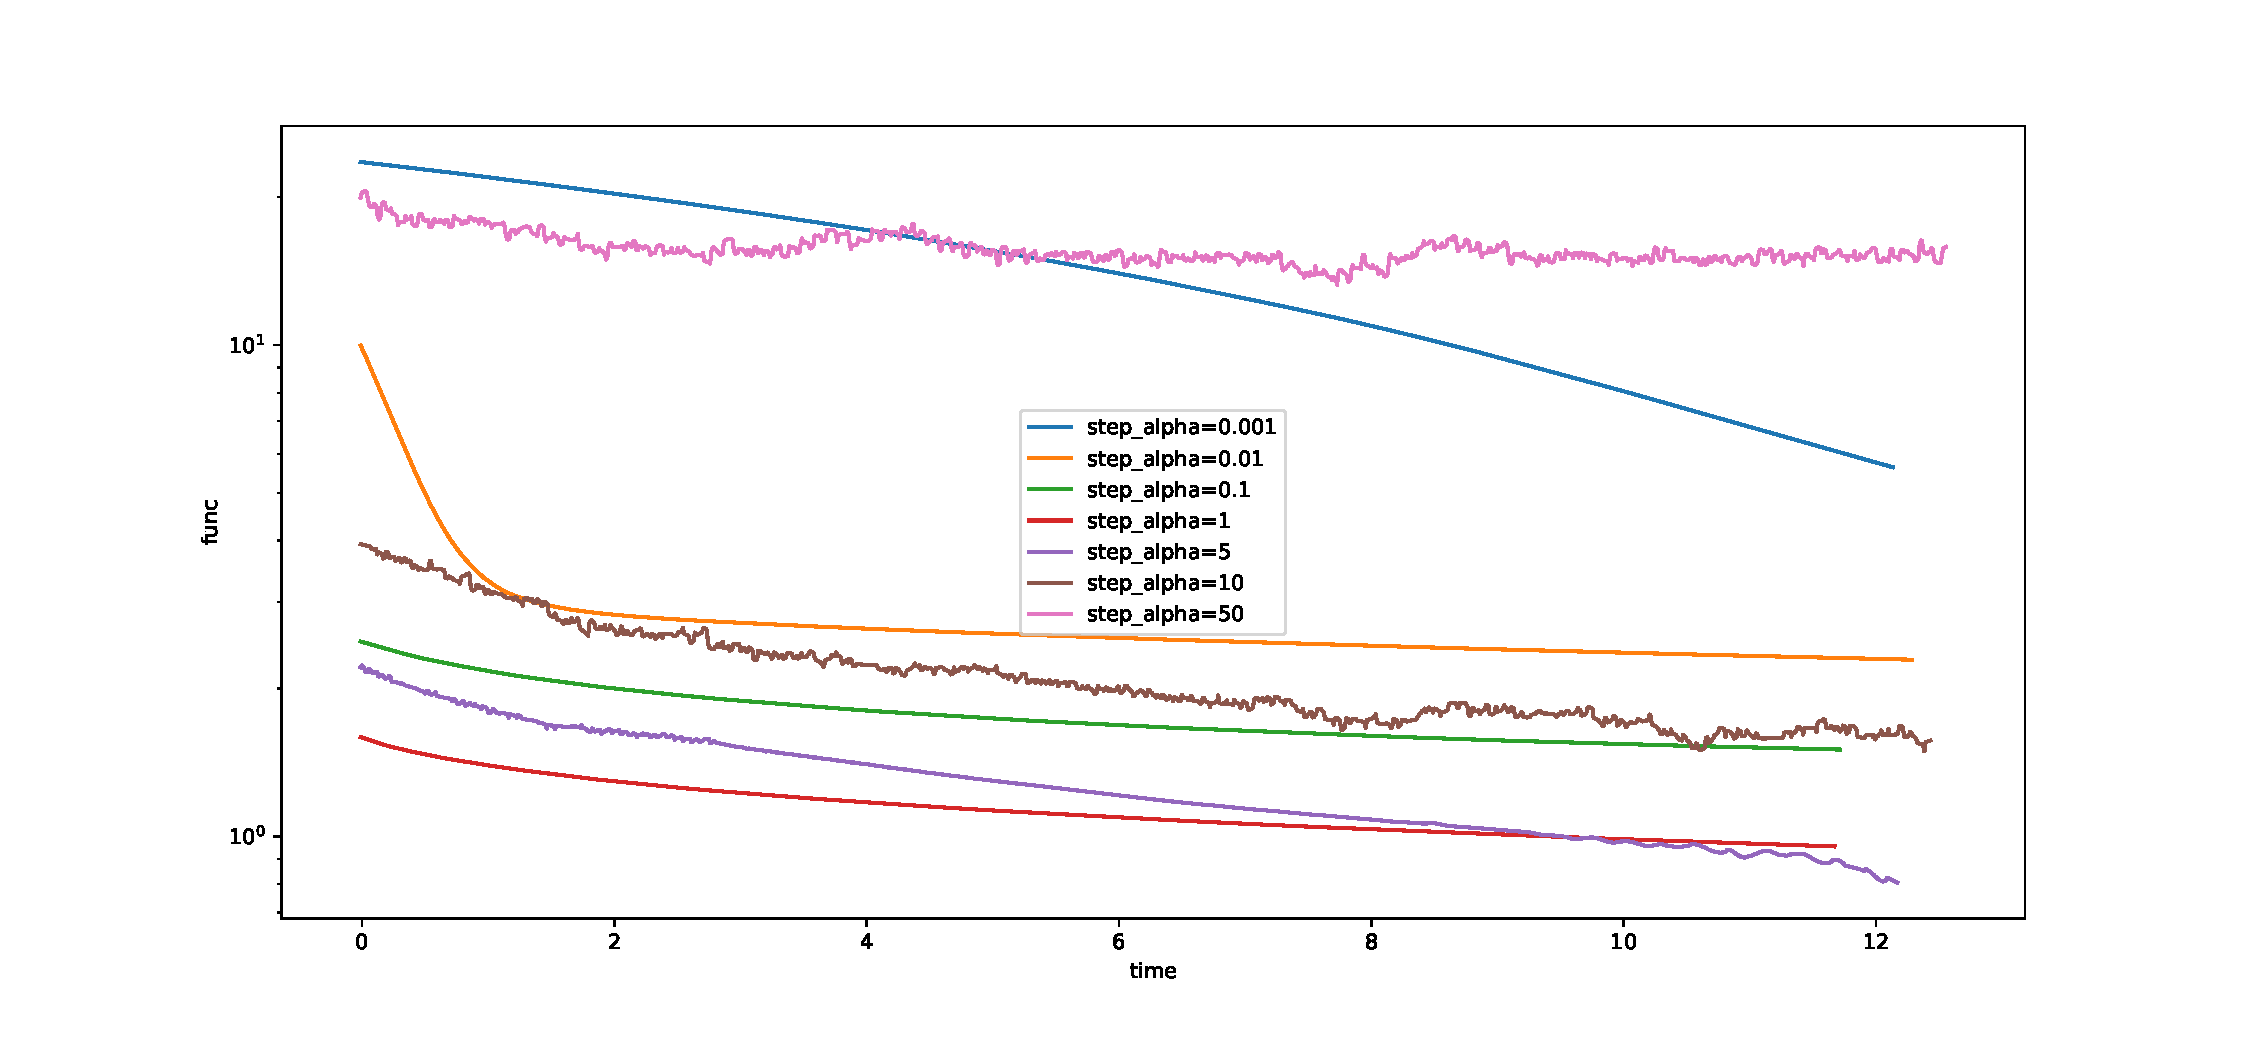
\includegraphics[width=0.5\textwidth, height=0.25\textheight]{../graphs/exp1_func_GD_alpha_time_beta=0,001.pdf}
                        
                        \caption{Зависимость значения точности (accuracy) от реального времени работы градиентного спуска} \label{exp1:sgd_acc_time}
                        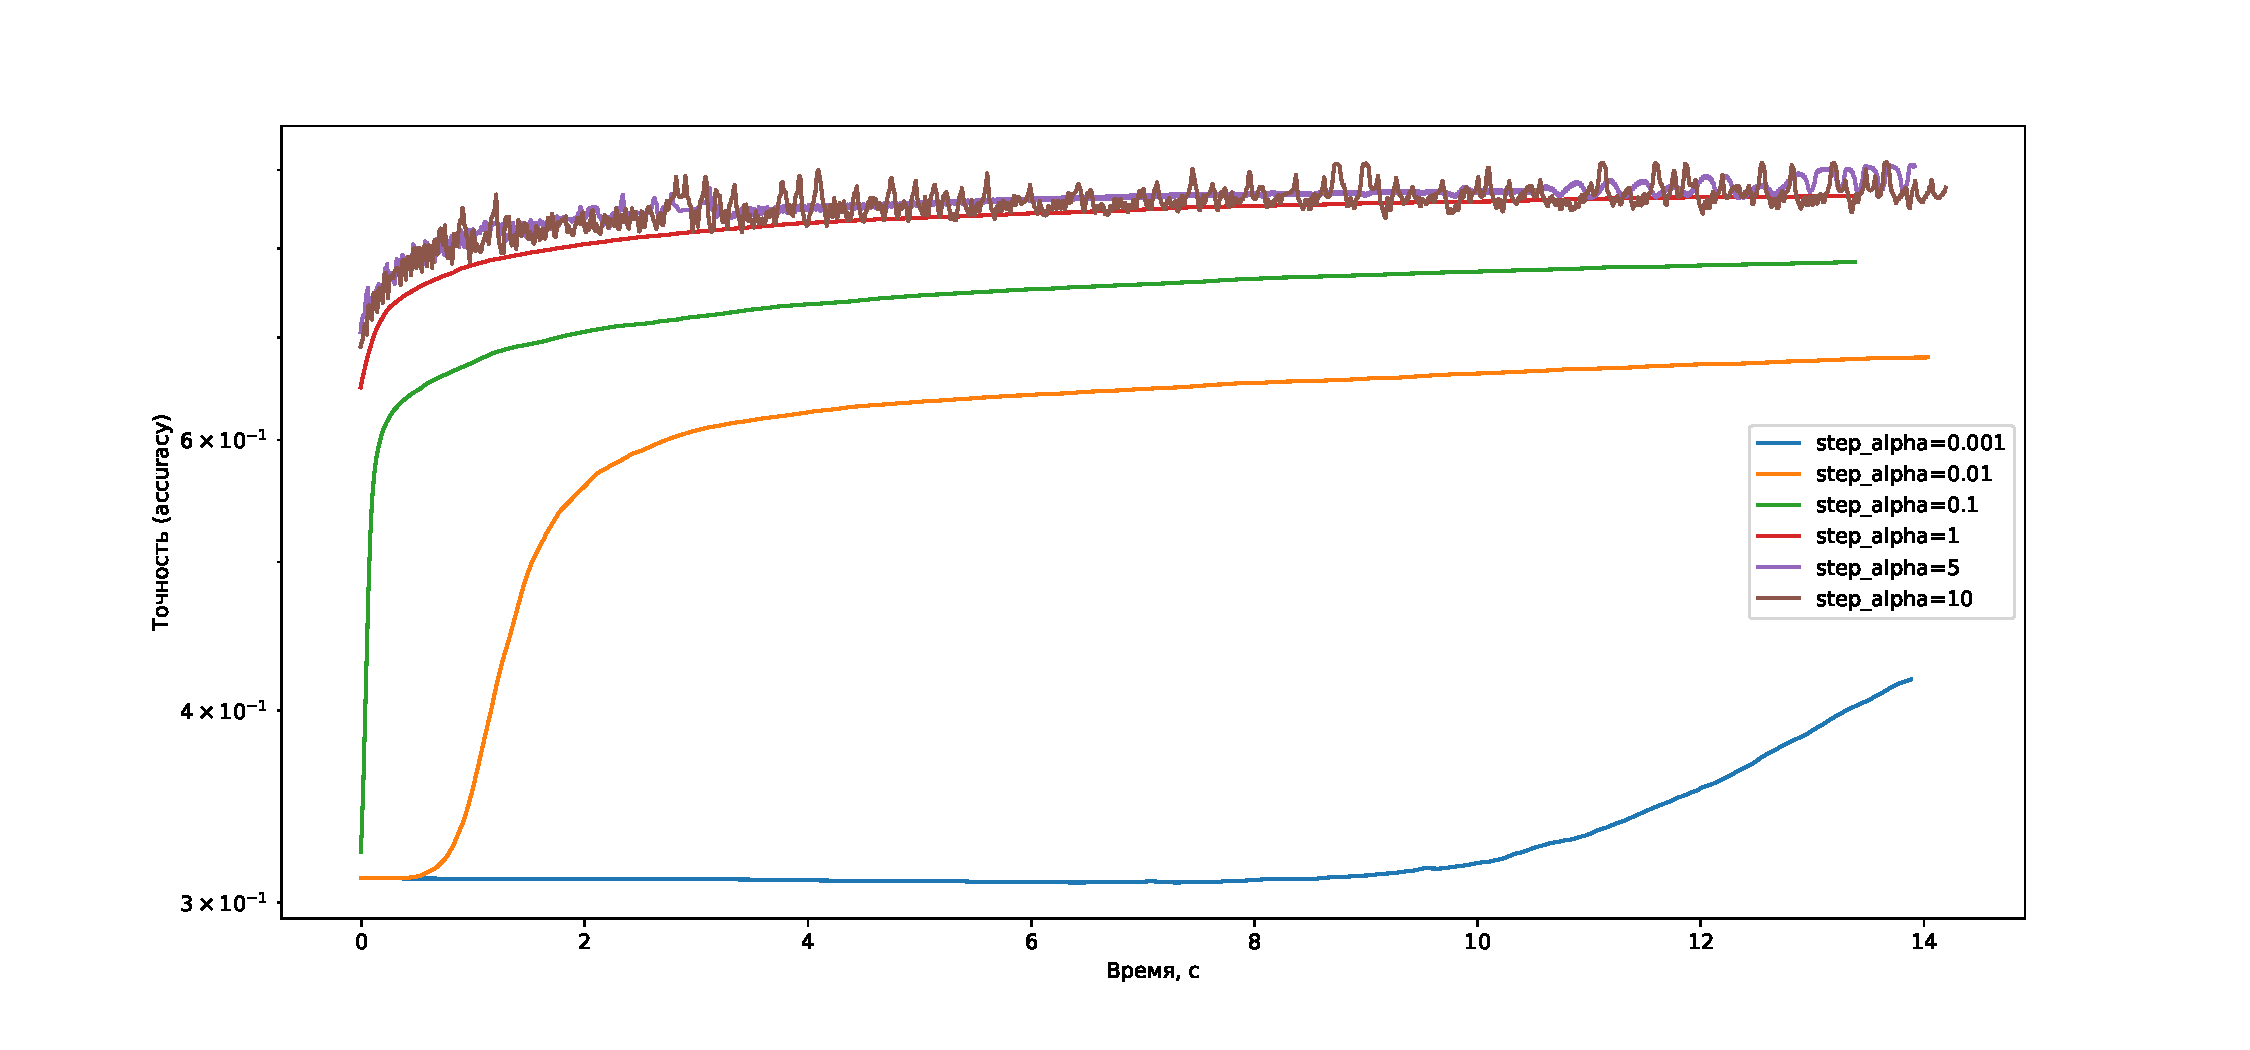
\includegraphics[width=0.5\textwidth, height=0.25\textheight]{../graphs/exp1_accuracy_GD_alpha_time_beta=0,001.pdf}
                        
                        \caption{Зависимость значения функции потерь от эпохи метода градиентного спуска} \label{exp1:sgd_func_iter}
                        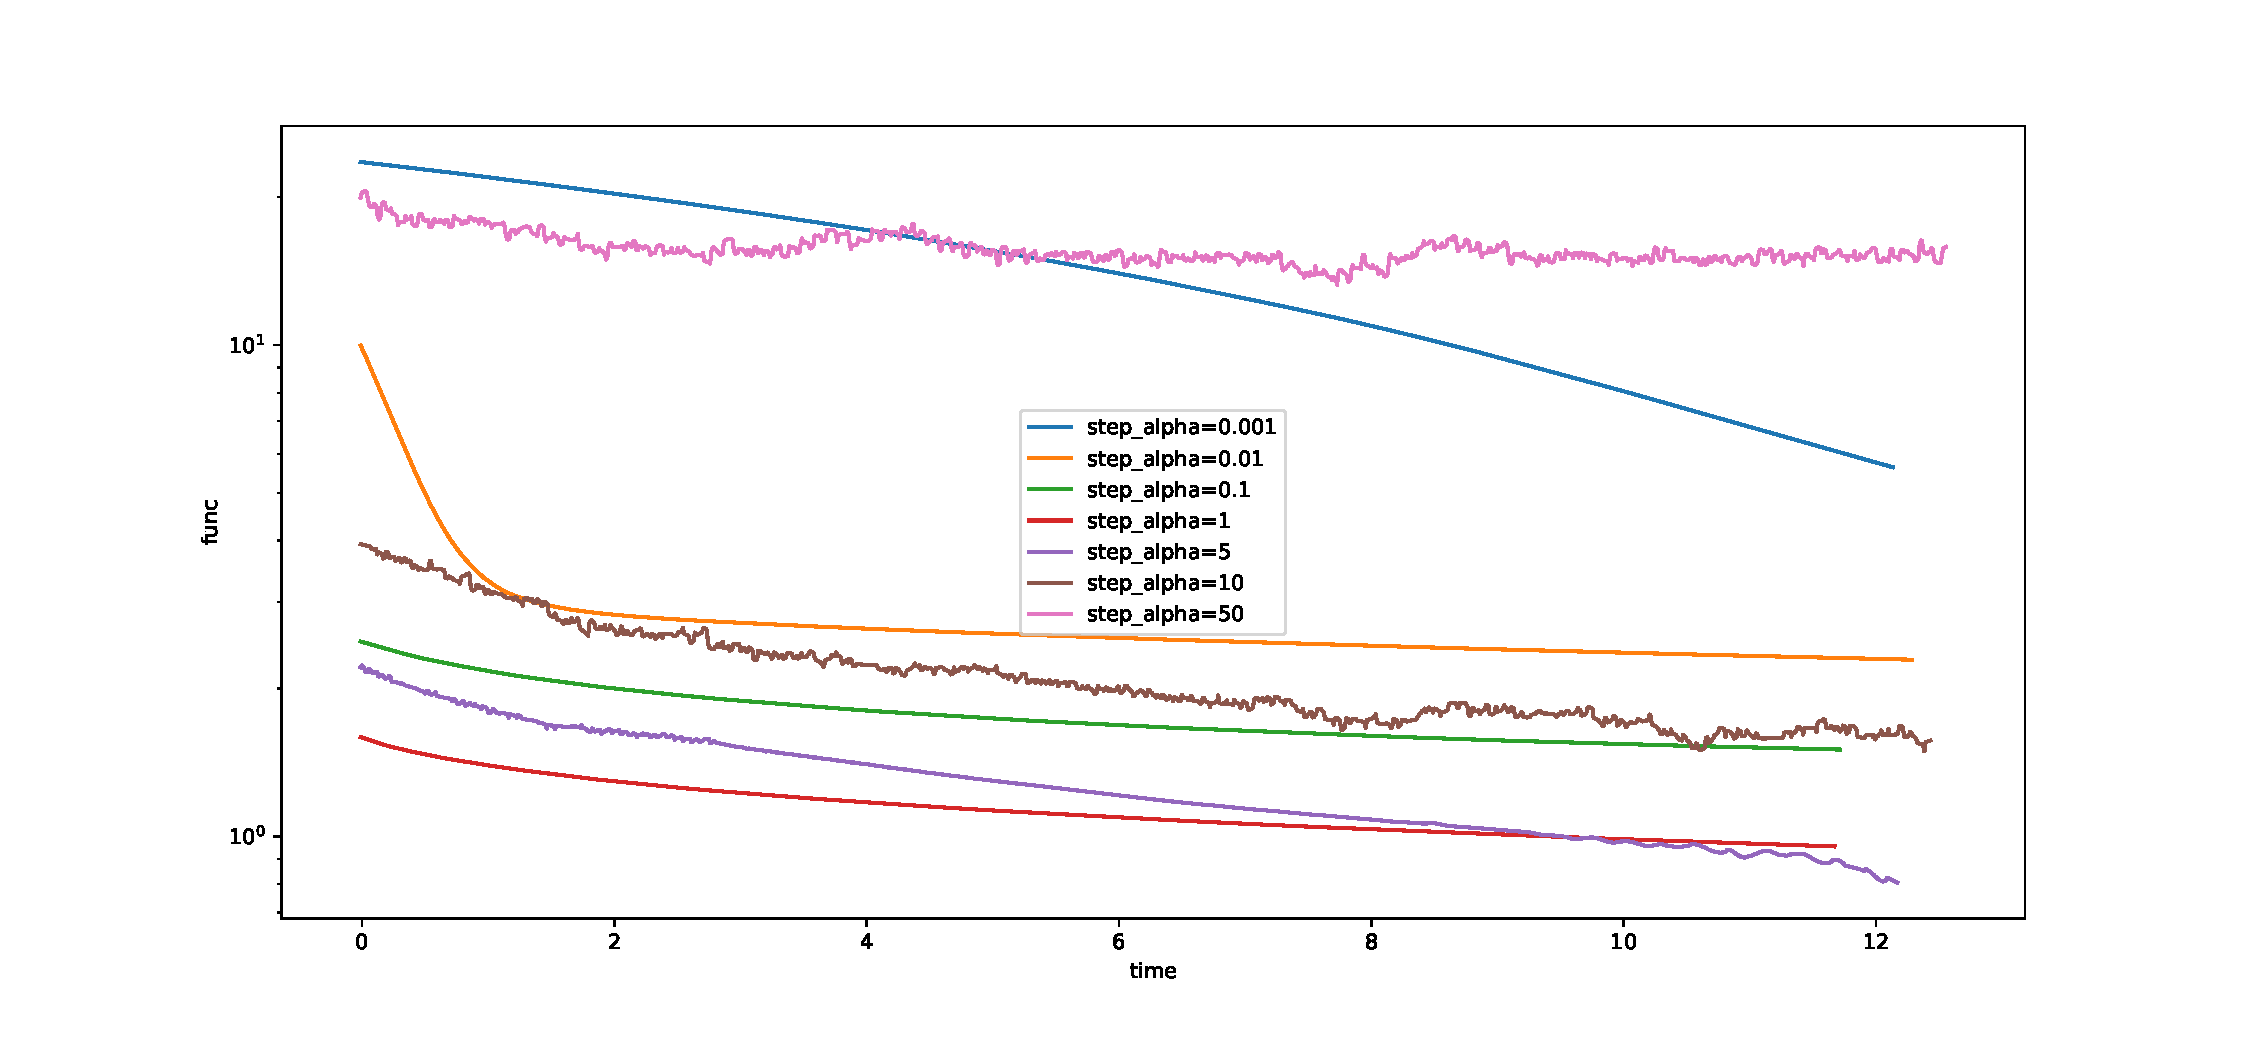
\includegraphics[width=0.5\textwidth, height=0.25\textheight]{../graphs/exp1_func_GD_alpha_time_beta=0,001.pdf}
                        
                        \caption{Зависимость значения точности (accuracy) от эпохи метода градиентного спуска} \label{exp1:sgd_acc_iter}
                        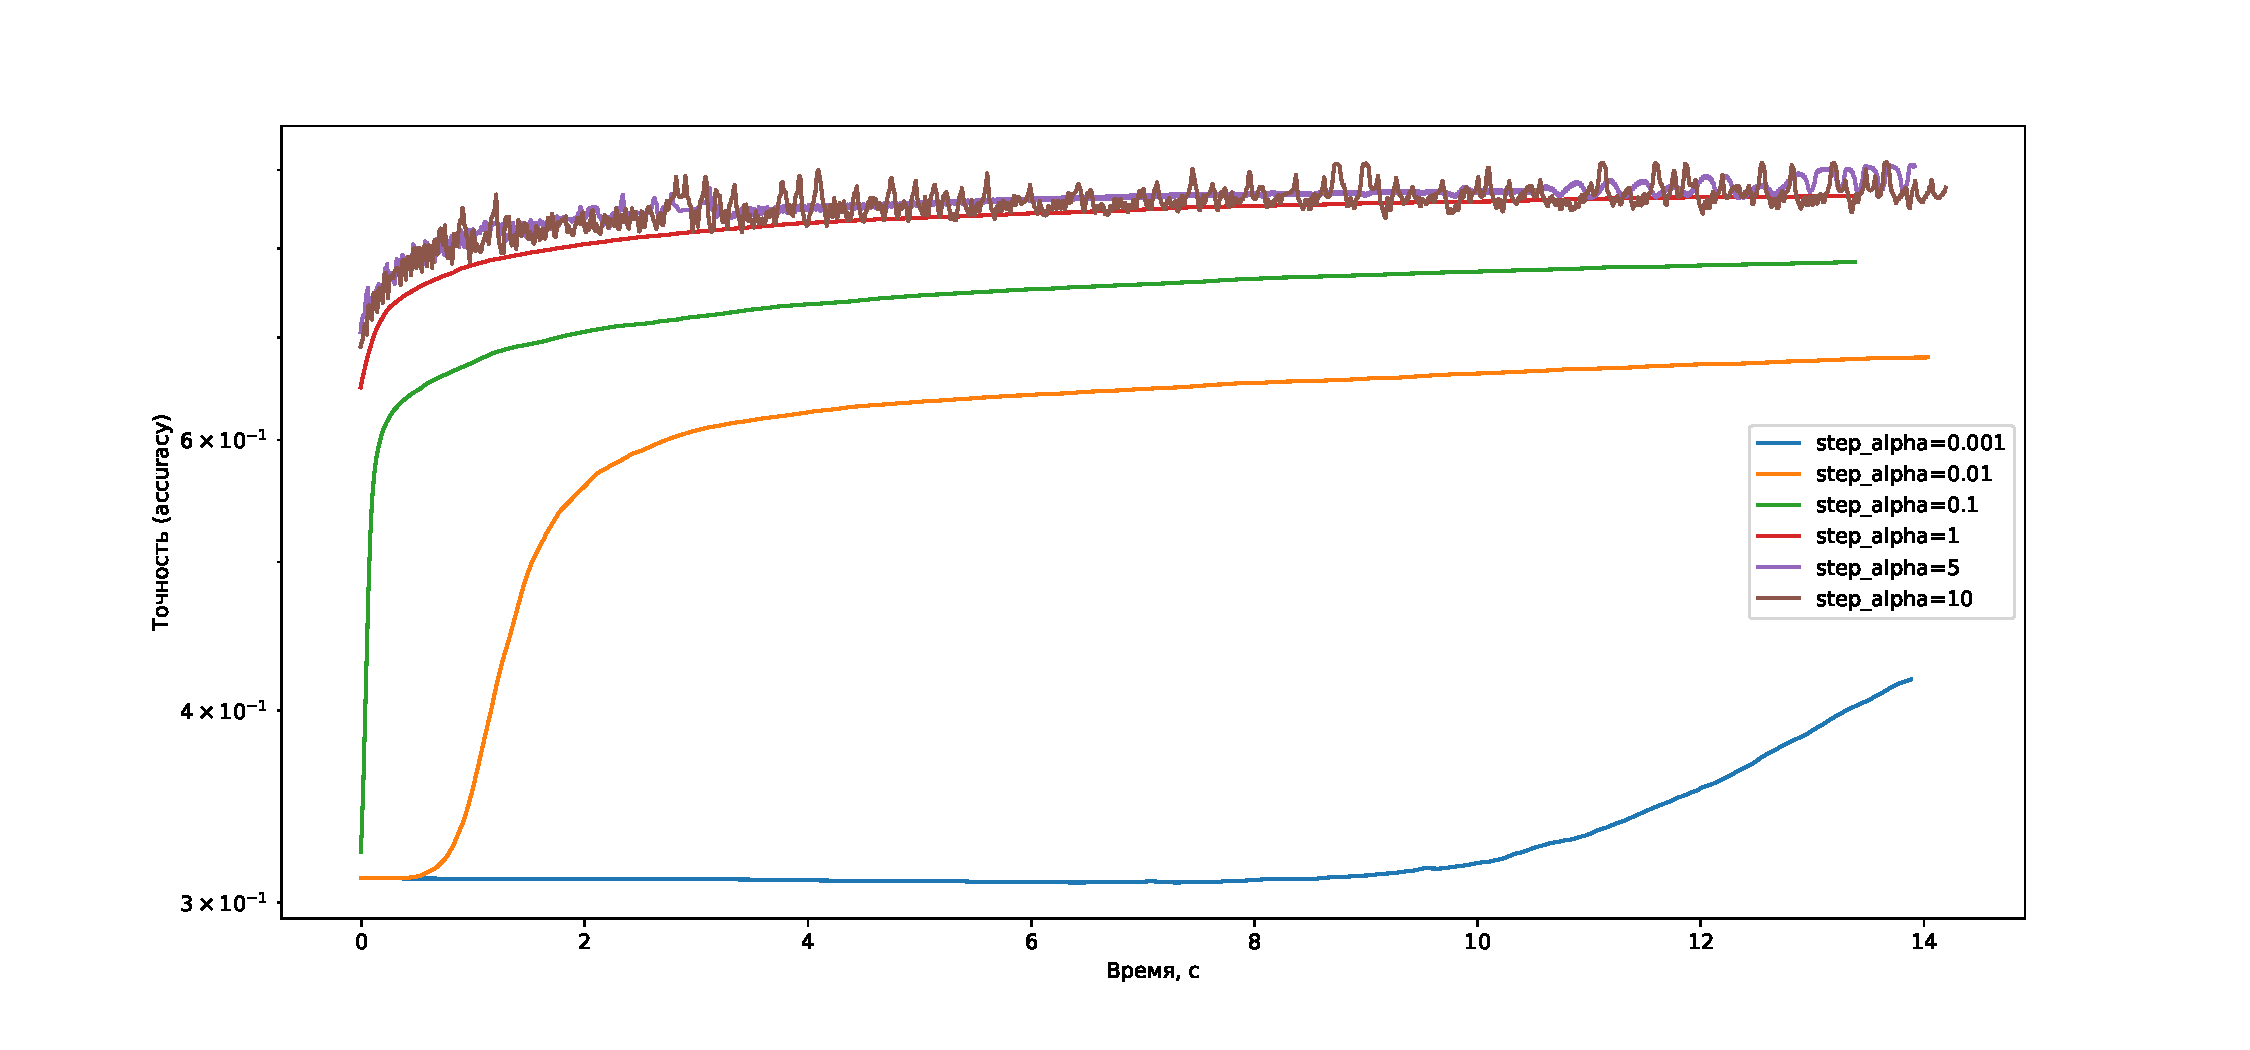
\includegraphics[width=0.5\textwidth, height=0.25\textheight]{../graphs/exp1_accuracy_GD_alpha_time_beta=0,001.pdf}
                    \end{center}
                \end{multicols}
            \end{figure}
            \subsubsection{Параметр размера шага step\_beta}
            Параметр \textbf{step\_beta $(\beta)$} используется в градиентном спуске при обновлении весов в формуле \ref{exp1:weight_upd}.
            Аналогично предыдущему пункту рассмотрим зависимости из \ref{exp:dependencies_sgd} при разных значениях параметра \textbf{step\_beta} и проанализруем соответсвующие графики, представленные на рис. \ref{exp2:sgd_func_time}, \ref{exp2:sgd_acc_time}, \ref{exp2:sgd_func_iter}, \ref{exp2:sgd_acc_iter}.
            
            
            \begin{figure}[H] \label{exp1}
                \begin{multicols}{2}
                    \begin{center}
                        \caption{Зависимость значения функции потерь от реального времени работы градиентного спуска} \label{exp2:sgd_func_time}
                        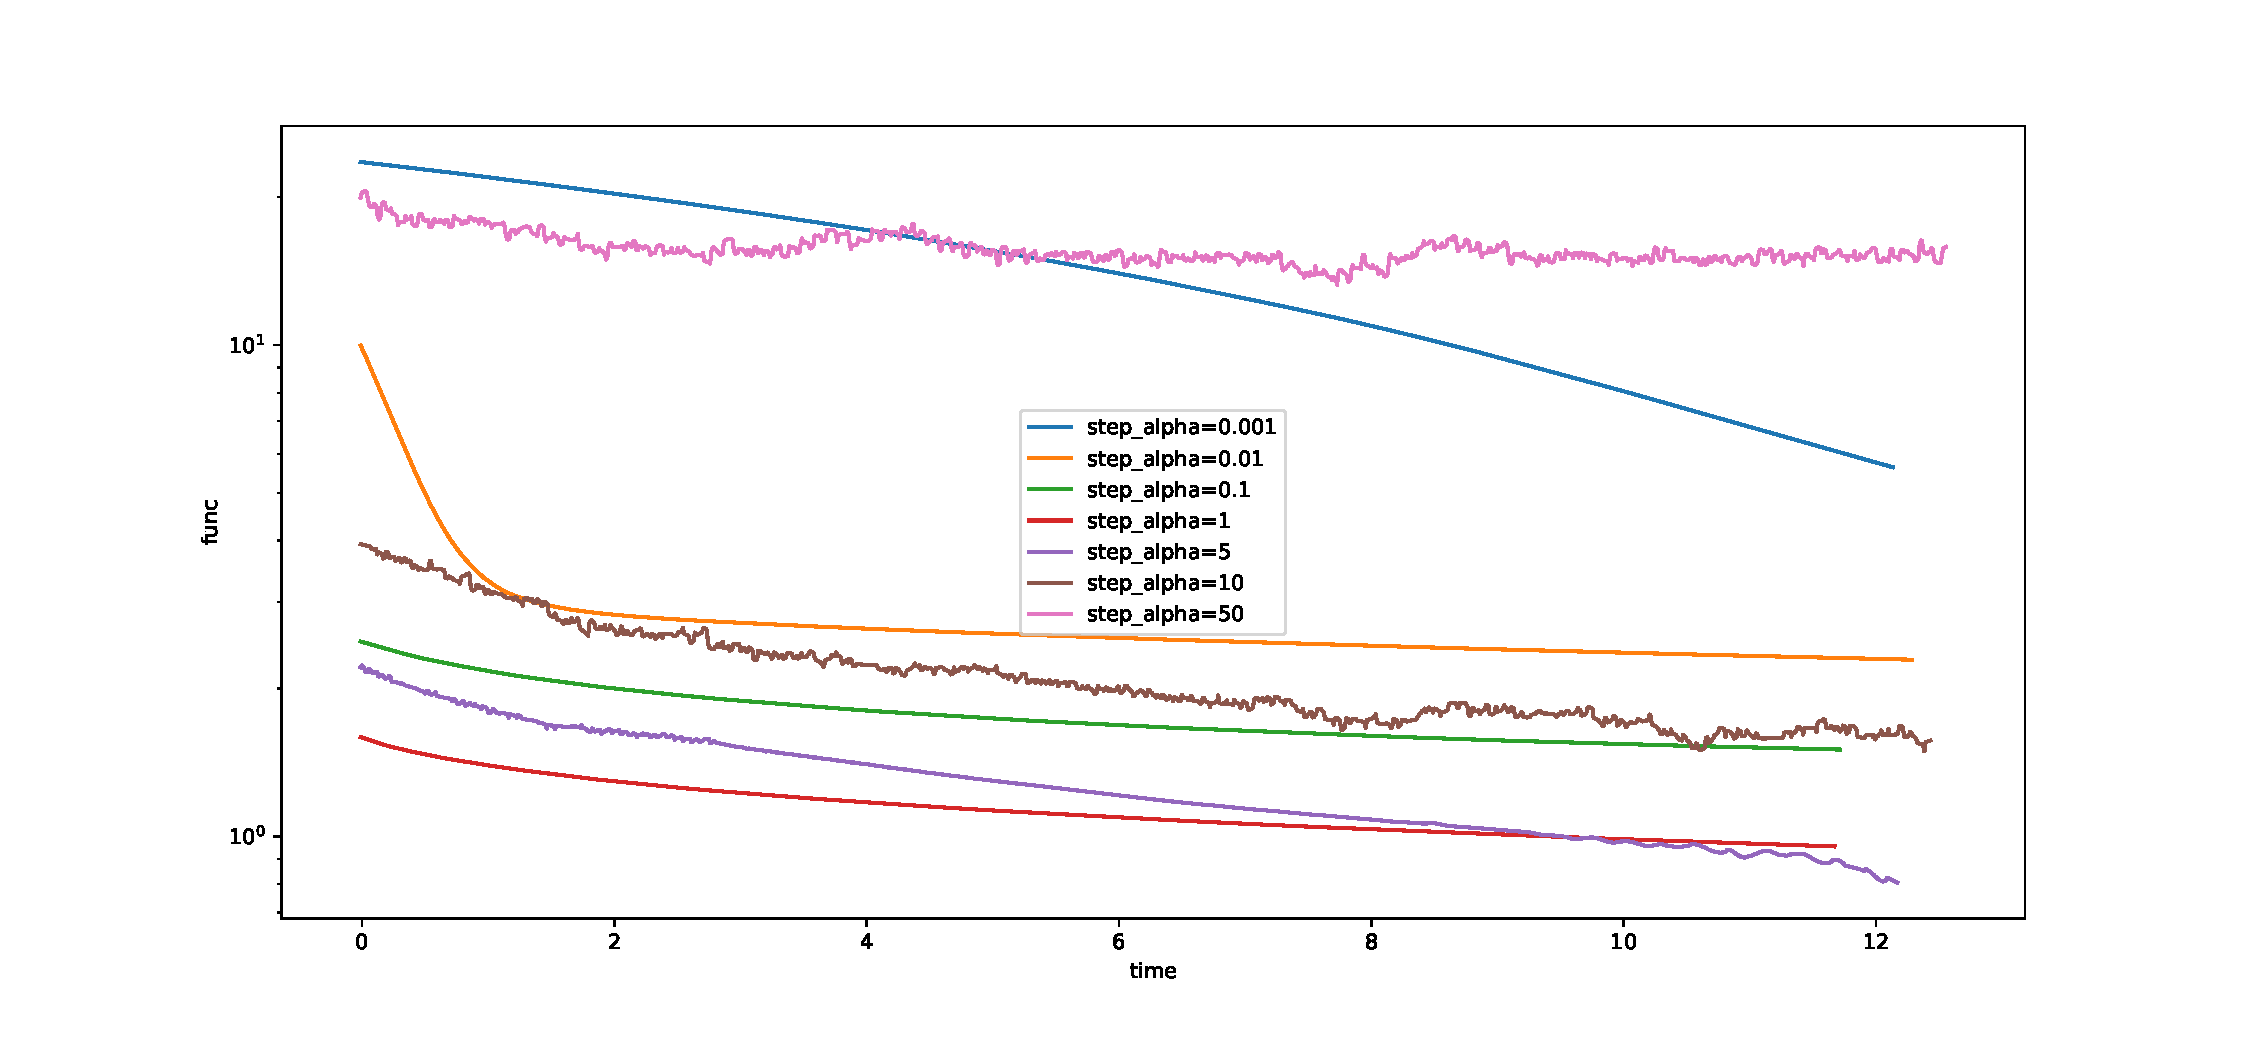
\includegraphics[width=0.5\textwidth, height=0.25\textheight]{../graphs/exp1_func_GD_alpha_time_beta=0,001.pdf}
                        
                        \caption{Зависимость значения точности (accuracy) от реального времени работы градиентного спуска} \label{exp2:sgd_acc_time}
                        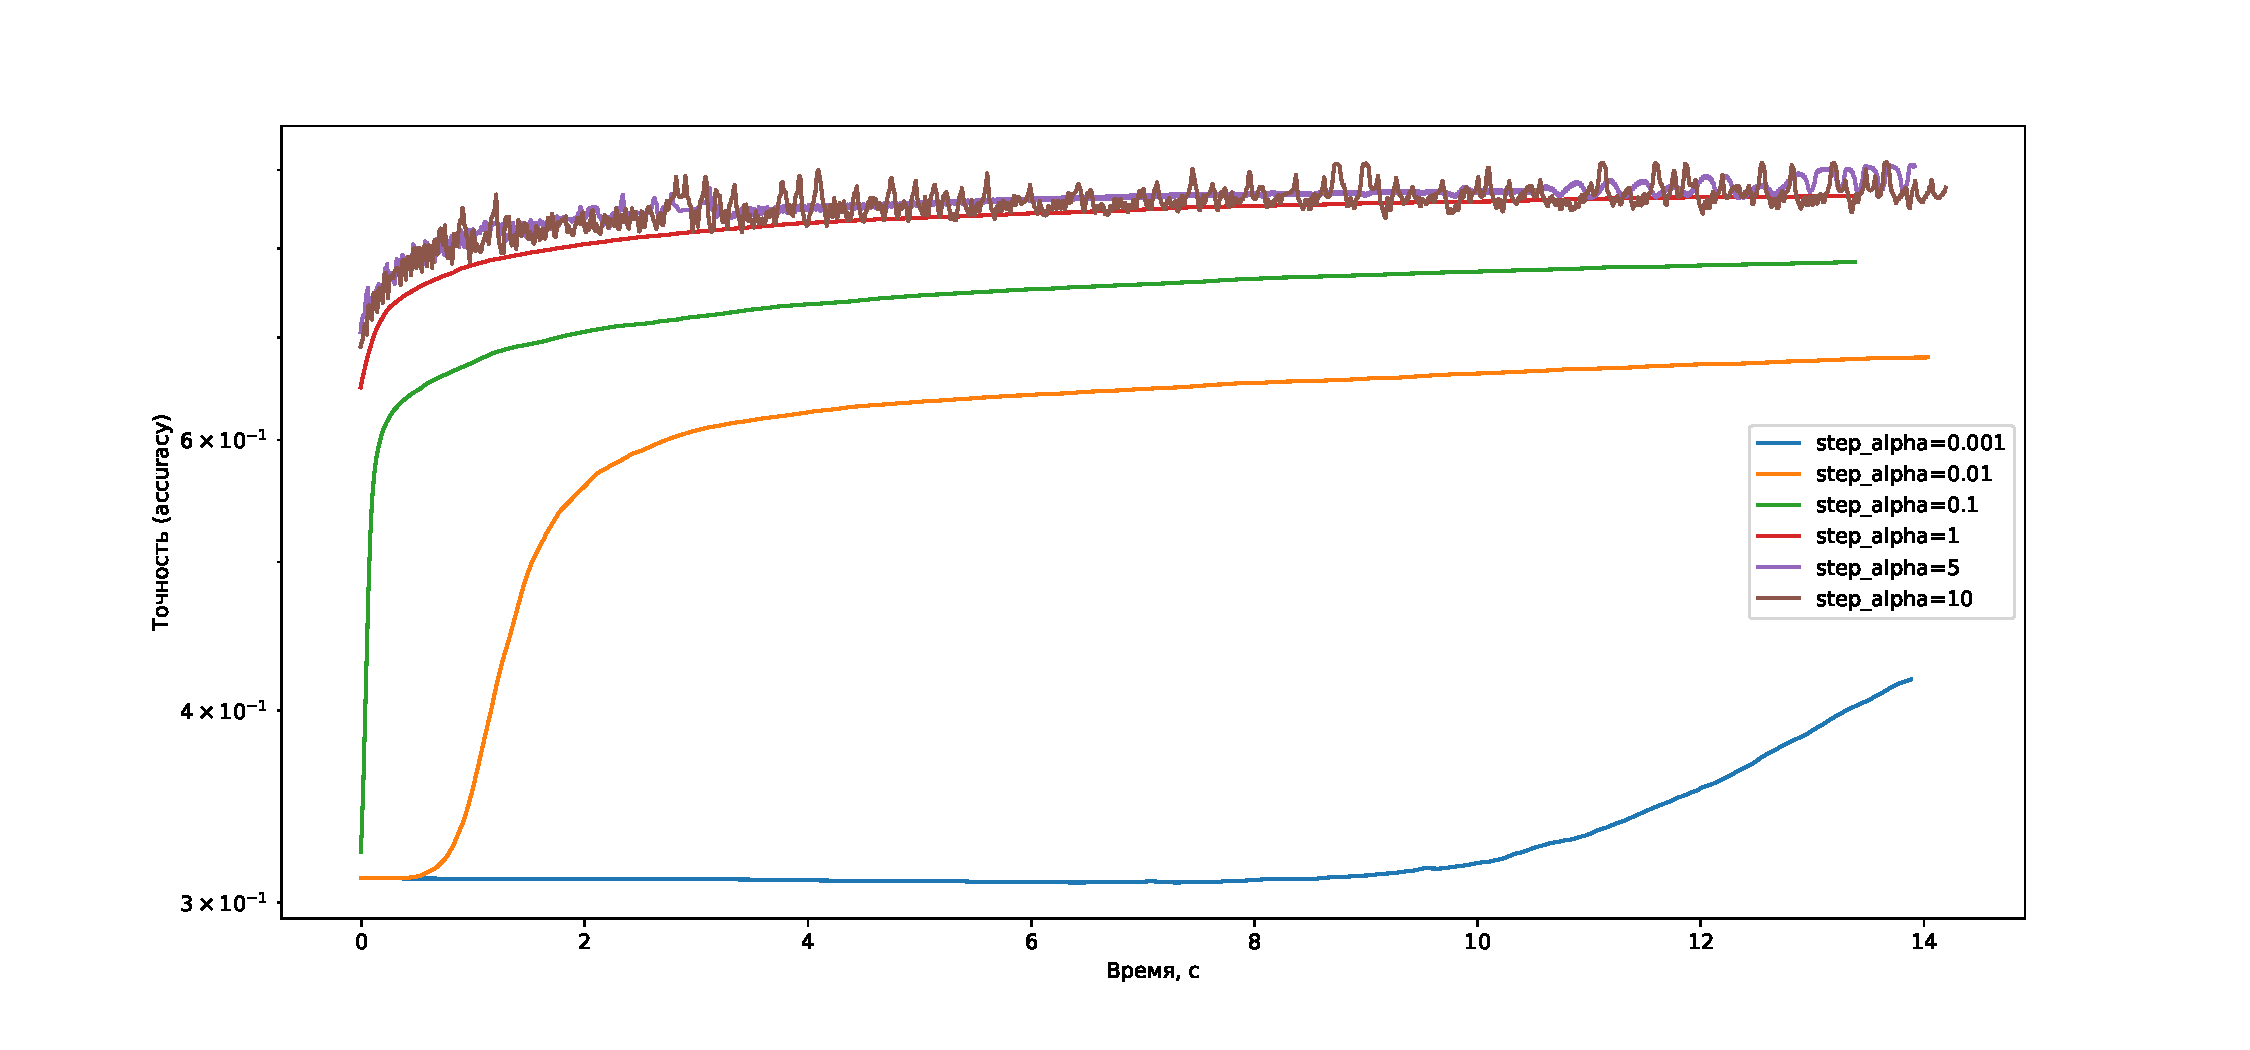
\includegraphics[width=0.5\textwidth, height=0.25\textheight]{../graphs/exp1_accuracy_GD_alpha_time_beta=0,001.pdf}
                        
                        \caption{Зависимость значения функции потерь от эпохи метода градиентного спуска} \label{exp2:sgd_func_iter}
                        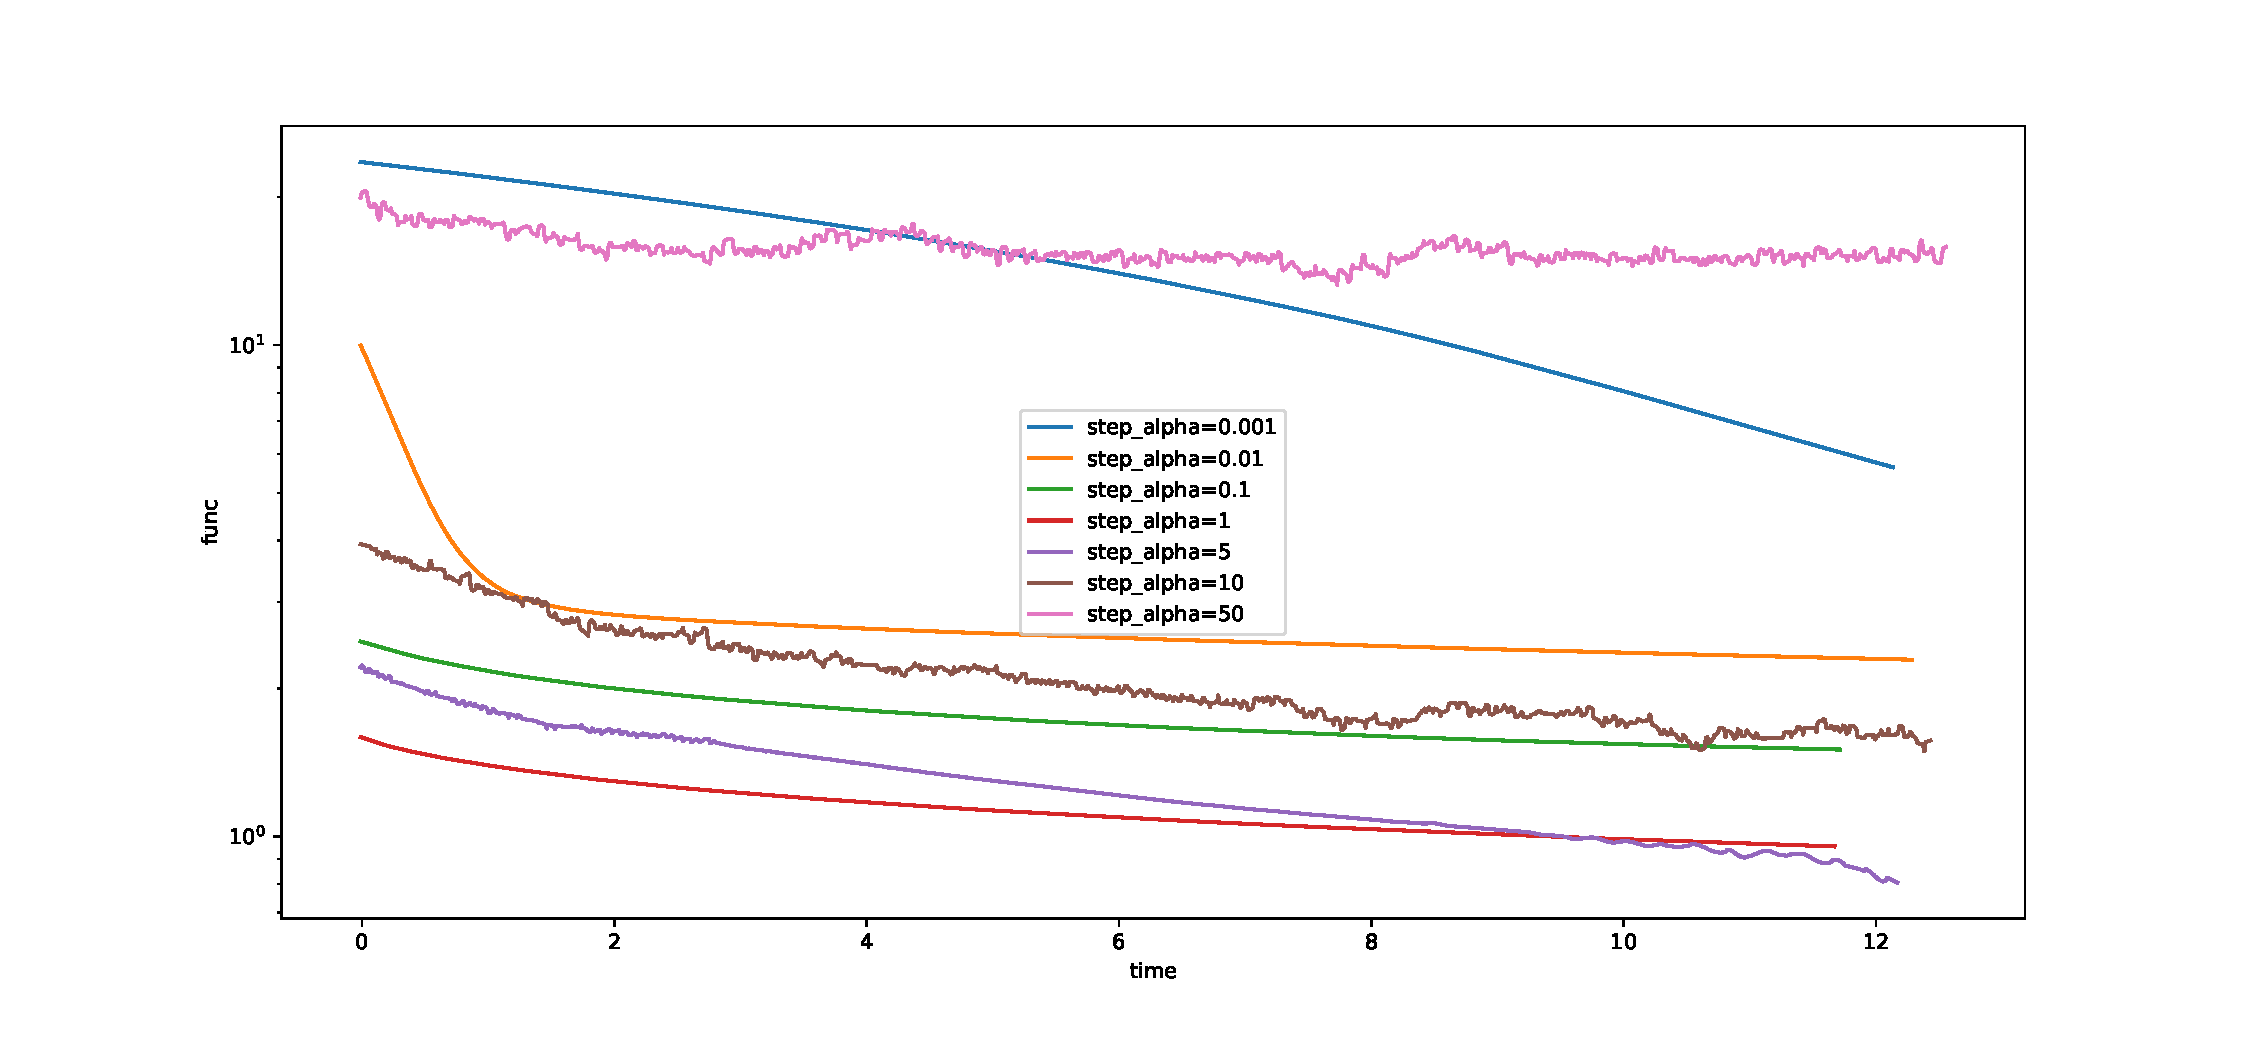
\includegraphics[width=0.5\textwidth, height=0.25\textheight]{../graphs/exp1_func_GD_alpha_time_beta=0,001.pdf}
                        
                        \caption{Зависимость значения точности (accuracy) от эпохи метода градиентного спуска} \label{exp2:sgd_acc_iter}
                        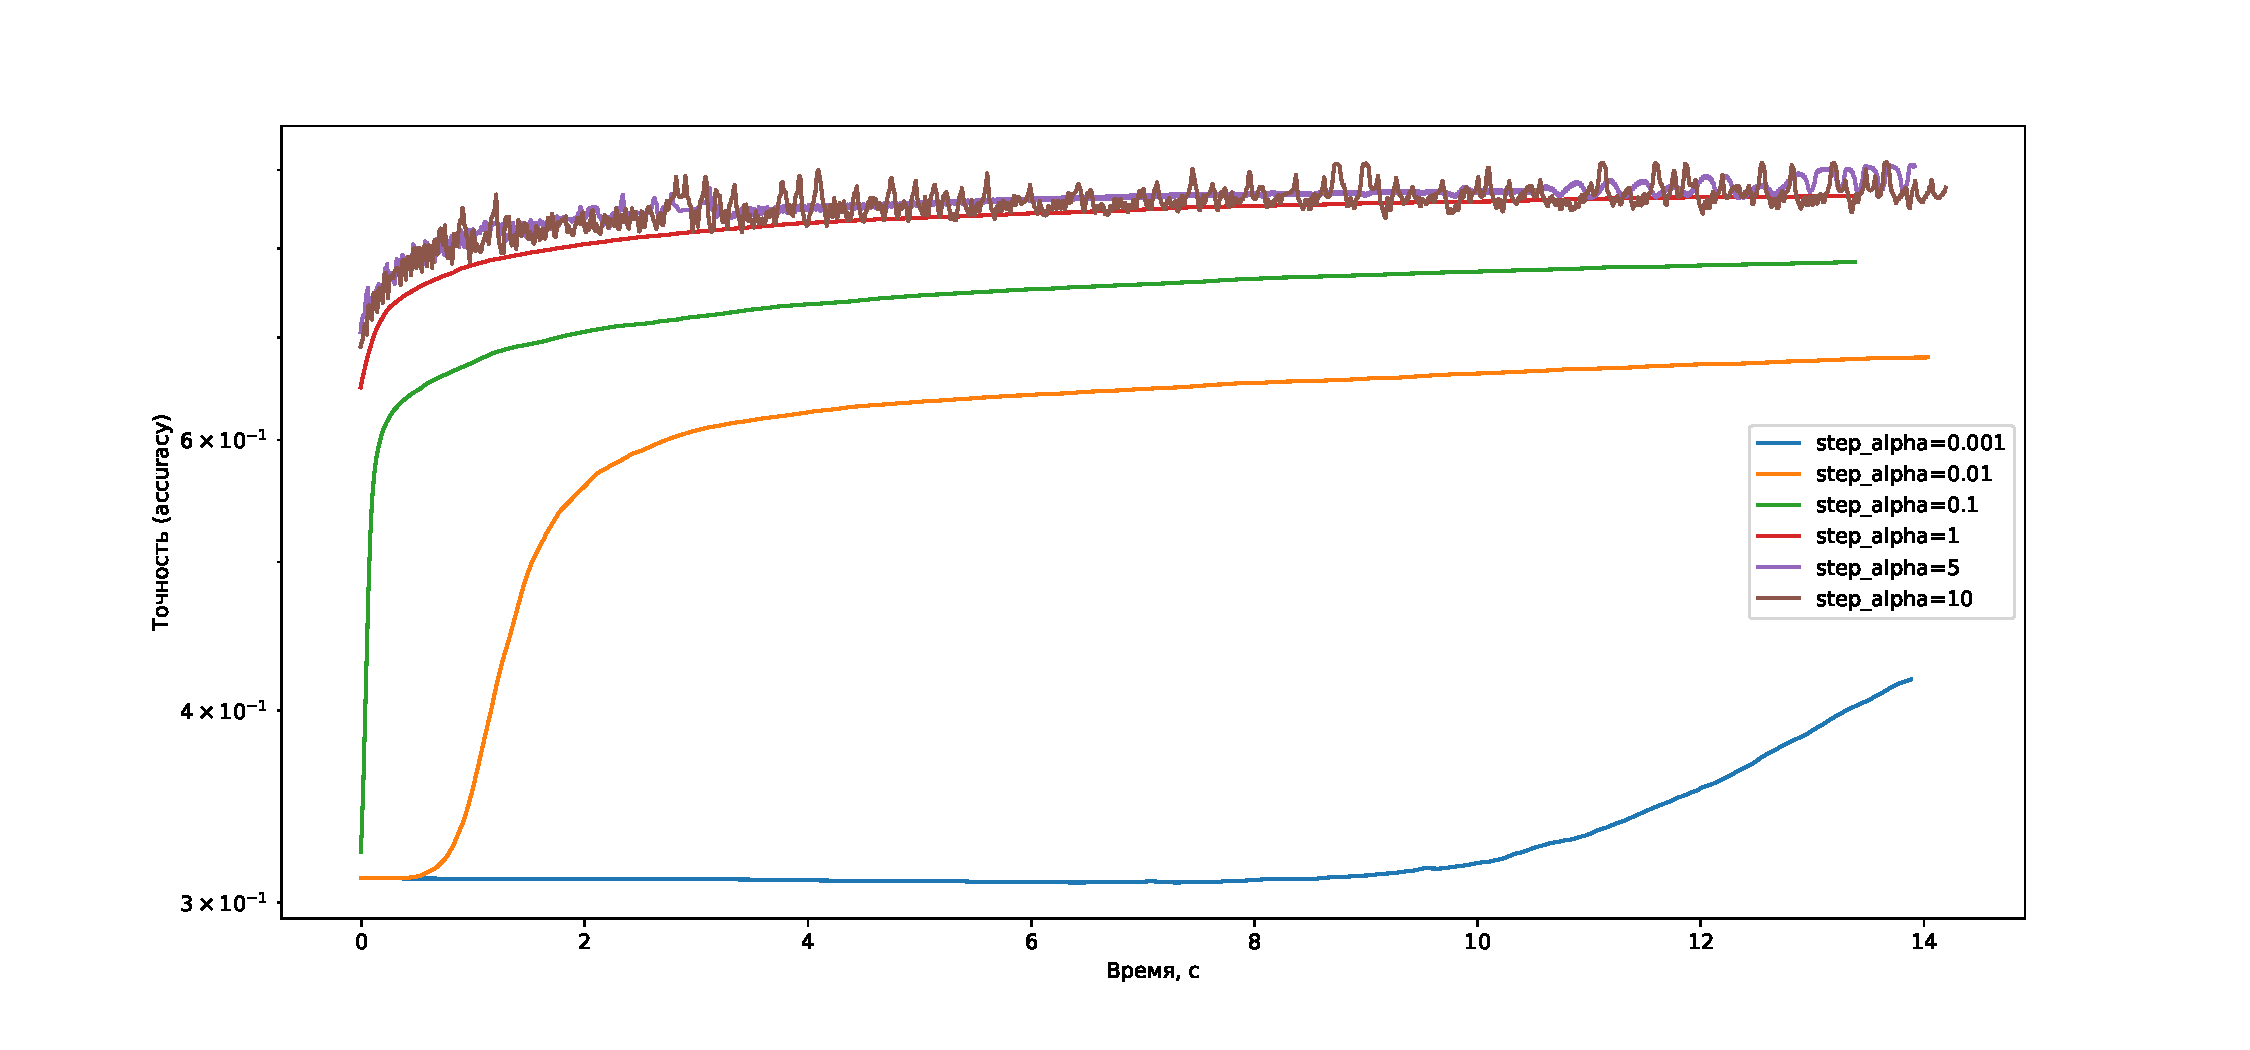
\includegraphics[width=0.5\textwidth, height=0.25\textheight]{../graphs/exp1_accuracy_GD_alpha_time_beta=0,001.pdf}
                    \end{center}
                \end{multicols}
            \end{figure}
            
            \subsubsection{Размер подвыборки batch\_size}
                Размер подвыборки определяет количество элементов тренировочной выборки, которые будут использованы для подсчета градиента.
            
            Соответствующие графики приведены на рис. \ref{exp3:sgd_func_time}, \ref{exp3:sgd_acc_time}, \ref{exp3:sgd_func_iter}, \ref{exp3:sgd_acc_iter}.
            \begin{figure}[H] \label{exp1}
                \begin{multicols}{2}
                    \begin{center}
                        \caption{Зависимость значения функции потерь от реального времени работы градиентного спуска} \label{exp3:sgd_func_time}
                        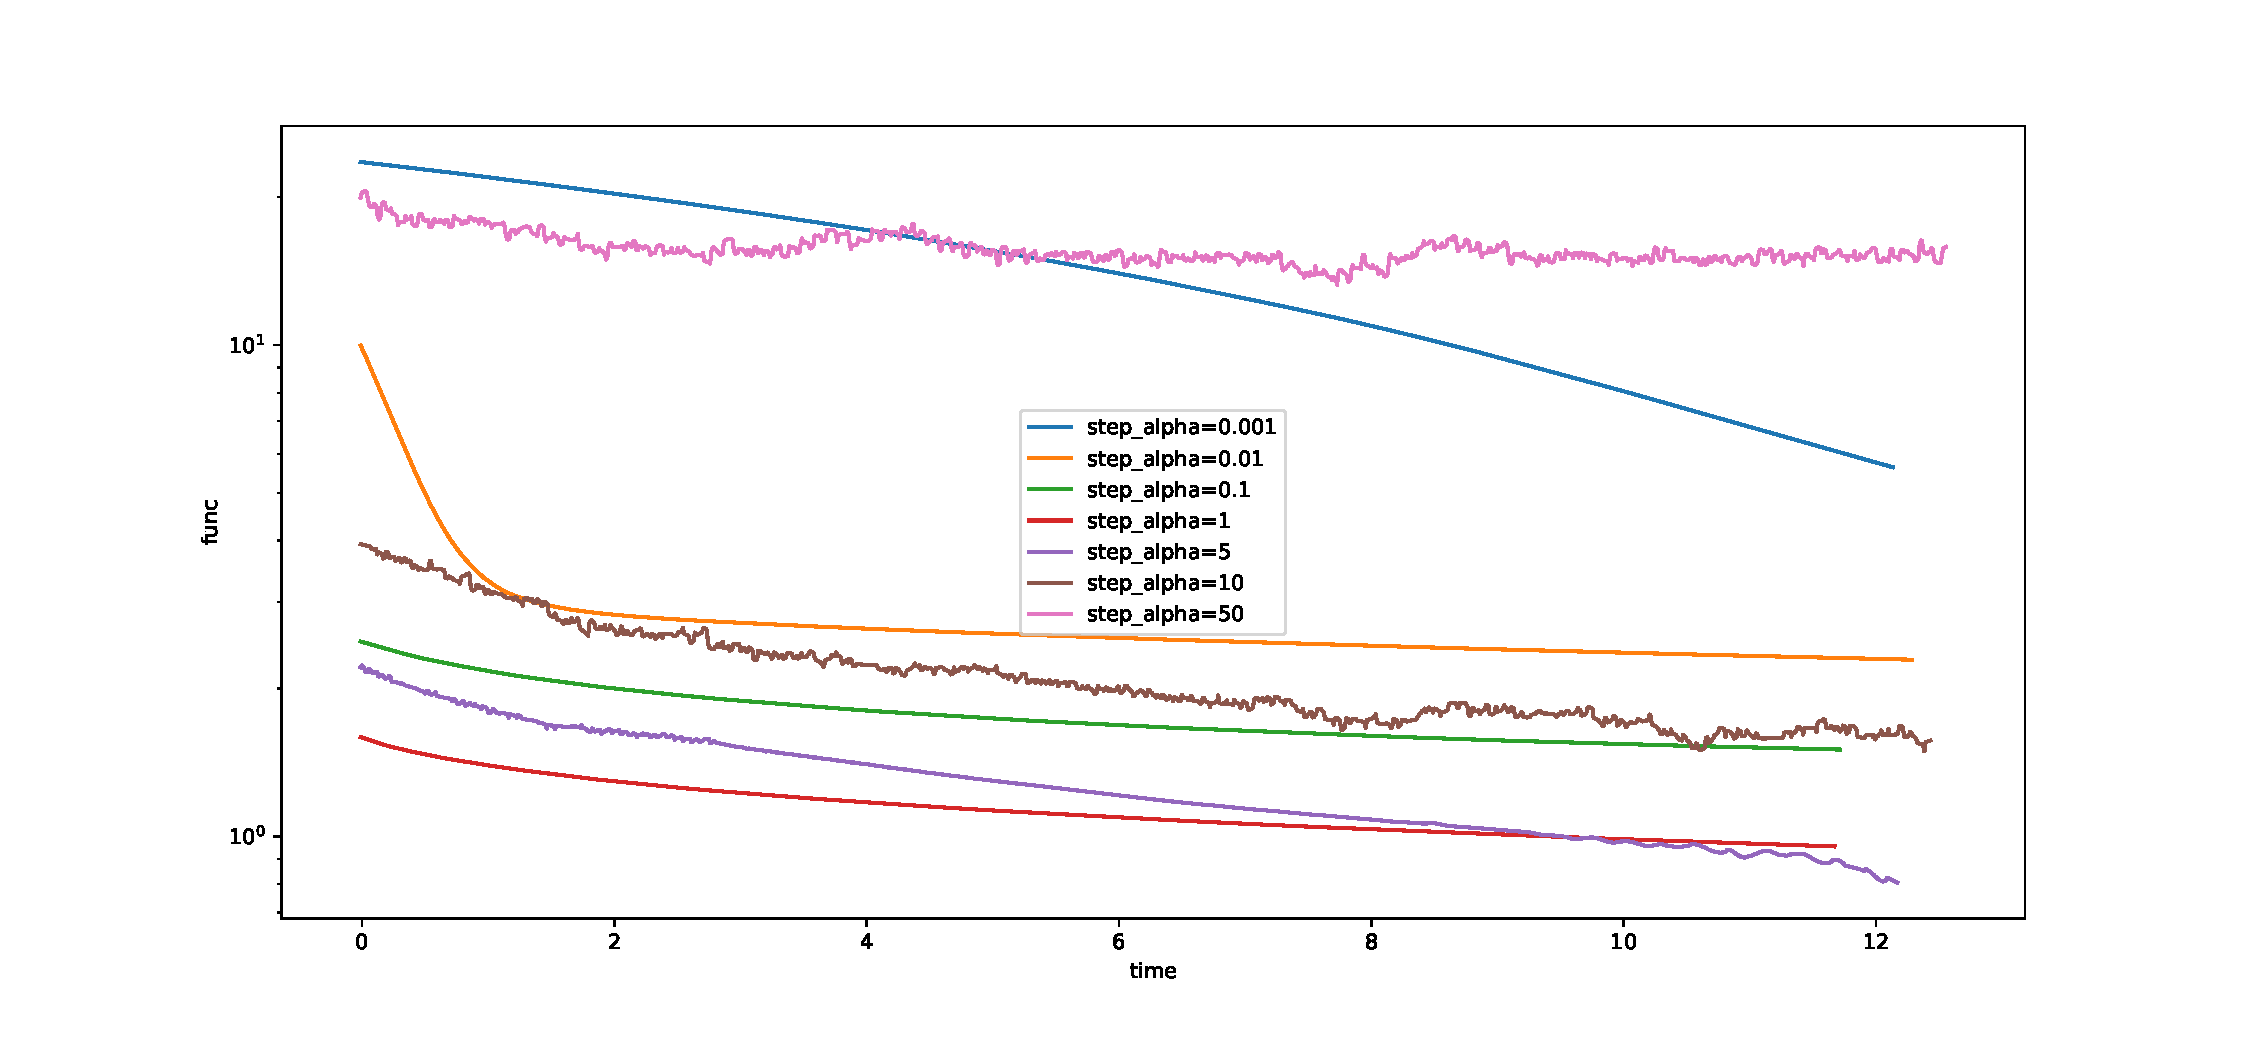
\includegraphics[width=0.5\textwidth, height=0.25\textheight]{../graphs/exp1_func_GD_alpha_time_beta=0,001.pdf}
                        
                        \caption{Зависимость значения точности (accuracy) от реального времени работы градиентного спуска} \label{exp3:sgd_acc_time}
                        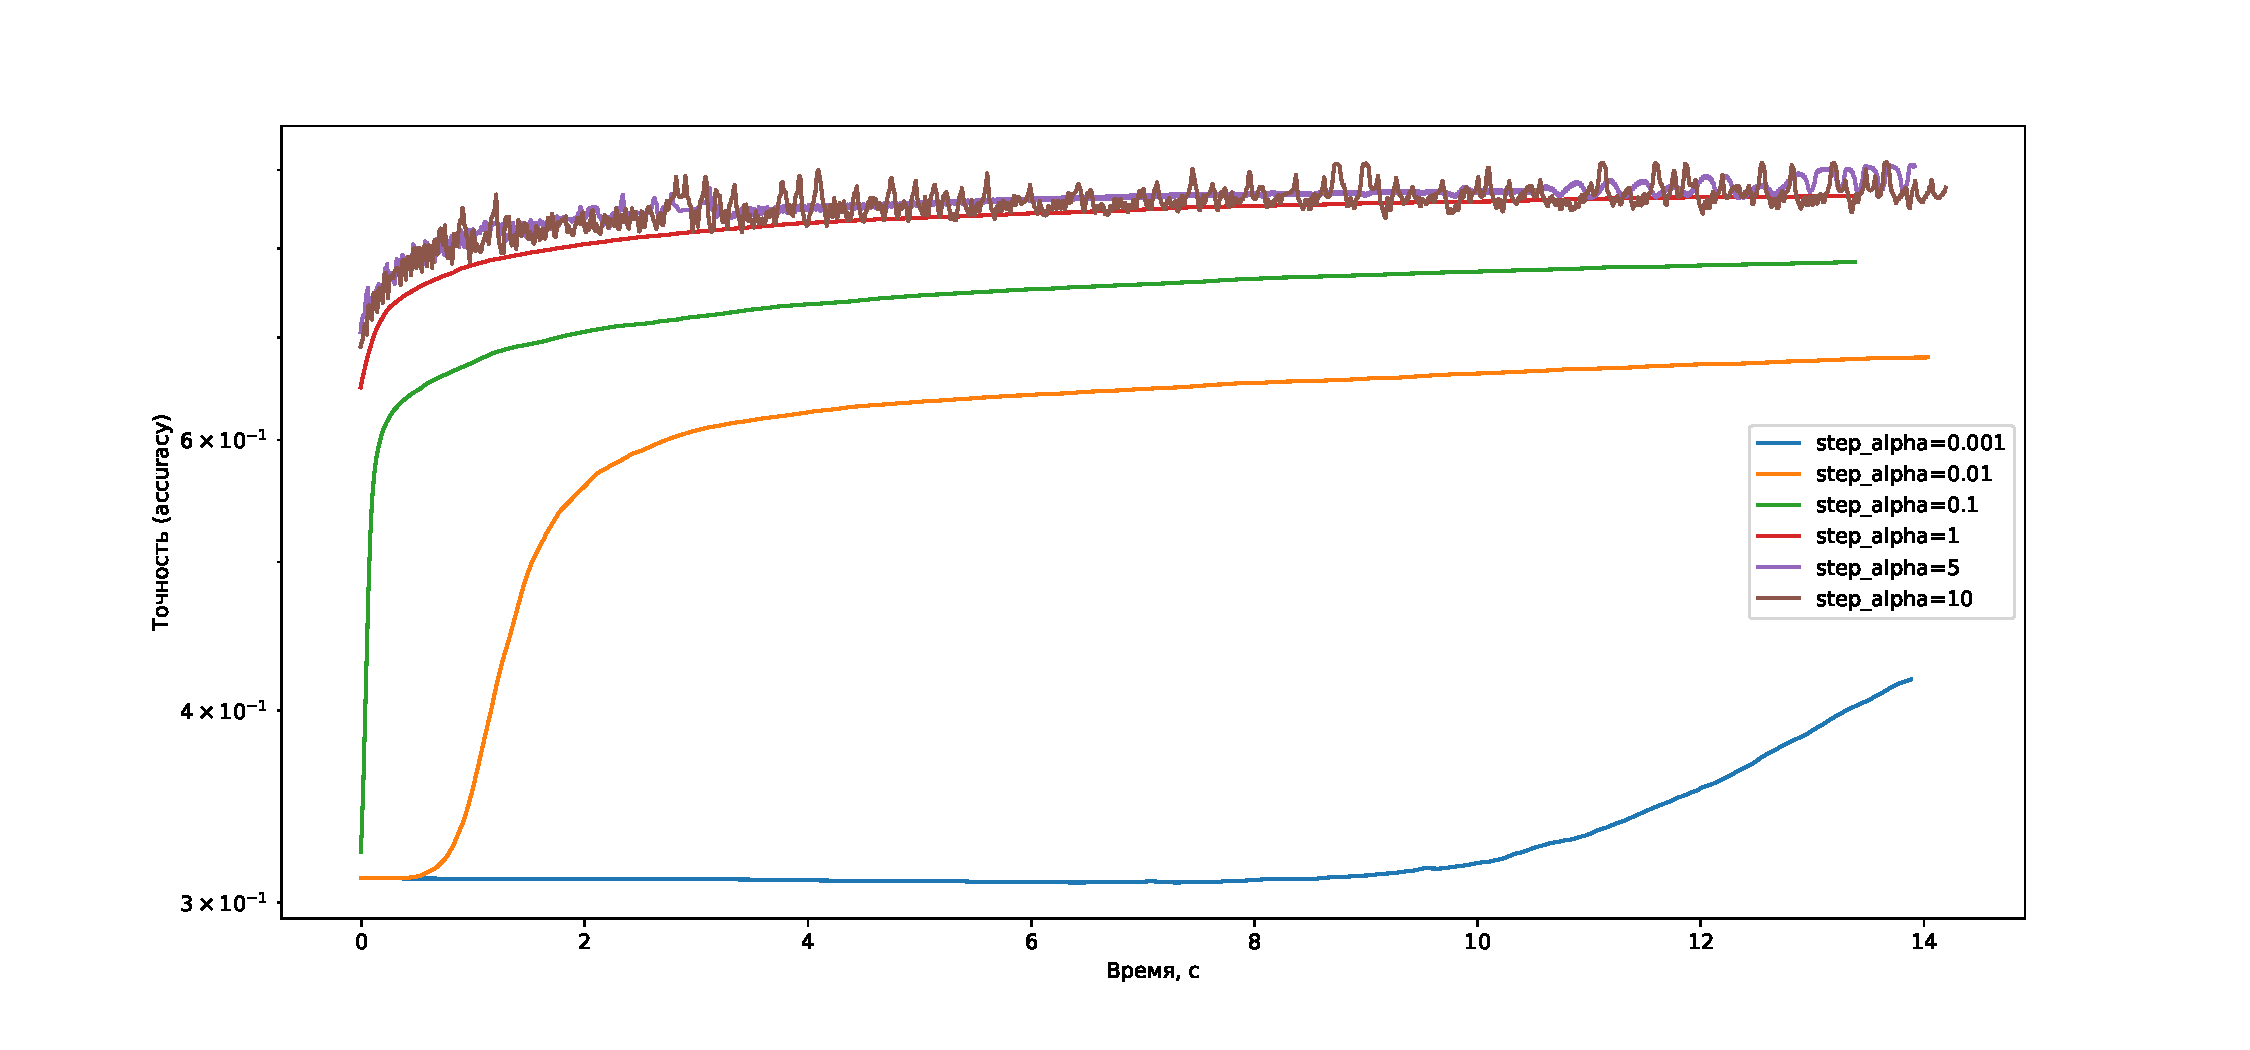
\includegraphics[width=0.5\textwidth, height=0.25\textheight]{../graphs/exp1_accuracy_GD_alpha_time_beta=0,001.pdf}
                        
                        \caption{Зависимость значения функции потерь от эпохи метода градиентного спуска} \label{exp3:sgd_func_iter}
                        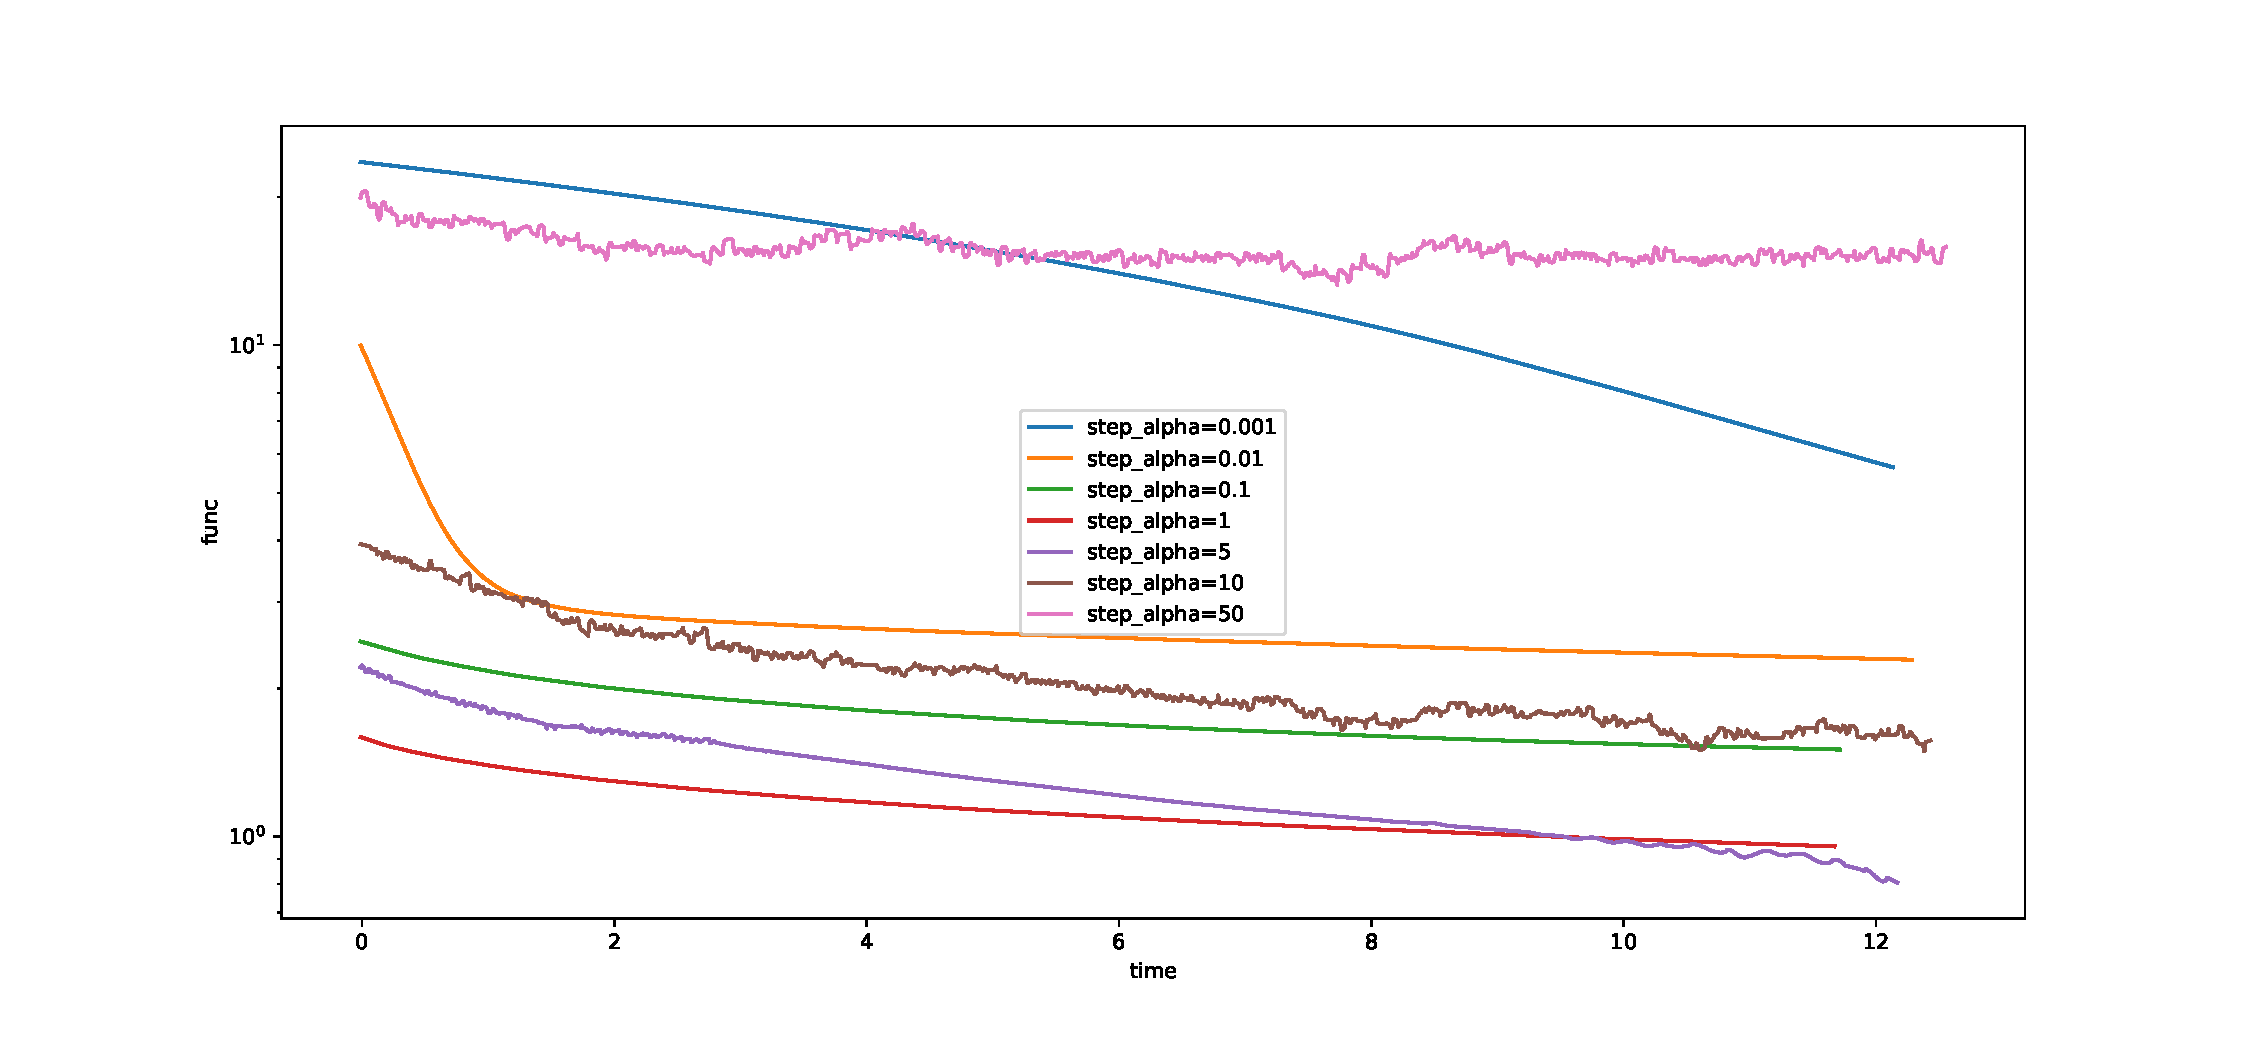
\includegraphics[width=0.5\textwidth, height=0.25\textheight]{../graphs/exp1_func_GD_alpha_time_beta=0,001.pdf}
                        
                        \caption{Зависимость значения точности (accuracy) от эпохи метода градиентного спуска} \label{exp3:sgd_acc_iter}
                        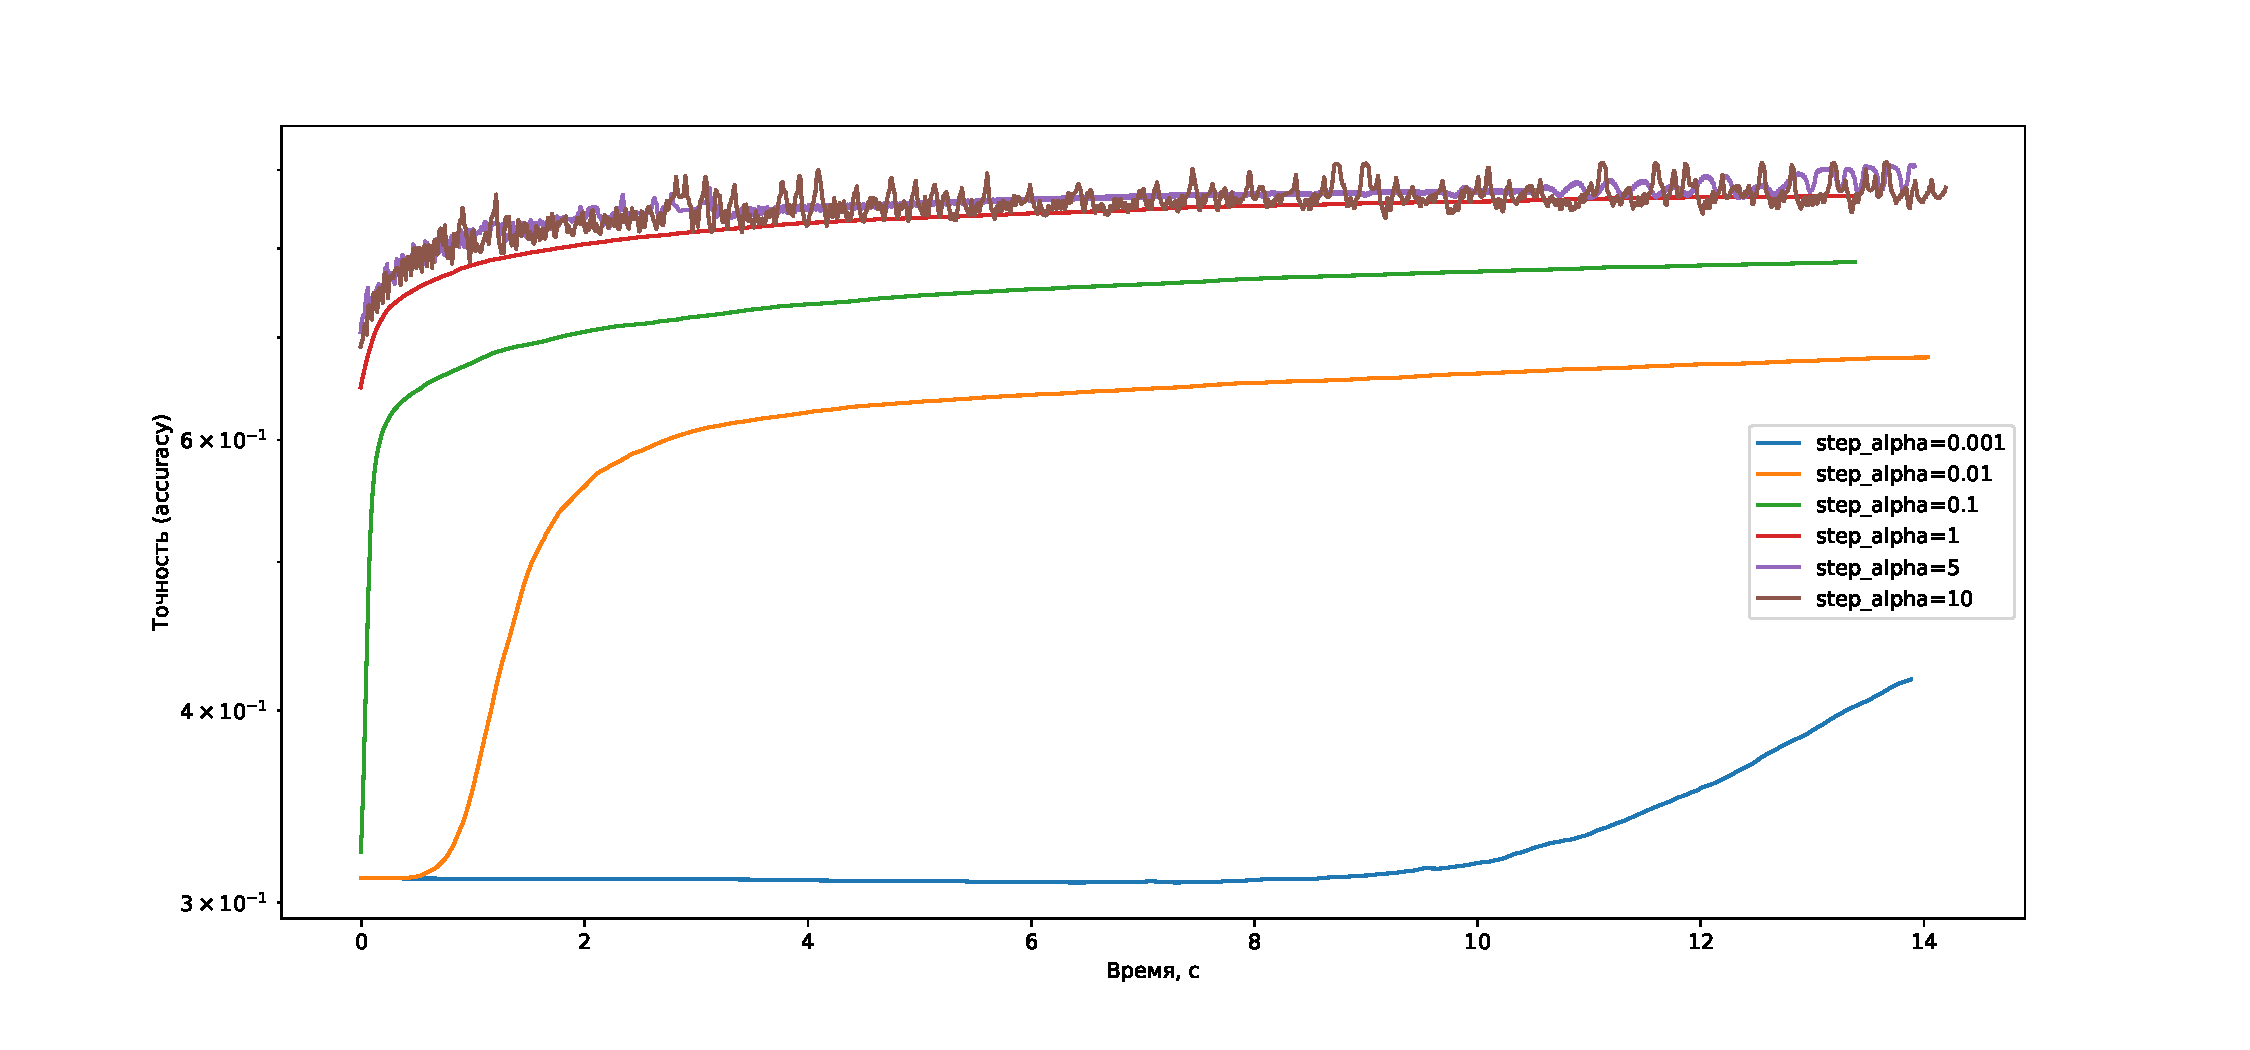
\includegraphics[width=0.5\textwidth, height=0.25\textheight]{../graphs/exp1_accuracy_GD_alpha_time_beta=0,001.pdf}
                    \end{center}
                \end{multicols}
            \end{figure}
            
            \subsubsection{Начальное приближение $w_0$}
            Начальное приближение нужно для инициализации весов модели. В данной работе были рассмотрены следующие варианты задания $w_0$:
            \begin{itemize}
                \item нулевой вектор
                \item вектор с координатами из $U(0, 1)$
                \item вектор с координатами из $U(100, 500)$
                \item вектор с координатами из $U(1000, 5000)$
                \item вектор с координатами из $U(10000, 50000)$
                \item вектор с координатами из $N(0, 1)$
                \item вектор с координатами из $N(0.5, 0.5)$
            \end{itemize}
            Графики зависимостей \ref{exp:dependencies_sgd} представлены на рис. \ref{exp4:sgd_func_time}, \ref{exp4:sgd_acc_time}, \ref{exp4:sgd_func_iter}, \ref{exp4:sgd_acc_iter}.
            \begin{figure}[H] \label{exp1}
                \begin{multicols}{2}
                    \begin{center}
                        \caption{Зависимость значения функции потерь от реального времени работы градиентного спуска} \label{exp4:sgd_func_time}
                        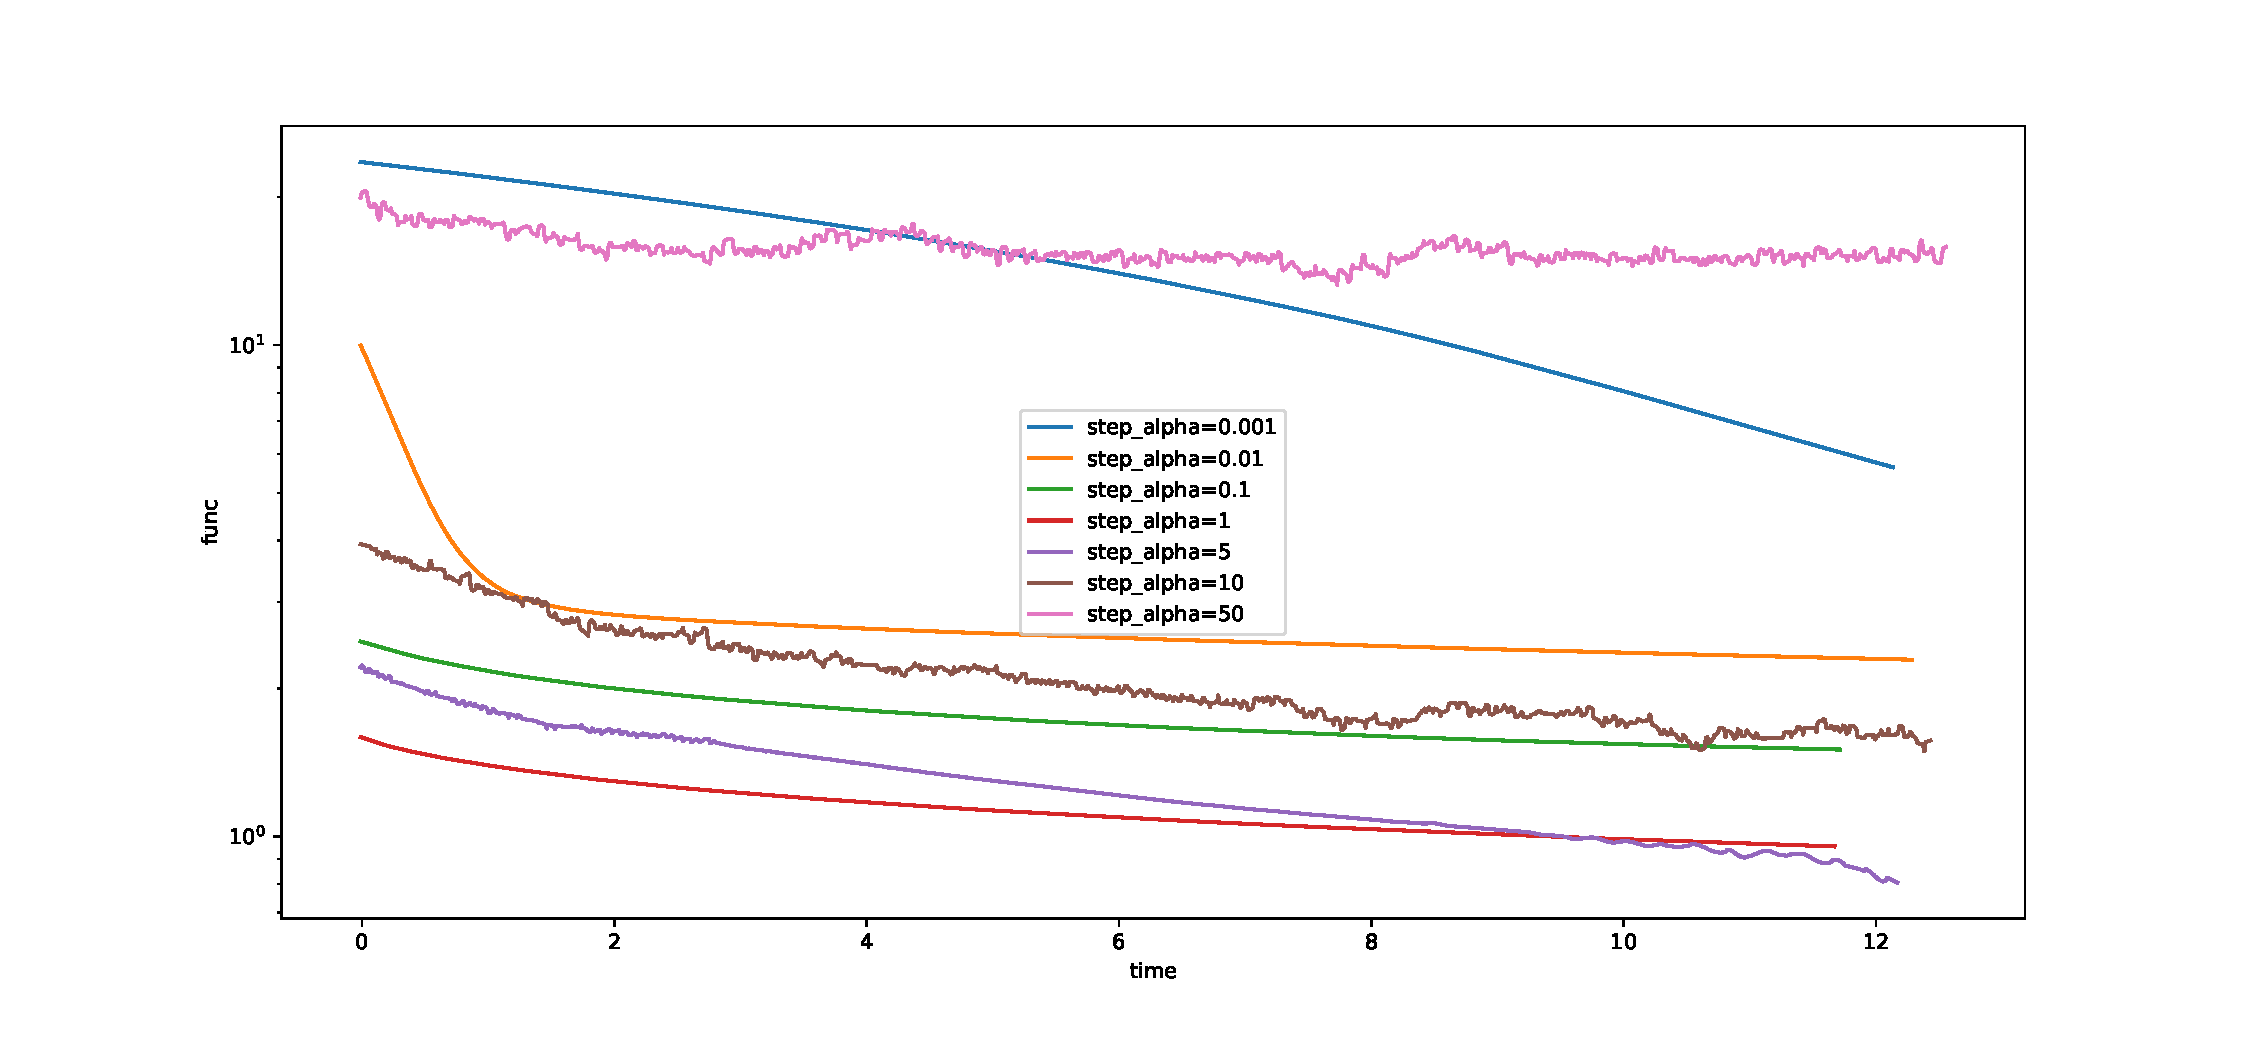
\includegraphics[width=0.5\textwidth, height=0.25\textheight]{../graphs/exp1_func_GD_alpha_time_beta=0,001.pdf}
                        
                        \caption{Зависимость значения точности (accuracy) от реального времени работы градиентного спуска} \label{exp4:sgd_acc_time}
                        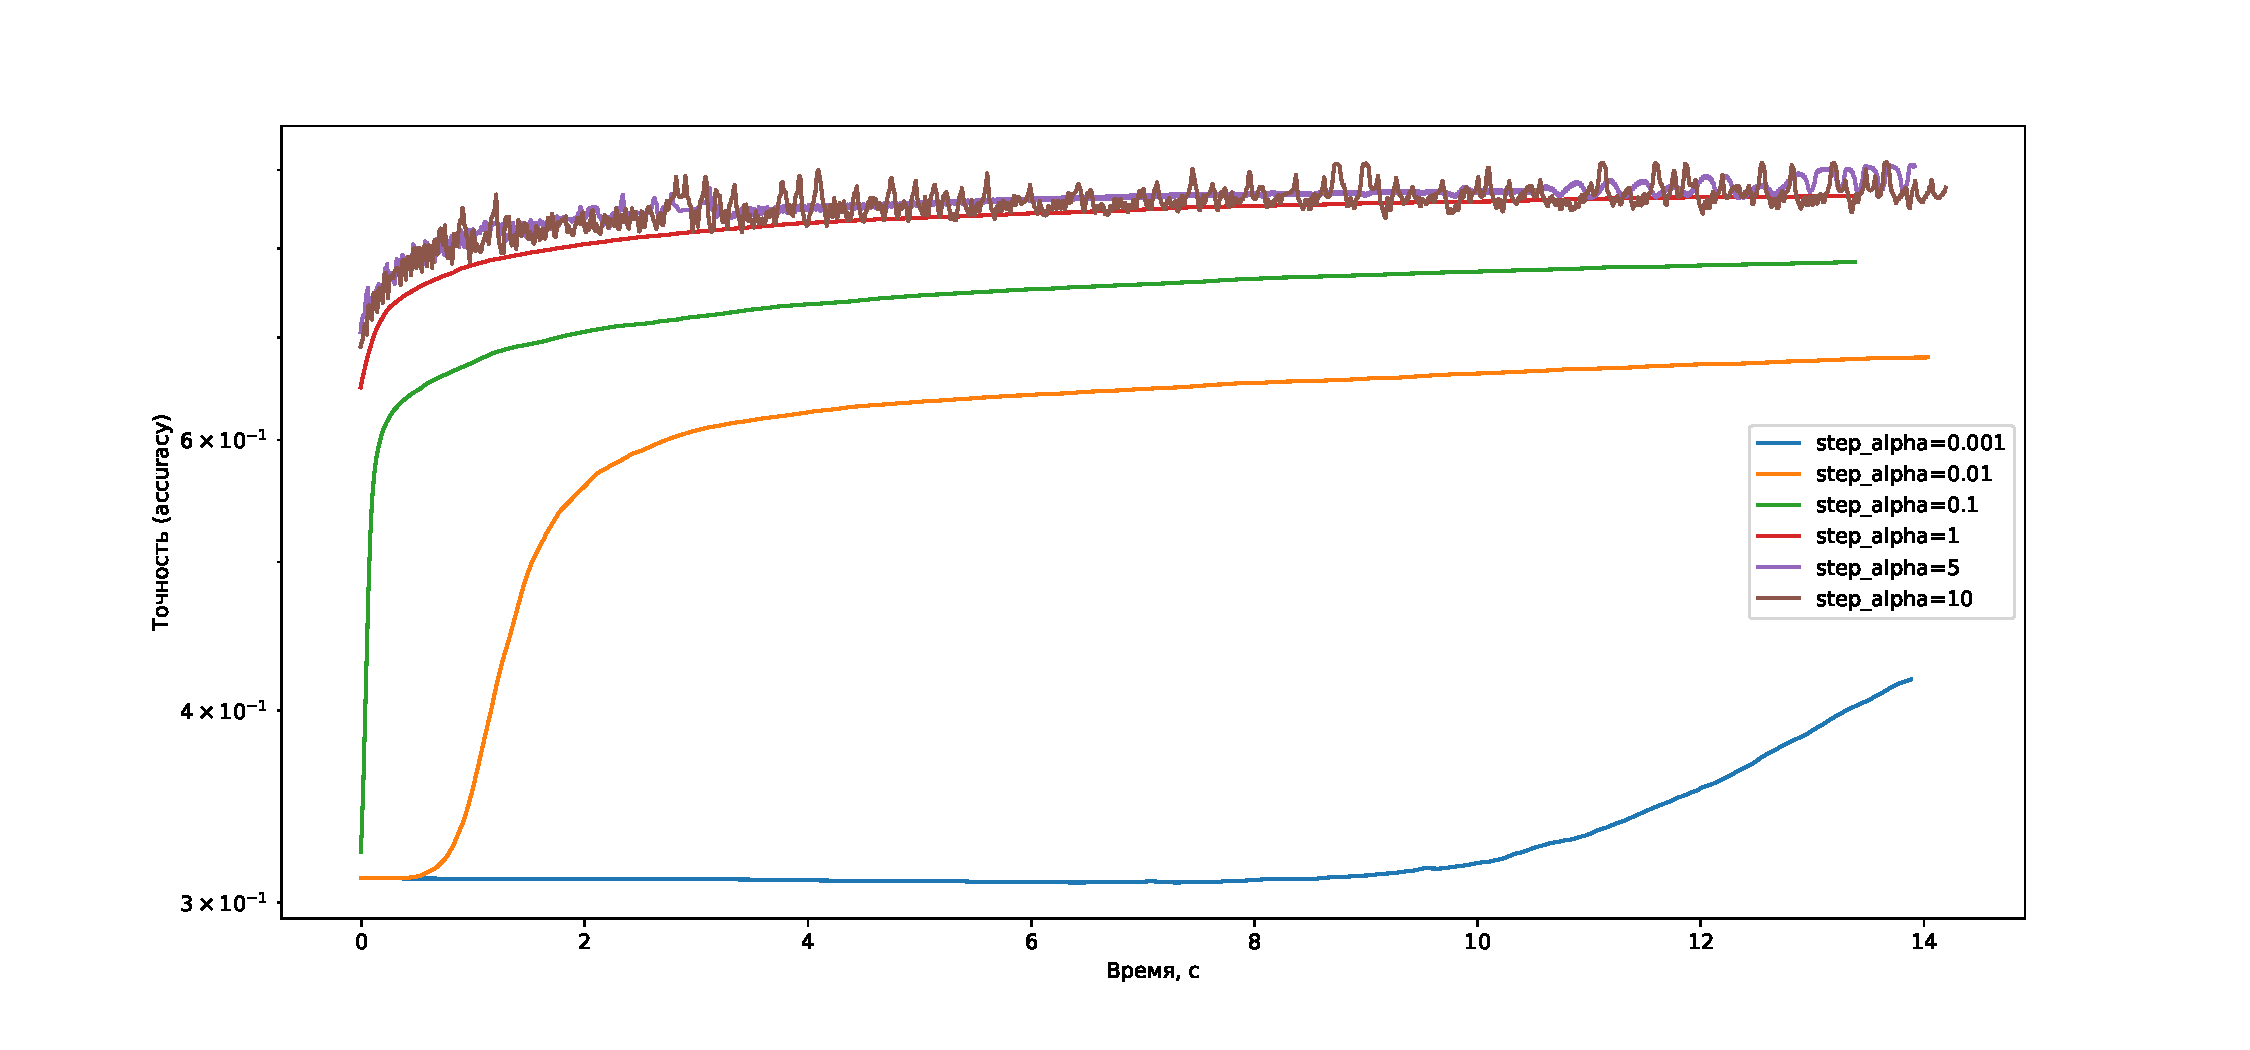
\includegraphics[width=0.5\textwidth, height=0.25\textheight]{../graphs/exp1_accuracy_GD_alpha_time_beta=0,001.pdf}
                        
                        \caption{Зависимость значения функции потерь от эпохи метода градиентного спуска} \label{exp4:sgd_func_iter}
                        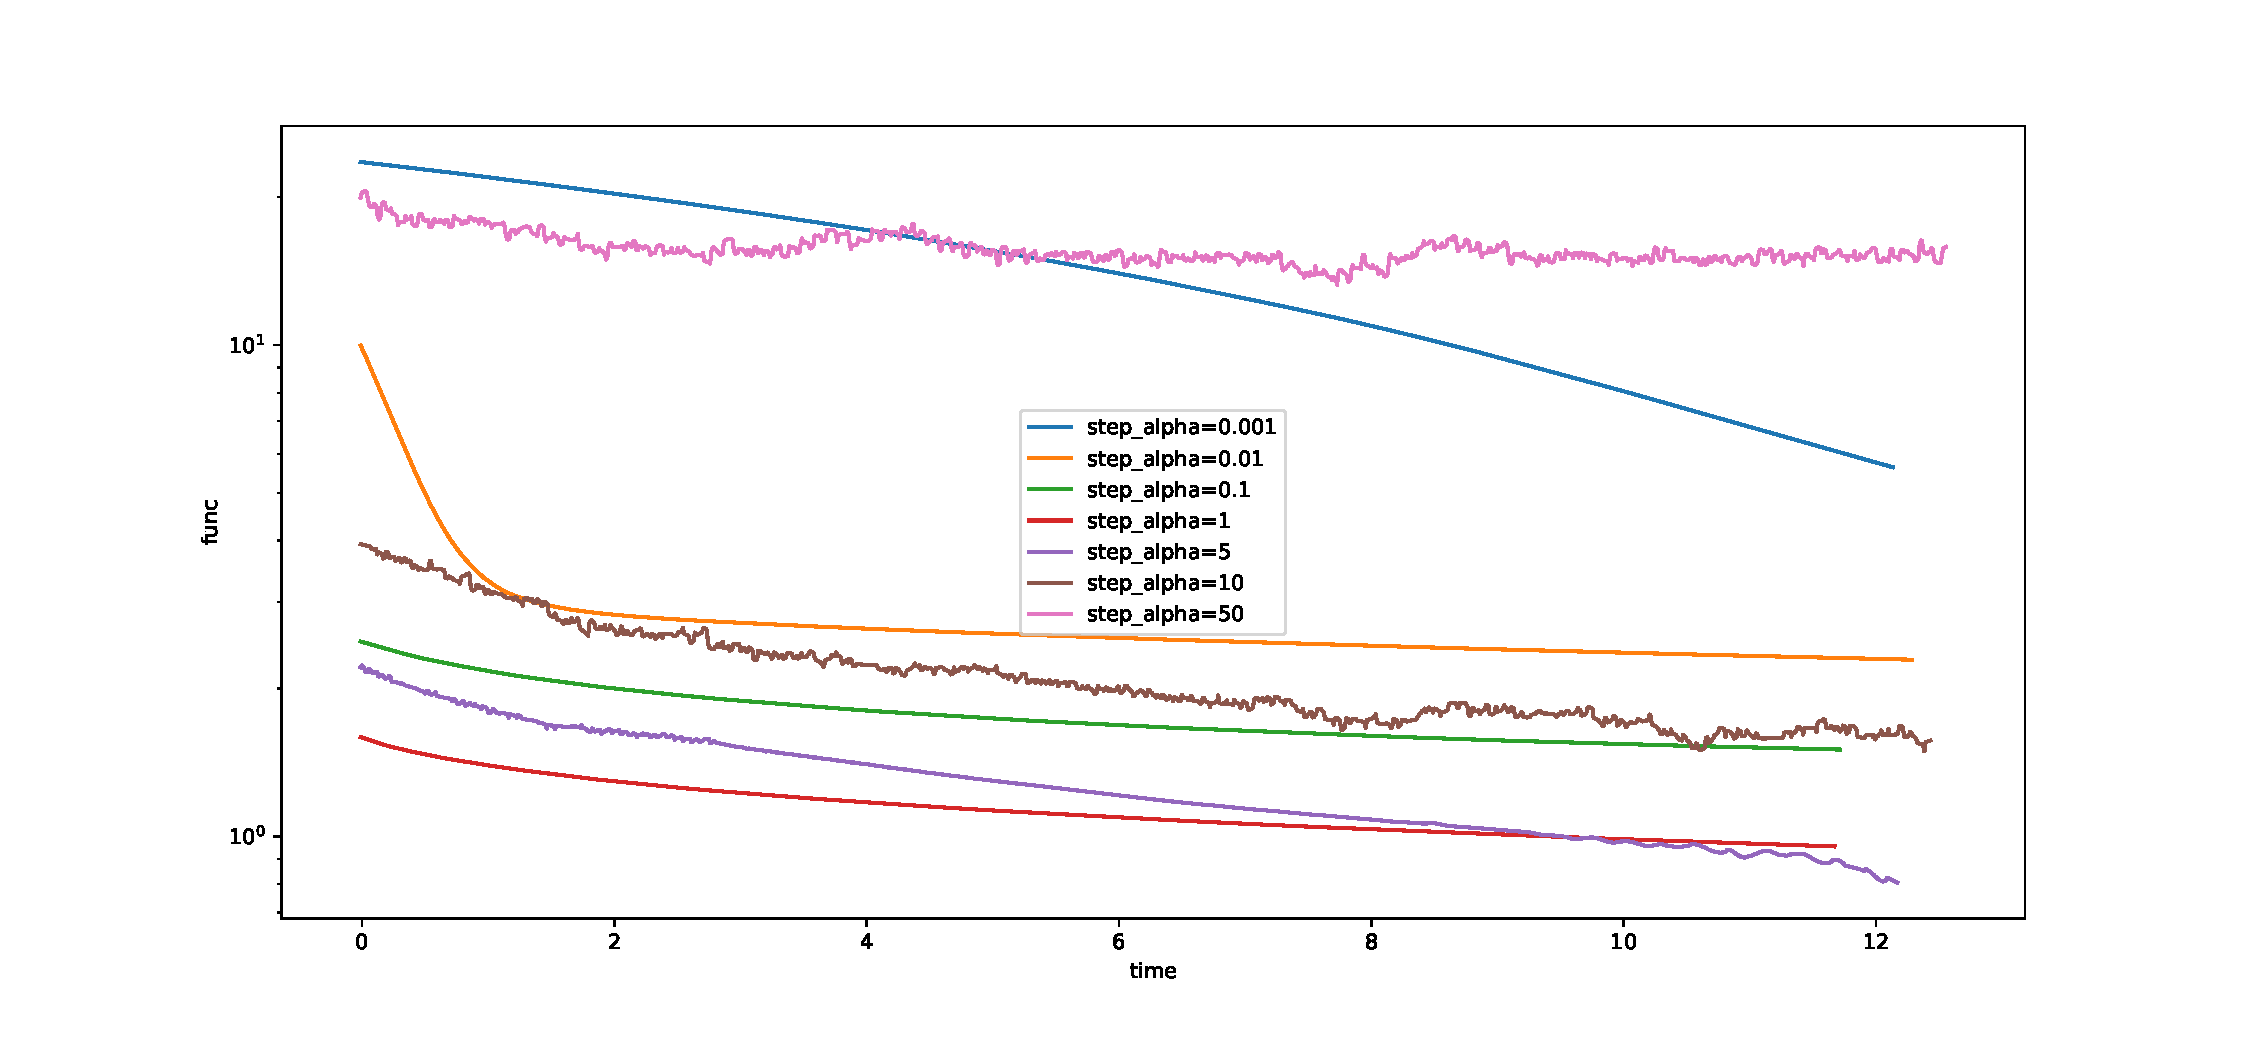
\includegraphics[width=0.5\textwidth, height=0.25\textheight]{../graphs/exp1_func_GD_alpha_time_beta=0,001.pdf}
                        
                        \caption{Зависимость значения точности (accuracy) от эпохи метода градиентного спуска} \label{exp4:sgd_acc_iter}
                        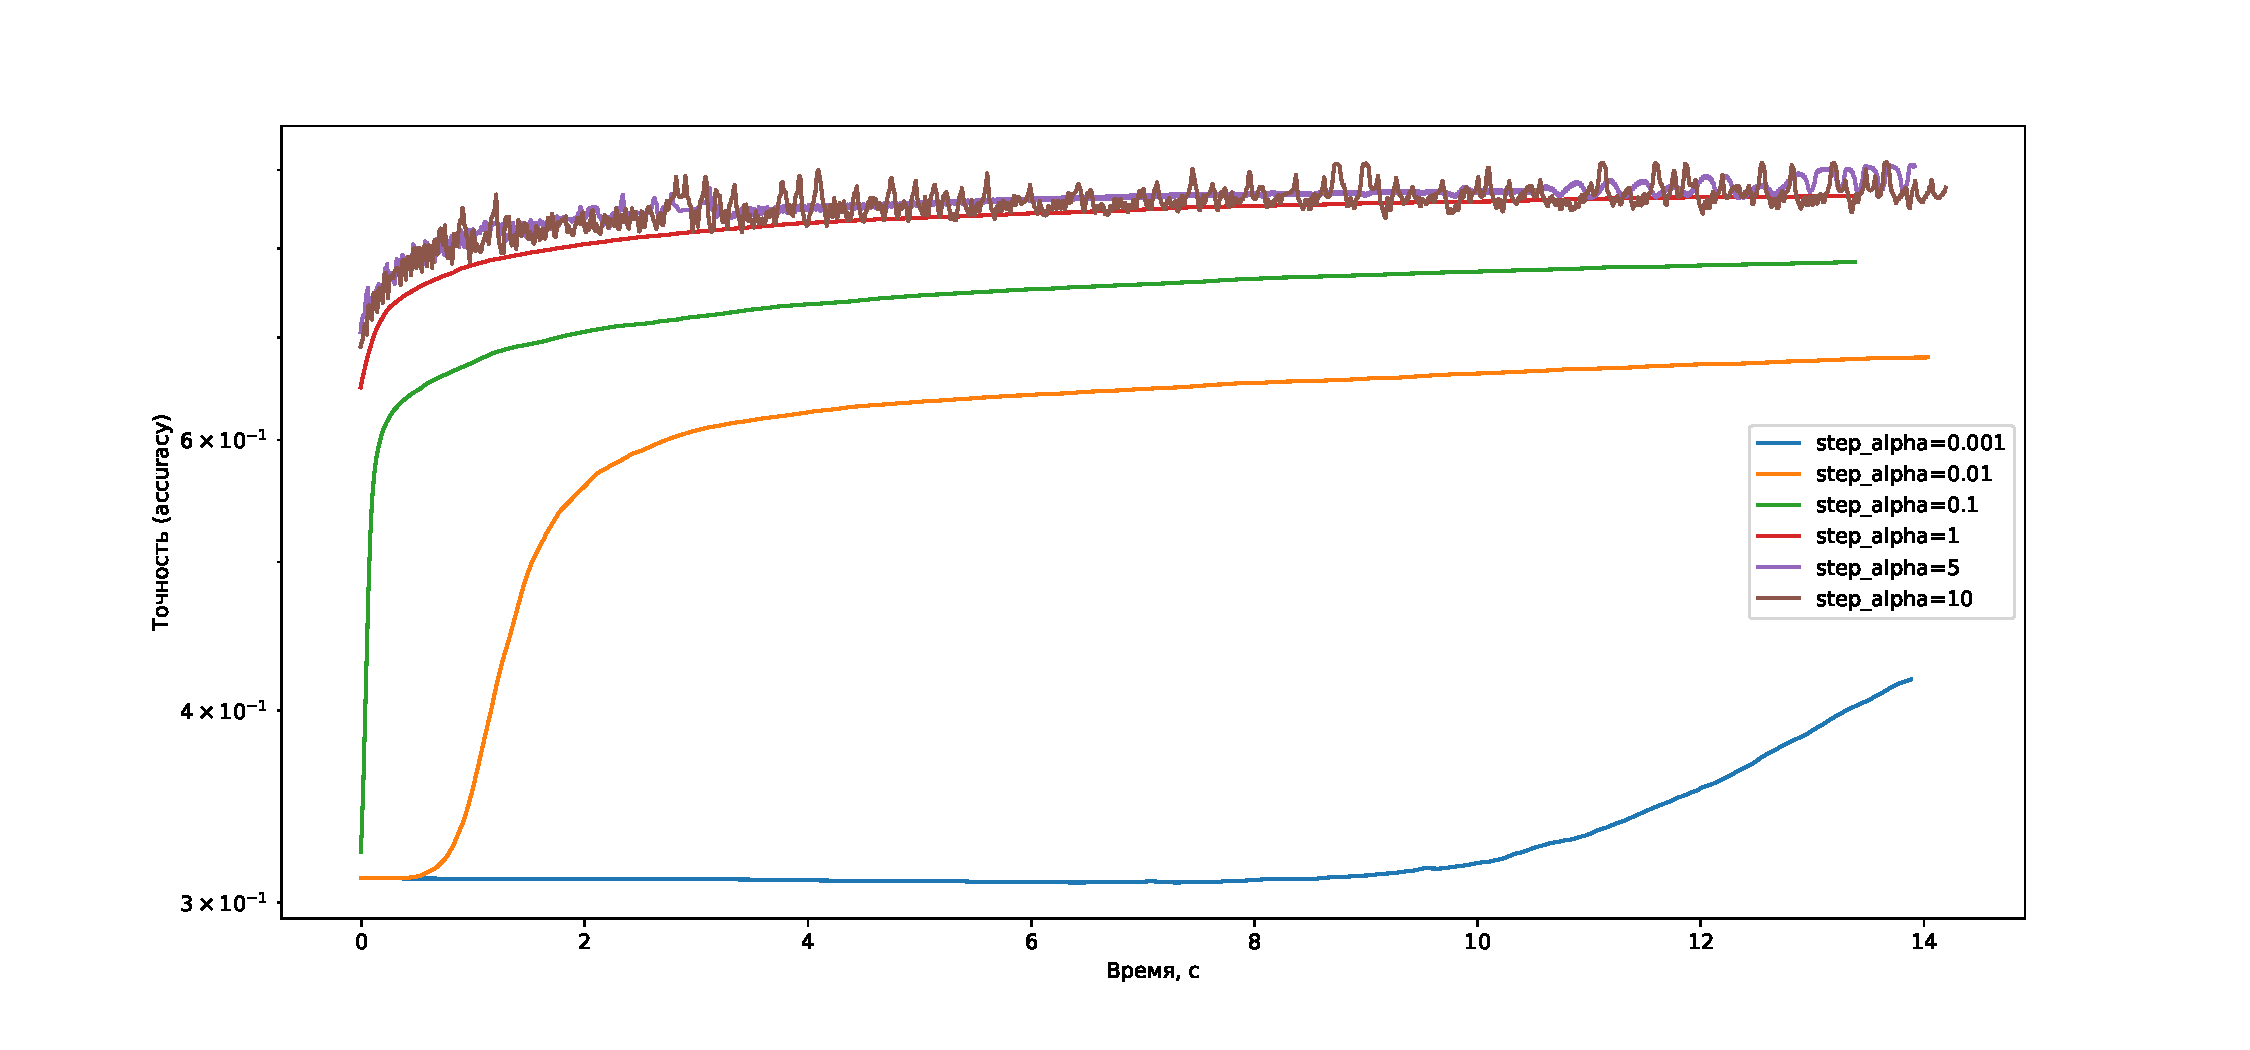
\includegraphics[width=0.5\textwidth, height=0.25\textheight]{../graphs/exp1_accuracy_GD_alpha_time_beta=0,001.pdf}
                    \end{center}
                \end{multicols}
            \end{figure}
            
        \subsection{Сравнение градиентного спуска и стохастического градиентного спуска}
            В данном разделе проведено сравнение методов по трем характеристикам:
            \begin{itemize}
                \item время сходимости метода
                \item точность (accuracy)
                \item значения функции потерь
            \end{itemize}
           Результаты экспериментов приведены на рис. 
            
        \subsection{Лемматизация и удаление стоп-слов}
        
        \subsection{Сравнение представлений BagOfWords и TF-IDF с различными параметрами}
        
    \section{Применение лучших алгоритмов с каждого эксперимента к тестовой выборке}
    
       
        
        
            
\end{document}